\documentclass[12pt,a4paper,twoside,openright]{report}
    \usepackage{amsmath}
    \usepackage{nccmath}
    \usepackage{amsfonts}
    \usepackage{lscape}
    \usepackage[utf8]{inputenc}
    \usepackage{titlepic}
    \usepackage{url} 
    \usepackage{stackengine}
    \usepackage{lipsum}
    \usepackage{enumitem}
    \usepackage[round]{natbib}
    \usepackage{emptypage}
    \usepackage[toc,title,page]{appendix}
    \linespread{1.18} 
    \usepackage[]{graphicx}
    \usepackage[section]{placeins}
    \usepackage{booktabs}
    \usepackage{cite}
	\usepackage{float}
	\usepackage{caption}
	\usepackage{adjustbox}
    \usepackage{subcaption}
    \usepackage{multirow}
    \usepackage[a4paper,width=150mm,top=25mm,bottom=25mm,bindingoffset=-1mm]{geometry}
    \usepackage{fancyhdr}
	\pagestyle{fancy}
	\fancyhead[LE,LO]{Chapter \thechapter}    
     
    \renewcommand{\headrulewidth}{0.05pt}
 
    \usepackage{longtable}
    \usepackage{relsize}
    \usepackage{titlesec}

    \titleformat*{\section}{\large\bfseries}
	\titleformat*{\subsection}{\large\bfseries}
	\titleformat*{\subsubsection}{\small\bfseries}

	\usepackage[T1]{fontenc}
	\usepackage{xcolor}
	\usepackage{lmodern}
	\usepackage{listings}
	\usepackage[]{tocbibind}
    \usepackage{hyperref}
	\let\tmp\oddsidemargin
	\let\oddsidemargin\evensidemargin
	\let\evensidemargin\tmp
	\reversemarginpar



    \usepackage{tikz}
    \usetikzlibrary{shapes.geometric,arrows}
	\makeatletter
    \setlength{\@fptop}{0pt}
    \makeatother
    \tikzstyle{startstop} = [rectangle, rounded corners, minimum width = 4cm, minimum height=1cm, text centered,text width = 5cm, draw = black, fill=white!10]    
     \tikzstyle{process} = [rectangle,  minimum width = 5cm, minimum height=1.5cm, text centered, text width = 5cm,draw = black, fill = white!10]  
	 \tikzstyle{decision} = [diamond, minimum width = 4cm, minimum height=1cm, text centered,text width = 3cm, draw = black, fill = white!10]  
     \tikzstyle{arrow} = [thick,->,>=stealth]  




\newcounter{savepage}
\begin{document}
\begin{titlepage}
	
	\begin{center}
	  	
	  	\vspace*{0.4cm}
	  	
	  	\Large{ \textbf{Development and implementation of user material subroutines for fibre reinforced plastics in a commercial FEM software} }
	  	
	  	\vspace{0.5cm}
	  	
	  	\Large{ \textbf{Master thesis}}
	  	
	  	\vspace{1cm}
	  	
	 \begin{center} \hspace*{0.8cm}	
\includegraphics[width=38mm]{logo.png} \hspace*{0.8cm} \vspace{1cm} \centering 
\includegraphics[width=65mm]{lbf.png} \end{center}
	
	   \vspace{0.5cm}
	   
	 \large { Presented by: Arun Prakash Ganapathy }\\
	  \large { Matriculation number: 63876 } \\
	  \large{Course: Computational Materials Science } \\
	    \large{Institute of Mechanics and Fluid Dynamics}\\
	    	\vspace{1.5cm}
	    	
   \begin{tabular}{l l}

	\vspace{0.2cm}
    \hspace*{1cm} \large{First Examiner:} & \hspace*{1cm}\large{Prof. Dipl.-Ing. Björn Kiefer, Ph.D.}\\
    \vspace{0.2cm}
    \hspace*{1cm} \large{Second Examiner:} & \hspace*{1cm}\large{Dr.-Ing. Stephan Roth}\\
	\vspace{0.2cm}
    \hspace*{1cm} \large{Betreuer:} & \hspace*{1cm}\large{Dr.-Ing. Andreas Seupel} \\

    \hspace*{1cm} \large {External supervisor:} & \hspace*{1cm}\large{Dr.-Ing. Dominik Laveuve }\\
    \hspace*{1cm}  & \hspace*{1cm}\large{Fraunhofer-Institut für Betriebsfestigkeit}\\ 
    \hspace*{1cm}  & \hspace*{1cm}\large{und Systemzuverlässigkeit (LBF) }\\\\  
   \end{tabular}
   
   \vspace*{0.7cm}
    \large { TU Bergakademie Freiberg } \\
     \vspace*{0.3cm}
    \large { August 2021 }
   
   
   
	\end{center}
\end{titlepage}

\clearpage
\thispagestyle{empty}
\hfill
\clearpage
\pagenumbering{Roman}
\vspace*{2cm}
\section*{\LARGE{Abstract} }
\pagestyle{empty}
\indent\indent\indent Composite materials, especially fibre-reinforced plastics, are replacing conventional materials like metals because of their superior strength and lightweight properties not only in advanced structural components but also in everyday applications. Fraunhofer LBF specializes in the safety and reliability of sustainable, lightweight structures. So numerical and experimental analysis and efficient manufacturing of fibre-reinforced plastics are essential in designing and developing lightweight, sustainable, and reliable components. The ongoing project at Fraunhofer LBF investigates the fatigue and creep behaviour of short fibre-reinforced thermoplastics. Therefore, the damage behaviour in composite materials must be understood in order to analyze complex phenomena such as fatigue, creep, etc. The main aim of this master thesis is to develop progressive damage models that can predict the initiation and propagation of damage when the composite material exceeds its failure strength. The constitutive equations necessary for simulating the behaviour of damaged materials are established in the framework of continuum damage mechanics (CDM). Because of the complex material behaviour, anisotropic damage mechanism is employed to represent the damage distribution. Non-linear damage evolution law based on fracture energy regularization technique is utilized to calculate the damage evolution.  First, the damage models are implemented and tested at integration point levels. After that, representative structural examples are used to analyze how the damage models behave under various loading conditions. The global force-displacement response is examined to address the issue related to numerical implementation such as convergence, mesh sensitivity during strain-softening etc. Finally, the damage distribution at the end of the loading process is plotted to visualize the damage propagation in a composite material subjected to loading.



\clearpage
\thispagestyle{empty}
\hfill
\clearpage
\vspace*{2cm}
\section*{\LARGE{Acknowledgement} }
\vspace*{1cm}
\indent\indent\indent   I would like to express my sincere thanks to Dr.-Ing. Dominik Laveuve for his guidance, support and valuable insights throughout this master thesis work.  I would like to extend my gratitude to Prof.Dr.-Ing.Björn Kiefer for providing me the chance to pursue this thesis work under his supervision and Dr.-Ing. Andreas Seupel for his valuable feedback during the thesis work.  I would like to thank Fraunhofer LBF for this opportunity and providing me with the required resources for completion of this thesis work. Last but not least, I am thankful to my friends and family for their constant moral support.



\clearpage
\thispagestyle{empty}
\hfill
\clearpage
\vspace*{2cm}
\section*{\LARGE{Declaration} }
\vspace*{1cm}
\indent\indent\indent Hereby, I  formally declare that I  have developed and written the enclosed thesis 
without illegitimate help of a third party and that no other than the indicated aids have been used for its completion; all thoughts from other sources that have been used literally or indirectly are marked as such. The thesis has not been submitted to any other examination committee in this or a similar form.\\\\\\ Arun Prakash Ganapathy  \\\\\\ .........................................  \\\\ Freiberg, 30.08.2021





\tableofcontents
\listoffigures
\listoftables


\chapter*{List of symbols}
\addcontentsline{toc}{chapter}{\textbf{List of symbols}}

\section*{Symbols for tensors}
\begin{tabular}{l l l}
Scalar  &  Light-face letters  &  a, b,...., A, B,...., $\sigma$, $\epsilon$....,\\
Vectors &  Bold letters        &  \textbf{a}, \textbf{b}...., \textbf{A}, \textbf{B},...., $\mathbf{\Omega}$....,\\
Second-order tensors  &  Underlined letters  &  \underline{a}, \underline{b},...., \underline{A}, \underline{B},....., $\underline{\sigma}$, $\underline{\epsilon}$....,\\  
Fourth-order tensors   &  Uppercase blackboard letters  &   $\mathbb{A}$, $\mathbb{B}$, $\mathbb{C}$.....,\\
\end{tabular}

\section*{Symbols used}
\begin{longtable}{l l}
D &  Damage \\
$\sigma$ & Stress \\
$\tilde{\sigma}$ & Effective stress \\
$\epsilon$ & Strain \\
E  &  Young's modulus \\
$\nu$  &  Poisson's ratio \\
G &  Shear modulus \\
$\mathbf{\Omega}$  &  Damage (vector) \\
$\underline{D}$ &  Damage tensor \\
$\underline{I}$ &  Identity tensor  \\
$\underline{\sigma}$  &  Stress tensor \\
$\underline{\tilde{\sigma}}$  &  Effective stress tensor \\
$\underline{\epsilon}$  &  Strain tensor \\
$\mathbb{M}$  & Damage effect tensor  \\
$\alpha$  &  Internal state variable \\
$\mathbb{S}_{0}$  &  Compliance tensor of an undamaged material \\ 
$\mathbb{S}(D)$  &  Compliance tensor of a damaged material \\ 
$\mathbb{C}_{0}$  &  Elastic stiffness tensor of an undamaged material \\
$\mathbb{C}(D)$  &  Elastic stiffness tensor of a damaged material \\
$F_{I}$ & Failure indices in each principal material direction (I = l, t, z)\\
$X_{t}, Y_{t}, Z{t}$ & Tensile strength in each principal material direction \\ 
$X_{c}, Y_{c}, Z{c}$ & Compressive strength in each principal material direction \\ 
$S$ & Shear strength \\
$\otimes$ & dyadic product \\
$:$ & Double-contraction \\
$.$ & Dot product \\
$\; ^{T}$ & Transpose \\ 
$L_{c}$ & Characteristic element length \\
$G_{f, i}$ & Fracture energy in each principal material direction (i= 1,2,3)\\
$d_{i}$  &  Damage variable in each principal material direction (i= 1,2,3)\\
$P_{i}$  & Softening parameter (i= 1,2,3)\\
\end{longtable}


\chapter*{List of abbreviations}
\addcontentsline{toc}{chapter}{\textbf{List of abbreviations}}
\resizebox{14cm}{5cm}{ 
\begin{tabular}{l l}
 CDM  &  Continuum Damage Mechanics \\

RVE  &  Representative Volume Element \\

FEM  &  Finite Element Methods \\
FE   &  Finite Element \\
IDE  &  Integrated Development Environment \\
USERMAT & User Material routine \\
APDL  &  ANSYS Parametric Design Language \\
TB & Table \\
NTEMPS & Number of Temperature points \\
NPTS & Number of material constants at a given temperature \\
BCs & Boundary Conditions \\
GUI & Graphical User Interface \\
ATS & Alogrithmic Tangent Stiffness \\
CT & Compact Tension\\

\end{tabular}}

\newpage
\setcounter{savepage}{\arabic{page}}
\pagenumbering{arabic}
\pagestyle{fancy}
\fancyhead[RE,RO]{Introduction} 
\chapter{Introduction}
\section{Background and motivation}
\indent\indent\indent Composite materials are made of two or more dissimilar materials of different physical, chemical or mechanical properties, which, when combined, create a material with properties, unlike the individual constituent materials. One of the earliest use of composite materials dates back to 3400 B.C when Mesopotamians glued wood strips at different angles to create plywood \citep{cp}. Nowadays, advanced composite materials are widely used in structural design in various industries such as aerospace, automobile, marine, petrochemical etc., due to their superior properties over traditional engineering materials. \\
\begin{figure}[htbp]
\begin{center}
\includegraphics[width=1\textwidth]{{composite plane.jpg}}
 \caption{Composite materials used in a Boeing 787 'Dreamliner' \citep{cplane} }
 \label{fig:Composite plane}
\end{center}
\end{figure}
\FloatBarrier
\indent\indent\indent Composite materials are attractive because of their high strength, high stiffness-to-density ratio, lightweight properties etc. \citep{lapczyk2007progressive}, Another important reason for using composite materials is the possibility to tailor the stiffness and strength to specific load applications flexibly \citep{wang2009three}. Despite their superior physical properties, composite materials can be damaged from several sources, both during initial processing and in operation. Since composite materials have a complex material response and a low margin of safety through ductility as offered by metals, the development of damage must be understood for predicting failure of such materials \citep{lapczyk2007progressive}. For example, fibre-reinforced plastics exhibit local damage such as fibre breakage, matrix cracking, fibre matrix debonds etc., under normal operating conditions, which may contribute to the failure \citep{maimi2007continuum}. Therefore the ability to predict the initiation and growth of damage is important for predicting the performance, safety and reliability of the composite materials for commercial use.\\

\indent\indent\indent Several methods have been proposed to analyze the failure of composite materials. The simplest of them is to degrade the stiffness of the material instantaneously using a degradation factor once the failure criteria are met \citep{el2015efficient}. While easy to implement, the sudden complete failure of the material does not agree well with the real-life behaviour. Progressive failure analysis of composite materials is required to predict the real-life mechanical behaviour under various loading conditions.  Over the last few decades, the continuum mechanics approach to the damage model based on the works of \citep{kachanov1958rupture} has been employed to analyze the progressive degradation of the materials. The CDM approach provides a methodology that can determine the full range of material deterioration, starting from no damage to the fully disintegrated material. \citep{falzon2011numerical}
\begin{figure}[htbp]
\begin{center}
\includegraphics[width=0.6\textwidth]{{strain-softening.png}}
 \caption{Strain-softening of composite materials after damage initiation \citep{rafi2007analytical}}
 \label{fig:Strain-softening}
\end{center}
\end{figure}
\FloatBarrier
In CDM, the damage is represented as a set of damage variables that describe the material's current state and their development using a set of evolution laws. Once the failure criteria are met, the damage variables are calculated using these evolution laws and the stiffness of the material is degraded with the help of the damage variables \citep{murakami2012continuum} i.e., the material experiences strain-softening rather than strain-hardening observed in metals Figure (\ref{fig:Strain-softening}).  The very fact that the damage can be represented as a set of variables makes them suitable for numerical simulations. Damage formulations can be easily fitted into non-linear finite element (FE) algorithms with the help of constitutive relations and implemented in simulation codes without the need to rely on special discretization technique \citep{peerlings1999enhanced}.

\section{Scope and Outline}
\indent\indent\indent  The objective of the thesis is to develop progressive damage models for predicting the initiation and propagation of the damage in an orthotropic material when subjected to various loading conditions. Continuum damage mechanics (CDM) provides the framework for developing these damage models. Since the composite materials are orthotropic, the model essentially consists of linear elasticity extended with an anisotropic damage mechanism. A second-order orthotropic damage tensor is employed to show the anisotropic damage development. Therefore one damage variable is assigned to each principal material direction to represent the development of damage, i.e., two damage variables are required when the problem is in 2D/Plane-stress and three variables when the problem is in 3D. The numerical modelling of the strain-softening behaviour results in strong mesh dependency, which results in convergence issues when the mesh is refined \citep{wang2009three}. The fracture energy approach is used to reduce the mesh sensitivity, which includes fracture energy in the damage evolution laws. This ensures the objectivity of the model by adjusting the energy dissipated by each failure mechanism using a characteristic element length ($L_{c}$) \citep{falzon2011numerical}.\\
The stages of the thesis work are briefly described as follows\\\\
\textbf{Chapter 2} introduces the theoretical framework of continuum damage mechanics (CDM), constitutive relations and constitutive equations necessary for developing the orthotropic material model. \\\\
\textbf{Chapter 3} gives the reader a brief introduction to software used and the instructions to develop, compile and implement a material model in an FE environment. \\\\
\textbf{Chapter 4} gives a brief introduction to the damage mechanisms, different types of failure criteria and evolution equations necessary for developing damage models. Finally, the chapter deals with the regularization technique used to reduce mesh sensitivity and a brief description of how to implement the damage models numerically. \\\\
\textbf{Chapter 5} The results of the finite element simulations are discussed in this chapter. Starting with the implementation of linear elastic behaviour of the orthotropic material, the chapter discusses the behaviour of the damage models at the integration point level and then using representative structural examples. The issues related to numerical implementation, such as convergence, mesh sensitivity
during strain-softening etc., are also discussed in this chapter



\newpage
\fancyhead[RE,RO]{Continuum damage mechanics} 
\chapter{Continuum damage mechanics}
\indent\indent\indent Continuum damage mechanics (CDM) is a theory for analyzing fracture  and  damage processes in materials from a continuum mechanics point of view. (CDM) provides a continuum perspective for microcracks initiation, propagation, and their coalescence that results in macroscopic damage. CDM uses state variables to represent the damage effect on the stiffness and remaining life of the material that is deteriorating as a result of load and ageing. A failure criteria is required to predict the initiation of damage and evolution laws are required to represent the propagation of damage in material subjected to load \citep{murakami2012continuum}.

\section{Damage}
\indent\indent\indent  Consider a body B of where a crack of length $a$ has developed when subjected to an external load F as shown in Figure. \ref{fig:Damage} . A number of microcracks would be observed around the region arbitrary point P($x$) near the crack tip.
These microcracks are usually developed due to breakage of atomic bonds, or defects in the atomic array \citep{murakami2012continuum}. From the microscopic point of view, fracture of materials is a process of nucleation of microcracks due to the breakage of atomic bonds. From the macroscopic point of view, it is a process of extension of cracks brought about by the coalescence of these microcracks.\\
\indent\indent\indent From the mesoscopic point of view, which exists between microscopic and macroscopic scale, it is a process of nucleation, growth and the coalescence of microscopic cavities that leads to the initiation of macroscopic crack. The development of microscopic, mesoscopic and macroscopic processes of fracture in materials and the resulting deterioration in their mechanical properties is called damage. Continuum damage mechanics aims to analyse the damage development during mesoscopic and macroscopic fracture processes in the framework of continuum mechanics \citep{murakami2012continuum}.
\begin{figure}[htbp]
\begin{center}
\includegraphics[width=0.5\textwidth]{{1. Damage.png}}
 \caption{Scales of damage observation \citep{murakami2012continuum} }
 \label{fig:Damage}
\end{center}
\end{figure}
\FloatBarrier

\section{Representative Volume Element(RVE)}
\indent\indent\indent  To discuss the effects of microcracks in a material using CDM one must homogenize the mechanical effects of microstructure and represent them as a macroscopic continuous field in the material. For this purpose, we take a small region of a mesoscale around the material point P($x$) in body B, as shown in Figure. (\ref{fig:Damage}). We assume that the material with discontinuities in this region as homogeneous, and the state of the material in this region can be represented by the statistical average of the mechanical variables in that region. This region is said to be the Representative Volume Element (RVE) \citep{hill1963elastic} and \citep{hashin1983analysis}. For such RVE, the following two conditions must be satisfied \citep{murakami2012continuum}:
\begin{itemize}
\item  For the material in the RVE to be homogeneous, the RVE should be sufficiently large enough to contain a number of discontinuities
\item To represent a non-uniform macroscopic field by means of a continuum, the size of RVE should be small enough so that the variation of the macroscopic variable in it may be insignificantly small 
\end{itemize}
The size of RVE depends on the microstructure of the relevant material and their typical sizes are as follows \citep{lemaitre2012course}
\begin{itemize}
\item Metals and ceramics  \;    -    \; 0.1\;$mm^3$
\item Polymers and composites \;   -   \; 1\;$mm^3$
\item Timber\; - \; 10\;$mm^3$
\item Concrete \; - \; 100\;$mm^3$
\end{itemize}

\section{Concept of continuum damage mechanics (CDM)}
\indent\indent\indent The basic concept of CDM is that a set of damage variables can represent the microstructural defects in a material. Continuum damage mechanics first represent the state of damage in a material using a set of internal state variables and then describe the mechanical behaviour of the damaged material and then development of damage by use of these state variables. The mechanical behaviour of a damaged material can be described using the notion of effective stress, together with the hypothesis of mechanical equivalence between damaged and undamaged material \citep{murakami2012continuum}. The concept of effective stress and mechanical equivalence will be discussed in the following sections.
\subsection{Modelling by Effective area reduction}
Let us consider body B of Fig. (\ref{fig:Damage2}) and take an RVE at a point $P(x)$ in B. If the total void area in $dA$ is  $ dA_{D} $, the mechanical effect of $dA$ will be decreased by $dA_{D}$. Then the area,
\begin{equation}
  d\tilde{A} = dA  - dA_{D}
  \label{eqn:da} 
\end{equation}
may be interpreted as the area which carries the internal force and is called an $effective$ $area$ \citep{kachanov1986introduction}. Thus, the damage variable D can be specified as 
\begin{equation}
 \label{eqn:D}
  D = \frac{dA - d\tilde{A}}{dA} = \frac{dA_{D}}{dA}
\end{equation}
where the damage variable D takes a value between 0 and 1 ($0 \leq D \leq 1$). $D = 0$ represents initial undamaged state and $D=1$ represents fully damaged state.
\begin{figure}[htbp]
\begin{center}
\includegraphics[width=0.8\textwidth]{{Damage2.png}}
 \caption{Effective area reduction due to microcracks \citep{murakami2012continuum}}
 \label{fig:Damage2}
 \end{center}
\end{figure}
\FloatBarrier
Suppose a cylindrical bar of cross-sectional area $dA$ is subject to a tensile load $dF$, then the actual load carrying area is $ d\tilde{A}$ rather than $dA$. According to eqns (\ref{eqn:da}) and (\ref{eqn:D}) the effective area $ d\tilde{A}$ is given by,
\begin{equation}
\label{eqn:da_t}
 d\tilde{A} = (1-D)dA
\end{equation}
The decrease in the load-carrying area increases the effect of stress $\sigma$ induced by the external force $dF$. Due to eqn \ref{eqn:da_t}, the magnified stress $\tilde{\sigma}$ is given by,
\begin{equation}
\label{eqn:sig_t}
\tilde{\sigma} = \frac{dF}{d\tilde{A}} = \frac{\sigma}{1 - D}
\end{equation} 

Since the stress $\tilde{\sigma}$ represents the stress magnified by the net area reduction due to damage, it is called  $effective$ $stress$    \citep{kachanov1986introduction}. From eqn (\ref{eqn:da_t}) and (\ref{eqn:sig_t}) we can postulate that the damaged cylindrical bar of Figure.(\ref{fig:Damage3}b) with the cross-sectional area $dA$ subject to force $dF$ is mechanically equivalent to the  fictitious  undamaged bar of Figure.(\ref{fig:Damage3}c), which is subject to force $dF$, has the cross-sectional area $ {d\tilde{A}} $ and hence stress $\tilde{\sigma}$ . (Note - The concept and equations in this section are derived from \citep{murakami2012continuum})
\begin{figure}[htbp]
\begin{center}
\includegraphics[width=0.8\textwidth]{{3. Damage_cylinder.png}}
 \caption{Damage of bar under tensile load \citep{murakami2012continuum}}
 \label{fig:Damage3}
 \end{center}
\end{figure}
\FloatBarrier

\subsection{Modelling by variation of elastic modulus} 
\indent\indent\indent Since the development of microcracks causes the reduction in material stiffness, the damage state can be characterized by variation in elastic modulus \citep{lemaitre1978aspect}. Let us consider the bar (b) and (c) of Figure. (\ref{fig:Damage3}) are in the damaged and fictitious undamaged state, respectively. Then the elastic strain $\epsilon$ in the bar (c) due to stress $\tilde{\sigma}$ should be equal to the $\epsilon$ of the bar (b) under stress $\sigma$; i.e.,\\
\begin{equation}
\label{eqn:sig_t2}
   \tilde{\sigma} = E_{0}\epsilon, \;\;  \sigma = E(D)\epsilon 
\end{equation}
\\
\begin{equation}
\label{eqn:epsilon}
\epsilon = \frac{\sigma}{E(D)} = \frac{\tilde{\sigma}}{E_{0}}
\end{equation}
where $E_{0}$ and $E(D)$ are the young's modulus of the material in the initial undamaged state and in damaged state after loading, respectively. Therefore, eqn. (\ref{eqn:epsilon}) defines another effective stress\\
\begin{equation}
\label{eqn:epsilon2}
  \tilde{\sigma} = \frac{E_{0}}{E(D)}\sigma
\end{equation}
By combining Eqn. (\ref{eqn:sig_t}) and (\ref{eqn:epsilon}) we get,
\begin{equation}
\label{eqn:E(d)}
E(D) = (1 - D) E_{0}
\end{equation}
\begin{equation}
\label{eqn:D2}
D  = 1 - \frac{E(D)}{E_{0}}
\end{equation}
Therefore, the damage variable $D$ is characterized by the variation in Young's modulus $E(D)$. The modelling of damage by means of reduction in stiffness can be applied also to the anisotropic damage of brittle materials like composite materials, concrete, rocks etc., (Note - The concept and equations in this section are derived from \citep{murakami2012continuum})


\section{Mechanical representation of the damage state}
\indent\indent\indent The deformation of material depends on the direction of applied stress or strain, and hence it is an anisotropic phenomena. Therefore different theories have been developed for modelling 3-D anisotropic damage phenomenon \citep{murakami2012continuum}. Some fundamental theories that describe 3-D damage state are given below. 
\subsection{Scalar damage variable}
\indent\indent\indent In the case of random or isotropic distribution of microcracks or voids, and when void density is small, the global mechanical properties can be approximated as nearly isotropic. The damage state, in this case, may be represented using scalar damage variable D. Thus isotropic damage theory based on isotropic damage variable can be applied to 3-D problems of creep, elastic-plastic, ductile and fatigue damage \citep{lemaitre2012course}
\subsection{Vector damage variable}
\indent\indent\indent The damage state can be specified by the decrease in load carrying effective area due to void development. Hence it is easy to postulate a vector damage variable.  \citep{kachanov1986introduction} tried to extend the definition of damage to anisotropic damage by noting a surface element in an arbitrary direction $n$, he proposed vector damage variable $ \mathbf{\Omega} = \Omega_{n} \mathbf{n} $, where $\Omega_{n}$ is the effective area fraction. 
\subsection{Damage tensor of second order}
\indent\indent\indent To describe an anisotropic damage state, a damage variable of second or higher order tensor is required. Eqn.(\ref{eqn:da_t}) suggests that the damage state (1 - D) is specified by the transformation of the surface element $dA$ of Fig. (\ref{fig:Damage3}b) of the damage state into the corresponding surface element $d\tilde{A}$ in the fictitious undamaged state of Fig.(\ref{fig:Damage3}c) \citep{murakami2012continuum}. 
\begin{figure}[htbp]
\begin{center}
\includegraphics[width=0.7\textwidth]{{4. Damage.png}}
 \caption{Surface element in RVE of a damaged material \citep{murakami2012continuum}}
 \label{fig:Damage4}
 \end{center}
\end{figure}
\FloatBarrier
To express damage as a second order tensor, we first consider an arbitrary surface element $PQR$ in RVE in the current damaged configuration $B_{t}$ of Fig.(\ref{fig:Damage4}a). The unit normal vector and area of $PQR$ are denoted by $\nu$ and $dA$. We further postulate the fictitious undamaged configuration $B_{f}$ of Fig.(\ref{fig:Damage4}b) mechanically equivalent to $B_{t}$, and the surface element and its area vector are denoted by $\tilde{P}\tilde{Q}\tilde{R}$ and $\tilde{\nu}d\tilde{A}$ respectively. According to Eqn.(\ref{eqn:da_t}) the damage variable of second-order tensor $D$ should be defined by linear transformation from area vector $\nu dA$ in $B_{t}$ into $\tilde{\nu}d\tilde{A}$ in $B_{f}$, i.e.,
\begin{equation}
\label{eqn:second_order_tensor}
\underline{\tilde{\nu}} d\tilde{A} = (\underline{I} - \underline{D})\underline{\nu} dA
\end{equation}
where $I$ is the second order identity tensor. Since the damage tensor $D$ is symmetric, it can be expressed by its spectral decomposition
\begin{equation}
\label{eqn:damage_2nd_order}
\underline{D} = \sum_{i = 1}^{3} D_{i}\mathbf{n_{i}}  \otimes D_{i}\mathbf{n_{i}}
\end{equation}
where $D_{i}$ and $n_{i}$ are the principal values and principal directions of $D$. (Note - The concept and equations in this section are derived from \citep{murakami2012continuum})

\section{Effective Stress Tensors}
\indent\indent\indent The effective stresses are used to describe the mechanical behaviour of the damaged material. Some of the effective stresses postulated in damage mechanics are given below
\subsection{Effective stress tensor for isotropic damage \citep{lemaitre1978aspect}}
\indent\indent\indent If the damage state is isotropic then the effective stress tensor of three-dimensional state is given by
\begin{equation}
 \underline{\tilde{\sigma}} = (1 - D)^{-1} \; \underline{\sigma}
\end{equation}
where D is the scalar damage variable, and $\sigma$ is the Cauchy stress tensor. This effective stress simplifies damage theory and can be applied to a number of damage problems like ductile damage. But this cannot be applied to damage of significant anisotropy, such as brittle damage due to microcrack distribution.\\
\subsection{Asymmetric effective stress tensor for anisotropic damage \citep{murakami2012continuum}}
\indent\indent\indent The increase in stress caused by the net area reduction in case of anisotropic damage is given by
\begin{equation}
\underline{\tilde{\sigma}} = (\underline{I} - \underline{D})^{-1} \; \underline{\sigma}
\label{eqn:assymetric}
\end{equation}
where I and D are second-order identity tensor and the second-order damage tensor, respectively. In the actual development of anisotropic damage, the stress-induced in the RVE of damage material is asymmetric. But asymmetric stress tensors make the numerical analysis complicated, and thus different methods of symmetrization have been proposed. A few of them are described as follows

\subsection{Symmetrized effective stress tensor for anisotropic damage \citep{murakami2012continuum}} 
\indent\indent\indent A simple symmetrization procedure of Eq.(\ref{eqn:assymetric}) gives,
\begin{equation}
\label{eqn: Murakami and Ohno}
\underline{\tilde{\sigma}} = \frac{1}{2} [(\underline{I} - \underline{D})^{-1}\;\underline{\sigma} + \underline{\sigma}(\underline{I} - \underline{D})^{-1}]
\end{equation}

\section{Damage effect tensors}\label{Matrix Representation of Damage effect tensors}
\indent\indent\indent The general form of an effective stress tensor $\underline{\tilde{\sigma}}$ is given by the damage effect tensor $\mathbb{M}$ and the corresponding Cauchy stress tensor $\underline{\sigma}$, i.e.,
\begin{equation}
\underline{\tilde{\sigma}}  = \mathbb{M} \; :  \underline{\sigma}
\label{eqn:effective_stress_tensor} 
\end{equation}
It is convenient to express the tensors in the form of matrices and then execute the tensor operations as a matrix calculus.. To simplify this procedure, we take an orthonormal basis ${n_{i}}$ with principal directions $n_{i}$ of the second-order symmetric damage tensor $D$, and represent the tensor in terms of its component to this basis \citep{murakami2012continuum}. According to Voigt notation, the second-order symmetric tensor $\underline{\sigma}$ and the related effective stress $\underline{\tilde{\sigma}}$ are expressed by the column vector of six dimensions:
\begin{equation}
   [\sigma_{P}]  \equiv  [\sigma_{11} \;\; \sigma_{22} \;\;\sigma_{33} \;\;\sigma_{12} \;\;\sigma_{13} \;\;\sigma_{23} ]^{T}
\end{equation}

\begin{equation}
   [\tilde{\sigma_{P}}]  \equiv  [\tilde{\sigma_{11}} \;\; \tilde{\sigma_{22}} \;\;\tilde{\sigma_{33}} \;\;\tilde{\sigma_{12}} \;\;\tilde{\sigma_{13}} \;\;\tilde{\sigma_{23}} ]^{T}
\end{equation}
\\
By means of the matrix representation, we have the matrix form
\begin{equation}
[\tilde{\sigma_{P}}] \equiv [\mathbb{M}_{pq}]\;: [\sigma_{P}]
\label{eqn:Matrix_rep_damage_effect_tensor}
\end{equation}
\\
Matrix representation of the damage effect tensor of Eq.(\ref{eqn:Matrix_rep_damage_effect_tensor}) is shown below \citep{wang2009three}
\\
$$
\mathlarger{ [\mathbb{M}_{pq}] \equiv   
 \begin{bmatrix}
   \; \frac{1}{\omega_{11}}  \; & 0 \; & 0 \; & 0 \; & 0\; & 0  \;\\
  \\
   \;0\; & \frac{1}{\omega_{22}}\; & 0\; & 0\; & 0\; & 0  \;\\
  \\
  \; 0\; & 0 \; & \frac{1}{\omega_{33}}\; & 0\; & 0\; & 0 \; \\
  \\
   \; 0\; & 0\; & 0\; & \frac{1}{\omega_{12}}\; & 0\; & 0  \;\\
  \\
   \; 0\; & 0\; & 0\; & 0\; & \frac{1}{\omega_{23}}\; & 0  \;\\
  \\
   \; 0\; & 0\; & 0\; & 0\; & 0\; & \frac{1}{\omega_{13}}  \; 
  \\
 \end{bmatrix}}
 \label{Damage_effect_tensor}
 $$
\\
where
$$\omega_{11} \; = \; (1 - d_{1}); \;\;  \omega_{22} \; = \; (1 - d_{2}); \;\; \omega_{33} \; = \; (1 - d_{3});$$ \vspace*{0.1cm} $$\omega_{12} \; = \; \sqrt{(1 - d_{1})(1 - d_{2})};  \;\;\omega_{23} \; = \; \sqrt{(1 - d_{2})(1 - d_{3})}; \;\; \omega_{13} \; = \; \sqrt{(1 - d_{1})(1 - d_{3})};$$

\section{Hypothesis of strain Equivalence}\label{Hypothesis of Strain Equivalence}

\indent\indent\indent The constitutive equation of a damaged material is given by the constitutive equation for an undamaged material by replacing the stress tensor $\underline{\sigma}$ in the equation with the effective stress $\tilde{\sigma}$ \citep{lemaitre1978aspect}.  The stress $\underline{\sigma}$ acting on RVE in the damaged configuration $B_{t}$ is equivalent to that of the stress $\underline{\tilde{\sigma}}$ in the fictitious undamaged configuration in Figure (\ref{fig:Strain_eq}).. Therefore the deformation of the damaged material subject to stress $\underline{\sigma}$ should be equal to that of the fictitious undamaged material subject to stress $\underline{\tilde{\sigma}}$. Suppose the constitutive equation of an undamaged material is given by
\begin{equation}
  \epsilon = F_{0}(\underline{\sigma}, \alpha)
\end{equation} 
or
\begin{equation}
  \dot{\epsilon} = F_{0}(\underline{\sigma}, \alpha)
\end{equation}

where $\alpha$ is an internal variable representing the internal change other than damage. and ($\dot{}$) denotes the material time derivative.
\begin{figure}[htbp]
\begin{center}
\includegraphics[width=0.8\textwidth]{{6. Strain_eq.png}}
 \caption{Hypothesis of strain equivalence \citep{murakami2012continuum}}
 \label{fig:Strain_eq}
 \end{center}
\end{figure}
Then according to hypothesis of strain equivalence, the inelastic constitutive equation of the damaged material represented by a damage variable $D$ should be given by replacing $\underline{\sigma}$ of Eq.(25) with the effective stress $\underline{\tilde{\sigma}}$ i.e.,

\begin{equation}
    	\underline{\epsilon} = F(\underline{\sigma}, D, \alpha)  = F_{0}(\underline{\tilde{\sigma}}, \alpha)
\end{equation}

or 
\begin{equation}
    	\dot{\underline{\epsilon}} = F(\underline{\sigma}, D, \alpha)  = F_{0}(\underline{\tilde{\sigma}}, \alpha)
\end{equation}

In case of elastic deformation, constitutive equations for an undamaged and damaged material are given by
\begin{equation}
\underline{\epsilon} = \mathbb{S}_{0}\; : \underline{\sigma},
\end{equation}\\
\begin{equation}
\underline{\epsilon} = \mathbb{S}(D)\; : \underline{\sigma},
\end{equation}
where $\mathbb{S}_{0}$ and $\mathbb{S}(D)$  are fourth-order elastic compliance tensors of the materials. Therefore, according to the hypothesis of strain equivalence the elastic constitutive equation of the damaged material and the compliance tensor are given by 
\begin{equation}
\underline{\epsilon} = \mathbb{S}_{0}\; : \underline{\tilde{\sigma}}  =  [\mathbb{S}_{0}\;: \mathbb{M} (D)]\;: \underline{\sigma} = \mathbb{S}(D)\; : \underline{\sigma}
\end{equation}
\begin{equation}
\mathbb{S}(D) = \mathbb{S}_{0}\; : \mathbb{M} (D)
 \label{eqn:S_HSeq}
\end{equation}
where $\mathbb{M} (D)$ is the damage effect tensor which is given by 
\begin{equation}
\mathbb{M} (D)  = \mathbb{S}_{0}^{-1} \; : \mathbb{S}(D) 
\end{equation}
(Note - The concept and equations in this section are derived from \citep{murakami2012continuum})

\section{Hypothesis of strain energy equivalence}\label{Hypothesis of strain energy equivalence}
\indent\indent\indent The existence of a strain energy function necessitates the symmetry of the compliance and elastic modulus tensor. But the compliance tensor resulting from the hypothesis of strain equivalence is asymmetric which does not satisfy the requirement. Therefore the hypothesis of strain energy equivalence is used to satisfy the symmetry requirements \citep{cordebois1982damage}. Let us consider an elastic-plastic material and represent the plastic deformation by an internal state variable $\alpha$. The complementary strain energy functions of the material at undamaged and damaged state are given, respectively as follows
\\
\begin{equation}
V_{0}(\underline{\sigma},\alpha) = \frac{1}{2}\underline{\sigma} : \mathbb{S}_{0} : \underline{\sigma} \; - \; \phi(\alpha)
\end{equation}
\\
\begin{equation}
V(\underline{\sigma},D,\alpha) = \frac{1}{2}\underline{\sigma}: \mathbb{S}(D) : \underline{\sigma} \; - \; \phi(\alpha)
\end{equation}
\\
Thus the constitutive equation for the undamaged and damaged material is 
\\
\begin{equation}
\epsilon = \frac{\partial V_{0} }{\partial \underline{\sigma}} = \mathbb{S}_{0} : \underline{\sigma}
\end{equation}
\\
\begin{equation}
\epsilon = \frac{\partial V }{\partial \underline{\sigma}} = \mathbb{S}(D) : \underline{\sigma}
\label{eqn:Strain_energy_eq}
\end{equation}

\begin{figure}[htbp]
\begin{center}
\includegraphics[width=0.8\textwidth]{{7.Strain_energy_eq.png}}
 \caption{Hypothesis of strain energy equivalence \citep{murakami2012continuum}}
 \label{fig:Strain_energy_eq}
 \end{center}
\end{figure}
Suppose a damaged material of Figure.(\ref{fig:Strain_energy_eq})a subject to stress $\underline{\sigma}$, and represent the damage and internal state due to inelastic deformation by $D$ and $\alpha$, respectively. Then the strain energy function $V(\underline{\sigma},D,\alpha)$ of the damaged material is given by replacing $\underline{\sigma}$ in the corresponding function $V_{0}(\underline{\sigma},\alpha)$ of the undamaged material of Fig.(\ref{fig:Strain_energy_eq})b with the effective stress $\tilde{\sigma}$
\\
\begin{equation*}
V(\underline{\sigma},D,\alpha) \; = \; V_{0}(\underline{\tilde{\sigma}},\alpha)
\end{equation*}
\\
By the use of this hypothesis, the elastic strain of Eq.(\ref{eqn:Strain_energy_eq}) leads to
\\
\begin{equation*}
\underline{\epsilon} \; = \; \frac{\partial V(\underline{\sigma},D,\alpha)}{\partial \underline{\sigma}} = \mathbb{S}(D) : \underline{\sigma}
\end{equation*}
\\
\begin{equation*}
\;\;\;\;\;\;\;\;\;\; = \; \frac{\partial V_{0}(\underline{\tilde{\sigma}},\alpha)}{\partial \underline{\sigma}} = \frac{\partial}{\partial \underline{\sigma}}(\frac{1}{2}\underline{\tilde{\sigma}} : \mathbb{S}_{0} : \underline{\tilde{\sigma}} )
\end{equation*}
\\
\begin{equation*}
\;\;\;\;\;\;\;\;\;\;\;\;\;\;\;\;\;\; = \; \frac{1}{2}\frac{\partial}{\partial \underline{\sigma}} [(\mathbb{M}(D):\underline{\sigma}) : \mathbb{S}_{0} : (\mathbb{M}(D):\underline{\sigma})]
\end{equation*}
\\
\begin{equation}
= \;[\mathbb{M}^{T}(D) : \mathbb{S}_{0} : \mathbb{M}(D)]
\label{M_eqn}
\end{equation}
\\
From Eq.(\ref{M_eqn}), the elastic compliance tensor of the damaged material is given as follows
\\
\begin{equation}
\mathbb{S}(D) \; = \; \mathbb{M}^{T}(D) : \mathbb{S}_{0} : \mathbb{M}(D)
\label{eqn: S_HSEeq}
\end{equation}
\indent\indent\indent If the damage effect tensor $\mathbb{M}(D)$ can be expressed as a fourth-order symmetric tensor, then the elastic compliance tensor $\mathbb{S}(D)$ becomes a fourth-order symmetric tensor which satisfies the symmetry requirement. (Note - The concept and equations in this section are derived from \citep{murakami2012continuum}) 

\section{Elastic constitutive equation and elastic modulus tensor of orthotropic material}\label{Constitutive matrix}
\indent\indent\indent Orthotropic materials are materials that exhibit different material properties in the mutually perpendicular directions. They are a special form of anisotropic materials because their properties change when measured from different directions. Some examples of orthotropic materials are wood, composite materials etc., Orthotropic materials require 9 independent variables to express their constitutive matrix \citep{ortho}. The 9 elastic constants are three Young's moduli $E_{x},E_{y},E_{z}$, the three Poisson's ratios $\nu_{xy},\nu_{yz},\nu_{zx}$, and three shear moduli $G_{xy},G_{yz},G_{zx}$. The constitutive equation and elastic stiffness matrix of orthotropic material \citep{lempriere1968poisson} has the form,

\begin{equation}
  \underline{\sigma} = \mathbb{C}_{0} : \underline{\epsilon} \;\;\;   or \;\;\;  \sigma_{ij}  =  C^{0}_{ijkl}\epsilon_{kl},
\end{equation}

$$
\mathlarger{ [C^{0}_{pq}]} =  
 \begin{bmatrix}
 \mathlarger{ \frac{1 - \nu_{yz}\nu_{zy}}{E_{y}E_{z}\Delta} } \;&  \mathlarger{  \frac{\nu_{xy} + \nu_{xz}\nu_{zy}}{E_{y}E_{z}\Delta}}   \;& \mathlarger{  \frac{\nu_{xz} + \nu_{xy}\nu_{yz}}{E_{y}E_{z}\Delta} }  \;&  \mathlarger{  0}  \;&  \mathlarger{ 0}  \;& \mathlarger{  0}  \\
 \\
    \mathlarger{ \frac{\nu_{yx} + \nu_{yz}\nu_{zx}}{E_{x}E_{z}\Delta} }  \;& \mathlarger{  \frac{1 - \nu_{xz}\nu_{zx}}{E_{1}E_{z}\Delta} }\; & \mathlarger{ \frac{\nu_{yz} +\nu_{yx}\nu_{xz}}{E_{1}E_{z}\Delta} } \; & \mathlarger{ 0}\; &\mathlarger{  0}\; & \mathlarger{ 0}\\
  \\
   \mathlarger{  \frac{\nu_{zx} + \nu_{yx}\nu_{zy}}{E_{x}E_{y}\Delta}}  \;& \mathlarger{   \frac{\nu_{zy} + \nu_{xy}\nu_{zx}}{E_{x}E_{y}\Delta} }\;&\mathlarger{  \frac{1 - \nu_{xy}\nu_{yx}}{E_{x}E_{y}\Delta} } \;&\mathlarger{  0 }\;& \mathlarger{ 0 }\;&\mathlarger{  0} \\ 
\\

 
 \mathlarger{  0} \;&  \mathlarger{  0 } \;&  \mathlarger{  0 }\;&\mathlarger{ G_{xy}} \;& \mathlarger{0} \;& \mathlarger{0} \\
  \\
 \mathlarger{ 0} \;&  \mathlarger{  0 }\;&  \mathlarger{  0 } \;& \mathlarger{0 }\;& \mathlarger{ G_{yz} }\;&\mathlarger{ 0} \\
  \\
  \mathlarger{0}\;&  \mathlarger{  0 } \;&  \mathlarger{  0 } \;& \mathlarger{0 }\;& \mathlarger{0} \;& \mathlarger{G_{zx}} 
 \end{bmatrix}
 $$\\
 
 where 
 \begin{align*}
\mathlarger{ \Delta = (1 - \nu_{xy}\nu_{yx} - \nu_{yz}\nu_{zy} - \nu_{zx}\nu_{xz} - 2\nu_{xy}\nu_{yz}\nu_{zx})/E_{x}E_{y}E_{z}}
 \end{align*}
   and  $\mathlarger{\frac{\nu_{xy}}{E_{y}} = \frac{\nu_{yx}}{E_{x}}, \frac{\nu_{yz}}{E_{z}} = \frac{\nu_{zy}}{E_{y}}, \frac{\nu_{xz}}{E_{z}} = \frac{\nu_{zx}}{E_{x}} }$ 


\newpage
\fancyhead[RE,RO]{Working environment} 
\chapter{Working environment}
\vspace*{1cm}
\indent\indent\indent  The material models necessary for simulating damage must be programmed first using a programming language, compiled, and then tested in a commercial FEM software. The programming language of choice for most commercial FEM software is FORTRAN because it is fast and efficient. To program the material model, an integrated development environment (IDE) and a compiler compatible with the version of the FEM software are required. This chapter describes the tools required for creating damage models and instructions on how to use them in order to test the models in detail.   
\vspace*{1cm}
\section{Software tools required}
\begin{itemize}
\item \textbf{GNU Octave}\\ \indent
\hspace*{13mm} GNU Octave is software which uses a high-level programming language primarly intended for numerical computations. Initially, the damage models are developed on Octave and tested using simple loading cases like uniaxial tension with the help of constitutive driver routines before implementing them as user material routine (USERMAT) in ANSYS. 
\item \textbf{Microsoft Visual Studio }\\
\hspace*{13mm} Microsoft Visual Studio is the IDE used for programming the damage models as user material routines using the FORTRAN programming language.
\item \textbf{Intel parallel studio}\\
\hspace*{13mm} The compiler available in Intel parallel studio is used for compiling the USERMAT before testing them in a FEM software.
\item \textbf{ANSYS }\\
\hspace*{13mm}ANSYS is the commercial FEM software chosen for creating models of specimens and analyzing damage models behave under different loading conditions.
\end{itemize}

The following sections provide the reader with a detailed description, starting from developing the user material routine to implementing and analysing the results in the ANSYS environment.  The flowchart below shows the steps involved in the whole process\\
\begin{center}
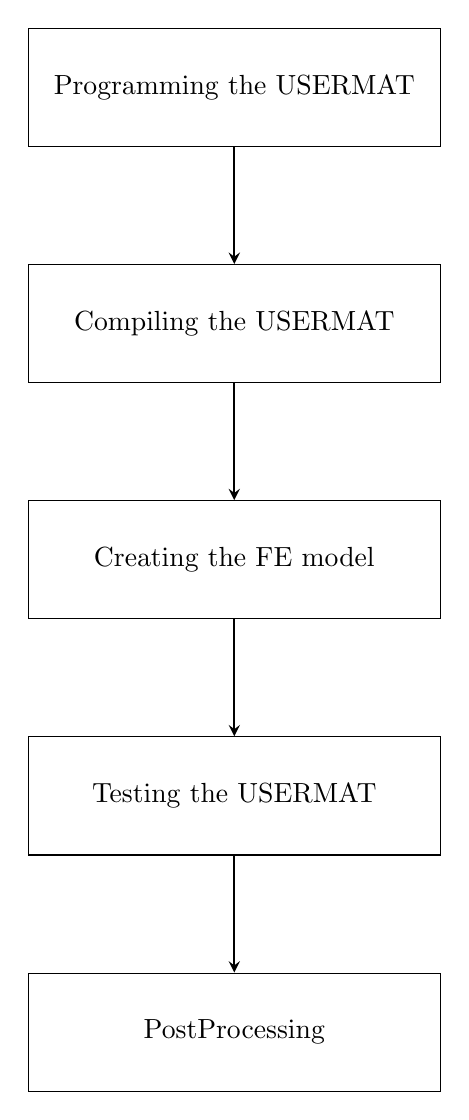
\begin{tikzpicture}[node distance = 3cm]

\node(start) [process] {Programming the USERMAT};
\node(compile) [process, below of = start] {Compiling the USERMAT};
\node(Model)   [process, below of = compile] {Creating the FE model};
\node(solve) [process, below of = Model] {Testing the USERMAT};
\node(post)[process, below of = solve] {PostProcessing};


\draw [arrow] (start) -- (compile);
\draw [arrow] (compile) -- (Model);
\draw [arrow] (Model) -- (solve);
\draw [arrow] (solve) -- (post);


\end{tikzpicture}
\FloatBarrier
\label{Schematic of USERMAT implementation}
\end{center}
\vspace*{0.6cm}
\section{Programming the USERMAT}
\indent\indent\indent  The user material routine (USERMAT) is an ANSYS programmable feature which allows users to write their own material constitutive equations within a newly developed general material framework \citep{lin1999ansys} . The subroutine is called at all material integration points of the element during the solution phase.\\
\indent\indent\indent ANSYS demands the necessary variables declared in a certain way so that the USERMAT developed can work compatibly with ANSYS when it is called at each integration point. The guidelines for declaring input and output arguments can be found on ANSYS' usermat guide.  The following image shows the USERMAT interface with the set of possible input arguments that USERMAT can access from ANSYS \\
\begin{figure}[htbp]
\begin{center}
\includegraphics[width=0.7\textwidth]{{9.Usermat_input}}
 \caption{USERMAT Interface \citep{lin1999ansys}}
 \label{fig:Usermat Interface}
 \end{center}
\end{figure}
\FloatBarrier
For every Newton raphson iteration, the USERMAT is called at every material integration point, and ANSYS passes in strains, stresses and state variables at the beginning of the time increment and the current strain increment. The USERMAT then computes and updates the necessary output arguments like stresses and state variables at the end of the increment and the material tangent stiffness matrix $\frac{\partial \sigma}{\partial \epsilon} $.
\vspace*{0.6cm}
\section{Compiling the USERMAT}
\indent\indent\indent The USERMAT must be compiled before testing them in ANSYS environment. The compilation process checks for errors in the source code and converts it into ANSYS executable files (.dll files). The compiler present in Intel parallel studio is suitable for this purpose. The step by step process of compiling the USERMAT is given below
\begin{itemize}
\item Create an empty directory and copy the USERMAT file to be compiled (.f files) into the empty directory.
\item Change the name of the USERMAT file to $usermat$
\item Go to "Control Panel$>$Search System$>$Edit the system environment variables\\$>$Environment variables" and click New in the user variables for the PC, which opens a window
\item In that window, type ANS\_USER\_PATH as variable name and copy and paste the path to your working directory as variable value.
\item Go to folder "C:\texttt{\textbackslash} Program Files\texttt{\textbackslash} ANSYS Inc\texttt{\textbackslash} v(version)\texttt{\textbackslash} ansys\texttt{\textbackslash} custom\texttt{\textbackslash} user\texttt{\textbackslash} win64" and copy the ANSUSERSHARED.bat file and paste it in the working directory
\item Open command prompt and navigate to the working directory
\item Type ANSUSERSHARED.bat and press enter. This opens the Intel compiler and asks for USERMAT file name
\item Type $usermat$ without extension and press Enter.
\item If there is no error in the usermat file the compiler will show the message "usermatLib.dll has been successfully build."  
\item For ANSYS to access these .dll files, open ANSYS Mechanical APDL product launcher and in the file management section browse to the current working directory
\item By clicking run, one should see the message "Note - This ANSYS version was linked by Licensee" in the Mechanical APDL output window. This indicates that ANSYS is using the shared library with the USERMAT and the developed models can now be tested\\
\end{itemize} 

\section{Creating the FE model}
\indent\indent\indent  The preprocessor section of ANSYS mechanical APDL is used to create and mesh the FE model. The ANSYS user-programmable feature can be used with 18x family elements, which include LINK180, PLANE 182, PLANE 183, SOLID 185, SOLID 186 \citep{lin1999ansys}. The type of element required for creating FE models can be chosen from the element type menu in the preprocessor section. Once the element type is chosen, the material model, and the material properties can be entered in the $Material\; props$ section.  The $Modelling$ section can be utilised to create the geometry and then can be meshed using the $Meshing$ option.\\ \indent\indent\indent To use the same FE model repetitively, to test different material models with different material properties the FE model can be saved in the form of an APDL script.  An APDL script is a simple text file containing the commands required to create and solve the FE model. A simple way to create an APDL script for an FE model is to copy the log of commands automatically created in the log file during the construction of the model and pasting it to a new text file. This log file can be accessed by going to $List>Files>Logfile$. The created APDL script can then be accessed via $File>Read \;input\; from$.

\section{Testing the USERMAT}
\indent\indent\indent  To access the user material option, the TB,USER command must be included in the APDL script. The table command for USER material option is\\
\\
\textbf{TB,USER,matId,NTEMPS,NPTS \citep{lin1999ansys}}
\\
\\
\indent matId - material reference number
\\
\indent NTEMPS - Number of temperature points 
\\
\indent NPTS  -  Number of material constants at a given temperature
\\

If state variables are used in the USERMAT, the number of state variables need to be defined in the APDL script by the command TB,STATE\\
\\
\textbf{TB,STATE,matId,,NPTS \citep{lin1999ansys}}\\
\\
\indent matId - material reference number
\\
\indent NPTS - Number of state variables to be used in USERMAT
\\
\\
A simple example for defining a user material and two state variables is given in the Figure.(\ref{fig:Tb}) below
\begin{figure}[htbp]
\begin{center}
\includegraphics[width=0.3\textwidth]{{12.Tb}}
 \caption{Table (TB) commands}
 \label{fig:Tb}
 \end{center}
\end{figure}
\FloatBarrier
Before defining boundary conditions (BCs), the entities required for solving the FE model, such as time at the end of the load step, the number of substeps, the results to be stored etc., must be defined. This can be done using $Sol'n\; Controls$ option in the solution menu. Once the BCs are defined, the model can be solved by giving the command $SOLVE$. 
\vspace*{0.5cm}
\section{PostProcessing}
\indent\indent\indent Once the simulation completes, the results can be analyzed using the 'General Postprocessor' option. The nodal and element solutions for components like stress, strain, displacement etc., can be plotted using the 'contour plot' option, found on Plot results. By default, this option plots the results at the last substep. To plot the solution at the substep of choice one must navigate to $Read\;results>By\;pick$ and select the substep to be plotted. Since the postprocessor of ANSYS does not have GUI option for plotting state variables the following command must be given: $ plnsol,svar,n $ where $n$ is the number of the state variable to be plotted. The time history of a certain variable, such as stress, reaction force, strain etc., at a node or an element can be plotted using $TimeHist\;Postpro$ option. On clicking the $TimeHist\;Postpro$ option a $Variable\;List$ window opens up (See Figure. (\ref{fig:Timehist}) ). To add the variables to plot, click the green add symbol on the top-left corner which opens a window with the list of variables that can be added to the $Variable\;List$ window. Once the variables have been added, the variables can be plotted against each other or against time. Figure.(\ref{fig:Timehist}) shows the $Variable\;List$ window with X-component of force and displacement of node 3 selected and plotted against each other.
\begin{figure}[htbp]
\begin{center}
\includegraphics[width=0.8\textwidth]{{13.Timehist}}
 \caption{Time history post processor window}
 \label{fig:Timehist}
 \end{center}
\end{figure}
\FloatBarrier
The time history results of each variable at a node or an element can also be saved as a text file using $List\;Data$ option in the $Variable\;List$ window. 



\clearpage
\fancyhead[RE,RO]{Progressive failure analysis of orthotropic composite materials} 
\chapter{Progressive failure analysis of orthotropic composite materials }
\section{Fibre-reinforced Composites}
\indent\indent\indent  Fibre-reinforced composites is a term for a large family of materials ranging from short fibre reinforced polyamides to unidirectional graphite fibre epoxies. They are usually orthotropic in nature i.e., their material properties differ in mutually perpendicular directions. Fibre-reinforced composites consist of three components 1) the fibres as the discontinuous or dispersed phase, 2) the matrix as the continuous phase, and 3) the fine interphase region, also known as the interface \citep{frp}. The failure in fibre reinforced composites happens mainly due to matrix cracking or fibre failure. Therefore the failure can be divided mainly into two types, namely 1) Longitudinal failure and 2) Transverse failure \citep{maimi2007continuum}. The mechanism of both failure in a unidirectional fibre-reinforced composite material, their causes and their effects on material behaviour are discussed in detail below

\subsection{Longitudinal failure}
\indent\indent\indent  In fibre-reinforced plastics, the most significant portion of the load is carried by fibres. When the fibres fail, the load must distribute to other areas of the structure and cause structural collapse.  Longitudinal tensile failure occurs as a fracture along a plane whose normal is parallel to the fibre direction.  Longitudinal compressive failure occurs from the collapse of the fibres due to shear kinking and damage of the supporting matrix. Fibre misalignment causes shear stress between fibres that rotate fibres, which increases shear stress further and leads to instability \citep{maimi2007continuum}. 
 

\subsection{Transverse failure}
\indent\indent\indent   Transverse failure happens due to matrix cracking and fibre-matrix debonding. Under the presence of in-plane shear stress and transverse tensile stress, the combined effects of defects such as resin-rich regions, fibre-resin debonds etc., trigger a crack that extends through the thickness. The transverse cracks are formed at the fibre-resin interface without affecting the fibres. When a unidirectional fibre composite is loaded in shear, a non-linear stress-strain behaviour is observed before the material fails by through-thickness matrix cracking \citep{maimi2007continuum}. 
\begin{figure}[htbp]
\begin{center}
\includegraphics[width=0.8\textwidth]{{5. FRP failure.png}}
 \caption{Fracture planes in FRP material \citep{maimi2007continuum}}
 \label{fig:FRP failure}
 \end{center}
\end{figure}
\FloatBarrier


\section{Failure criteria}
\indent\indent\indent   Failure criteria refer to the onset of damage at a material point. Since the properties of the orthotropic composite materials are different in the mutually perpendicular directions, three failure mode indices, $F_{l}, F_{t}, F_{z}$, are used for failure modes in three principal material directions. Since the failure due to tension and compression in each direction cannot happen at the same integration point and at the same time, the failure mode index must be calculated based on whether the material direction is under tension or compression \citep{wang2009three}. Some of the damage initiation criteria are given as follows

\subsection{3D Hashin's quadratic strain criteria}\label{3D Hashin's quadratic strain criteria }
\indent\indent\indent Hashin's quadratic strain criteria \citep{wang2009three} includes shear strain components in addition to the normal strain components. The criteria for each material direction is given below 

i) Longitudinal direction 1 ,
\begin{equation}
\large{F_{l}^{2} =  
	\begin{cases}
	
		\Big(\frac{\epsilon_{11}}{\epsilon_{11}^{f,t}}\Big)^{2} \; + \; \Big(\frac{\epsilon_{12}}{\epsilon_{12}^{f}}\Big)^{2} \; + \; \Big(\frac{\epsilon_{13}}{\epsilon_{13}^{f}}\Big)^{2} \; \geq  \; 1  \; \; \; \; \;  (\epsilon_{11}  >  0)  \\
	\\
	\Big(\frac{\epsilon_{11}}{\epsilon_{11}^{f,c}}\Big)^{2}  \; \geq  \; 1 \; \; \; \; \; \; \;  \; \; \; \;  (\epsilon_{11}  <  0) 

	
	\end{cases}}
\end{equation}
\\
ii) Transverse direction 2,
\\
\begin{equation}
\large{F_{t}^{2} =  
	\begin{cases}
	
	\frac{(\epsilon_{22} + \epsilon_{33} )^{2}}{\epsilon_{22}^{f,t} \epsilon_{33}^{f,t}}   -  \frac{\epsilon_{22}\epsilon_{33}}{(\epsilon_{23}^{f})^{2}}  +  \Big(\frac{\epsilon_{12}}{\epsilon_{12}^{f}}\Big)^{2}  + \Big(\frac{\epsilon_{13}}{\epsilon_{13}^{f}}\Big)^{2}  +  \Big(\frac{\epsilon_{23}}{\epsilon_{23}^{f}}\Big)^{2} \;\geq  \; 1 \; \; \; \; \;  (\epsilon_{22}  >  0) \\
	\\
	
	\frac{(\epsilon_{22} + \epsilon_{33} )^{2}}{\epsilon_{22}^{f,c} \epsilon_{33}^{f,c}}  +  \frac{\epsilon_{22} + \epsilon_{33}}{\epsilon_{22}^{f,c}}\Big(\frac{\epsilon_{22}^{f,c}}{2\epsilon_{12}^{f}}  -  1\Big)   -  \frac{\epsilon_{22}\epsilon_{33}}{(\epsilon_{23}^{f})^{2}}  +  \Big(\frac{\epsilon_{12}}{\epsilon_{12}^{f}}\Big)^{2}\; \; \; \; \; \; \; \; \; \; \; \;  (\epsilon_{22}  >  0) \\ 
\\	
	\; \; \; \; \; \; \; \;\; \; \; \; \; \; \; \;\; \; \; \; \; \; \; \;  \; \;\; \; \; \; \; \; \; \;\; \; \; \; \;  + \Big(\frac{\epsilon_{13}}{\epsilon_{13}^{f}}\Big)^{2}   +  \Big(\frac{\epsilon_{23}}{\epsilon_{23}^{f}}\Big)^{2} \;\geq \; 1 
	
	
	\end{cases}}
\end{equation}
\\

iii) Transverse direction 3,
\\
\begin{equation}
\large{F_{z}^{2} =  
	\begin{cases}

	\Big(\frac{\epsilon_{33}}{\epsilon_{33}^{f,t}}\Big)^{2} \; + \; \Big(\frac{\epsilon_{13}}{\epsilon_{13}^{f}}\Big)^{2} \; + \; \Big(\frac{\epsilon_{23}}{\epsilon_{23}^{f}}\Big)^{2} \; \geq  \; 1 \; \; \; \; \;  (\epsilon_{33}  >  0) \\

\\
	\Big(\frac{\epsilon_{33}}{\epsilon_{33}^{f,c}}\Big)^{2} \; + \; \Big(\frac{\epsilon_{13}}{\epsilon_{13}^{f}}\Big)^{2} \; + \; \Big(\frac{\epsilon_{23}}{\epsilon_{23}^{f}}\Big)^{2} \; \geq  \; 1 \; \; \; \; \;  (\epsilon_{33}  >  0) \\



	\end{cases}}
\end{equation}
\\
\\
in which  $\mathlarger{\epsilon_{ii}^{f,t}=\frac{\sigma_{i}^{f,t}}{C_{ii}}}$,  $\mathlarger{\epsilon_{ii}^{f,c}  =   \frac{\sigma_{i}^{f,c}}{C_{ii}} \; (i = 1,2,3)}$,  $\mathlarger{\epsilon_{12}^{f}  =   \frac{\sigma_{12}^{f}}{C_{44}}}$,   $\mathlarger{\epsilon_{13}^{f}  =  \frac{\sigma_{13}^{f}}{C_{55}}}$,  $\mathlarger{\epsilon_{23}^{f}  =   \frac{\sigma_{23}^{f}}{C_{66}}}$


\subsection{Maximum stress criteria}\label{Maximum stress criteria}
\indent\indent\indent  Since the load-carrying area decreases due to increase in damage, the effect of stress gets magnified in the damaged material. Therefore, in the case of maximum stress criteria, normal stress components of the effective stress ($\tilde{\sigma}$) are checked against the failure strength in each principal material direction. The maximum stress criteria \citep{jiang2018evaluations} for each material direction are given in the table below 
\begin{table}[htbp]
  \begin{center}
     \begin{tabular}{l  c  c} 
     \hline
     \\
      \textbf{Damage direction} \;\;& \textbf{Tension} \;& \textbf{Compression}\\
      \\
      \hline
      \\
      Longitudinal direction 1 ($F_{l}$) & \Large{$\frac{\tilde{\sigma}_{11}}{X_{t}} $}\small{ $\leq 1$} & \Large{$\frac{\tilde{\sigma}_{11}}{-X_{c}} $}\small{ $\leq 1$} \\
      \\
      Transverse direction 2 ($F_{t}$)  &  \Large{$\frac{\tilde{\sigma}_{22}}{Y_{t}} $}\small{ $\leq 1$}  & \Large{$\frac{\tilde{\sigma}_{22}}{-Y_{c}} $}\small{ $\leq 1$}\\
      \\
      Transverse direction 3 ($F_{z}$) &  \Large{$\frac{\tilde{\sigma}_{33}}{Z_{t}} $}\small{ $\leq 1$}  &   \Large{$\frac{\tilde{\sigma}_{33}}{-Z_{c}} $}\small{ $\leq 1$}\\
       \\
       \hline
    \end{tabular}
    \\
    \caption{Maximum stress criterion}
    \label{tab:Maximum stress criterion}
  \end{center}
\end{table}
\FloatBarrier
where $X_{t}$,$ Y_{t} $ and $Z_{t}$ are failure strength in tension and $X_{c}$,$ Y_{c} $ and $Z_{c}$ are failure strength in compression in each principal material direction respectively.


\subsection{Modified Hashin's failure criterion}\label{Modified Hashin's failure criterion}
\indent\indent\indent Modified Hashin's failure criterion \citep{jiang2018evaluations} for plane stress condition is given below 
\\
\\
i) Longitudinal direction 1,
\\
\begin{equation}
\large{F_{l} =  
	\begin{cases}
	
		\left[ \Big(\frac{\tilde{\sigma_{11}}} {X_{t}}\Big)^{2} \; + \;\alpha . \Big(\frac{\tilde{\sigma_{12}}}{S}\Big)^{2}\right]^{\frac{1}{2}} \;  \geq  \; 1  \; \; \; \; \;  (\tilde{\sigma_{11}}  >  0)  \\
	\\
\left[ \Big(\frac{\tilde{\sigma_{11}}} {X_{c}}\Big)^{2} \; + \;\alpha . \Big(\frac{\tilde{\sigma_{12}}}{S}\Big)^{2}\right]^{\frac{1}{2}} \;  \geq  \; 1  \; \; \; \; \;  (\tilde{\sigma_{11}}  <  0)
	
	\end{cases}}
\end{equation}
\\
\\
i) Transverse direction 2,
\\
\begin{equation}
\large{F_{t} =  
	\begin{cases}
	
	\left[ 	\Big(\frac{\tilde{\sigma_{22}}} {Y_{t}}\Big)^{2} \; + \;\alpha . \Big(\frac{\tilde{\sigma_{12}}}{S}\Big)^{2} \right]^{\frac{1}{2}} \;  \geq  \; 1  \; \; \; \; \;  (\tilde{\sigma_{22}}  >  0)  \\
	\\
\left[ \Big(\frac{\tilde{\sigma_{22}}} {Y_{c}}\Big)^{2} \; + \;\alpha . \Big(\frac{\tilde{\sigma_{12}}}{S}\Big)^{2}\right]^{\frac{1}{2}} \;  \geq  \; 1  \; \; \; \; \;  (\tilde{\sigma_{22}}  <  0)
	
	\end{cases}}
\end{equation}
\\
\\
where the shear contribution factor $\alpha$ ranges from 0 to 1.

\section{Types of damage evolution}
\indent\indent\indent Once the damage has initiated in a material point of the composite material, the stiffness must be degraded. This results in strain-softening of the composite materials rather than strain hardening, which is observed in metals. Several post-damage models have been proposed for progressive failure analysis, and most of them belong to one of the following categories \citep{sleight1999progressive}: instantaneous unloading, gradual loading, or constant stress at failure material point, as shown in Figure .(\ref{fig:Types_of_damage_evolution}) \\  
\indent\indent\indent Since continuum damage mechanics is a methodology to predict the progressive failure behaviour of composites \citep{wang2009three}, non-linear gradual unloading of the composite material is adopted and simulated in this work.  Therefore non-linear material properties degradation model is implemented in this work. Based on the type of damage variable chosen, i.e., scalar, vector or second-order tensor, the damage modelling can be classified into isotropic or anisotropic damage modelling \citep{murakami2012continuum}. A brief description of the types of damage modelling, damage evolution equation used and material tangent stiffness etc. is given below

\begin{figure}[htbp]
\begin{center}
\includegraphics[width=0.7\textwidth]{{8.Types_of_damage_evolution}}
 \caption{Types of degradation behaviour in damaged composite materials \citep{wang2009three}}
 \label{fig:Types_of_damage_evolution}
 \end{center}
\end{figure}


\subsection{Isotropic damage}
\indent\indent\indent In the case of isotropic distribution of cracks, the damage state is usually considered isotropic \citep{lemaitre2012course}, and only a scalar variable $D$ is required to represent the damage state of the material. A simple exponential law for calculating damage evolution is given in the Eqn. (\ref{eqn:isotropic_damage}) \citep{peerlings1999enhanced}
\\
\\
\begin{equation}
  \large{ D \; = \; 1 - e^{-P(\tilde{\epsilon} - k)}}
  \label{eqn:isotropic_damage}
\end{equation} 
\\
where $P$ is the softening parameter which determines the slope of the damage evolution, $\tilde{\epsilon}$ is the 1D equivalent strain and $k$ is the threshold value. Since the Eqn. (\ref{eqn:isotropic_damage}) is an exponential equation, the damage D evolves exponentially from 0 to 1, and the strain-softening will be an exponential decay function. Once the damage starts to evolve, the stiffness of the material must be degraded \citep{murakami2012continuum}. Therefore the elastic stiffness matrix of the damaged material is given by,\\
\begin{equation}
\large{\mathbb{C}(D) \; = \; (1  - D) \mathbb{C}_{0} }
\end{equation} 
where $\mathbb{C}_{0}$ is the material stiffness matrix of the undamaged material. Therefore the stress-strain relation for a strain softening model is given by,\\
\begin{equation}
\large{\underline{\sigma}  \; = \; \mathbb{C}(D) : \underline{ \epsilon} }  
\end{equation}
\\
The finite element equations obtained for the strain-softening model are non-linear. Therefore Newton-Raphson technique is used to solve the resulting system of non-linear equations. To ensure the robustness of the Newton-Raphson method, it is important to compute the material tangent constitutive tensor $\mathbb{C}_{T}$ \citep{lapczyk2007progressive}. It can be derived as follows,\\
\begin{equation*}
\large{ \mathbb{C}_{T}  \; = \;\frac{\partial \underline{\sigma}}{\partial \underline{ \epsilon} }  }
\end{equation*}

\begin{equation*}
\large{\underline{\sigma}  \; = \; f(\underline{ \epsilon}, D) }
\end{equation*}

\begin{equation}
\large{\mathbb{C}_{T}  \; = \; \mathbb{C}(D) + \underline{ \epsilon}  : \Big(\frac{\partial \underline{\sigma} }{\partial D} \otimes \frac{\partial D}{\partial \underline{ \epsilon}} \Big)    }
\end{equation}
\\
In the above equation, the first term $\mathbb{C}(D)$ is the damaged elasticity matrix and second term is due increased damage. In the absence of damage propagation in an increment (For eg., during unloading), the material tangent tensor is equal to the damaged elasticity matrix, so the response is linearly elastic.
\subsection{Anisotropic damage}
\indent\indent\indent In the case of orthotropic materials, the material property differs in the mutually perpendicular directions. Therefore it is more appropriate to choose a second-order damage tensor \citep{murakami2012continuum}. In this work, an orthotropic second-order damage tensor $\underline{D}$ is chosen, whose principal directions are assumed to coincide with the principal material directions. The eigenvalues of the damage tensor $\underline{D}$ have a simple physical interpretation, i.e., the $i^{th}$ eigenvalue $d_{i}$ represents the effective fractional reduction in load carrying area on planes that are perpendicular to $i^{th}$ principal material direction \citep{wang2009three}. The damage tensor $\underline{D}$ can be represented as,
\\
$$
\underline{D} \; = \; 
 \begin{bmatrix}
  d_{1}  \;& 0  \; & 0  \\
  \\
  0 \; & d_{2} \; & 0  \\
  \\  
  0 \; & 0 \; & d_{3} \\
  
 \end{bmatrix}
 $$  
\\
A simple exponential damage evolution law \citep{wang2009three} for each principal material direction in case of anisotropic damage is given as follows,
\begin{equation}
\mathlarger{d_{i} = 1 - \frac{e^{-P(F_{I} - 1)} }{F_{I}} } 
\label{exponential damage equation}
\end{equation}
where $d_{i}$ (i = 1,2,3) and $F_{I}$ (I = l,t,z) are damage evolution and failure index in each principal material direction respectively.
The material tangent stiffness tensor for anisotropic damage \citep{lapczyk2007progressive} can also be derived in the same way as isotropic damage and it is given as follows
\begin{equation*}
\large{ \mathbb{C}_{T}  \; = \;\frac{\partial \underline{\sigma} }{\partial \underline{ \epsilon} }  }
\end{equation*}

\begin{equation*}
\large{\sigma  \; = \; f(\underline{ \epsilon}, \underline{D} ) }
\end{equation*}

\begin{equation}
\mathbb{C}_{T}  \; = \; \mathbb{C}(\underline{D}) + \underline{ \epsilon}  : \sum_{i = 1}^{3}  \Big( \frac{\partial \underline{\sigma} }{\partial d_{i}} \otimes \frac{\partial d_{i}}{\partial \underline{ \epsilon} }\Big)
\label{Anisotropic tangent stiffness} 
\end{equation}
In the above equation, the first term $\mathbb{C}(D)$ is the degraded stiffness matrix and their matrix representation for 2D/Plane-stress and 3D are given in the section \ref{Stiffness matrix of the damaged material}.  In the above equation, the second term (i.e., due to increased damage) must be computed only if the corresponding failure mode is active. Since the damage evolution equation $d_{i}$ depends on the failure index, the term $\frac{\partial d_{i}}{\partial \underline{ \epsilon} }$ must be computed based on whether the corresponding damage happened during tension or compression.

\section{Localisation and Mesh Regularisation}\label{Mesh Regularisation}
\indent\indent\indent Finite element simulations which use continuum damage mechanics based models are prone to mesh dependency.  Because of the strain-softening behaviour of the material, the strain tends to localize, resulting in a strong mesh dependency, i.e., the solution is non-objective with respect to mesh refinement, and the energy dissipated decreases with the decrease in finite element size \citep{lapczyk2007progressive}. Merely improving the numerical solution schemes cannot alleviate the problem associated with mesh dependency and localization. Even if the convergence to the actual solution is improved, the solution may not even make sense from a physical point of view \citep{peerlings1999enhanced}. Therefore the so-called fracture energy regularization is used to reduce the mesh sensitivity. In this technique, the softening law (damage evolution law) is modified so that the amount of energy dissipated over a fully degraded finite element depends on the fracture energy of the material and the finite element size \citep{cervera2006smeared}. Therefore the fracture energy ($G_f$) of the material and characteristic length ($L_{c}$) of the finite element must be included in the damage evolution equations. The damage evolution equations based on fracture energy regularization technique for each principal direction is given below \citep{wang2009three}, \\
\\
In longitudinal direction 1,
\begin{equation}
\label{d1}
\mathlarger{d_{1} = 1 - \frac{e^{P_{1}(F_{l} - 1)}}{F_{f}}}
\end{equation}
\\
In transverse direction 2,
\begin{equation}
\label{d2}  
\mathlarger{d_{2} = 1 - \frac{e^{P_{2}(F_{t} - 1)}}{F_{m}}}
\end{equation}
\\
In transverse direction 3,
\begin{equation}
\label{d3} 
\mathlarger{d_{3} = 1 - \frac{e^{P_{3}(F_{z} - 1)}}{F_{z}}}
\end{equation}
\\
\\
\\
where $\mathlarger{P_{1} = \frac{-\sigma_{11}^{f}\epsilon_{11}^{f}L_{c}}{G_{f,1}}}$, $\mathlarger{P_{2} = \frac{-\sigma_{22}^{f}\epsilon_{22}^{f}L_{c}}{G_{f,2}}}$ and $\mathlarger{P_{3} = \frac{-\sigma_{33}^{f}\epsilon_{33}^{f}L_{c}}{G_{f,3}}}$ 
\\ 
\\ 
\\
$\mathlarger{G_{f,i}}$ \; - \;is the fracture energy in each principal direction (i = 1,2,3)  \\ $\mathlarger{\sigma_{ii}^{f}}$ \;\;\; -  \;  failure strength in each principal direction (i = 1,2,3) \\ $\mathlarger{\epsilon_{ii}^{f}}$\;\;\;\;\; - \; failure strain in each principal direction (i = 1,2,3) \\ $\mathlarger{L_{c}}$\;\;\;\;\; - \; Characteristic length

\section{Numerical implementation of the damage model in ANSYS}
\indent\indent\indent  As discussed before, the material models necessary for simulating progressive damage failure are implemented using the ANSYS user-programmable feature called USERMAT. The damage model implemented using USERMAT computes and updates the current stress and consistent tangent stiffness. The following sections deal with the numerical implementation of the damage model based on two different methods or types of failure criteria used to predict the damage initiation.
\\
\begin{itemize}
\item Strain based damage model 
\item Stress based damage model 
\end{itemize}
\subsection{Strain based damage model}
\indent\indent\indent  In the case of the strain-based damage model, the damage initiation is predicted using current strain ($\underline{\epsilon}_{n+1}$) \citep{wang2009three}.   The USERMAT receives strains, stresses and state variables at the beginning of the time increment and the current strain increment. The following steps describe the process of implementing the damage model


\begin{itemize}
\item Calculate current strain \textbf{$$ \underline{\epsilon}_{n+1} = \underline{\epsilon}_{n} + \underline{\Delta \epsilon} $$}
\item Calculate the current degraded material stiffness matrix  \textbf{$\mathbb{C}(\underline{D}_{n})$}
\item Calculate the failure indices \textbf{$F_{I}(\underline{\epsilon})$} \;\; ( Refer to Section (\ref{3D Hashin's quadratic strain criteria } ) )
\item[] Check if $F_{I} \geq F_{I}$max
\item if \textbf{$F_{I}(\underline{\epsilon})<1$} \textbf{$$\underline{\sigma}_{n+1} \; = \; \mathbb{C}(\underline{D}_{n}) :  \underline{\epsilon}_{n+1} $$} \textbf{$$\mathbb{C}_{T} \; = \; \mathbb{C}(\underline{D}_{n})$$}
\item else
\item[]  Calculate the damage variables using damage evolution law, \;\; ( Refer to Eqn. (\ref{d1}) to (\ref{d3}) ) \textbf{$$d_{1}(F_{l}),\;d_{2}(F_{t}),\;d_{3}(F_{z})$$}
\item[]  Check if $d_{i} \geq 0 $ 
\item[]  Calculate the updated degraded stiffness based on damage variables \textbf{$$\mathbb{C}(\underline{D}_{n+1})$$}
\item[]  Calculate current stress  \textbf{$$\underline{\sigma}_{n+1} \; = \; \mathbb{C}(\underline{D}_{n+1}) :  \underline{\epsilon}_{n+1} $$}
\item[] Calculate tangent stiffness \textbf{$$\mathbb{C}_{T}  \; = \;\mathbb{C}(\underline{D}_{n+1}) + \sum_{i = 1}^{3} \Big( \frac{\partial \mathbb{C}(\underline{D}_{n+1}) }{\partial d_{i}} : \underline{\epsilon}_{n+1} \otimes \frac{\partial d_{i}}{\partial \underline{\epsilon}_{n+1} }\Big)$$}
	
\end{itemize} 


\subsection{Stress based damage model}
\indent\indent\indent  In the case of stress-based damage model, the damage initiation is predicted using effective stress ($\underline{\tilde{\sigma}}_{n+1}$) \citep{jiang2018evaluations}.  The USERMAT receives strains, stresses and state variables at the beginning of the time increment and the current strain increment. The following steps describe the process of implementing the damage model.

\begin{itemize}
\item Calculate the elastic stiffness matrix  \textbf{$\mathbb{C}$}
\item Calculate effective stress \textbf{$$\underline{\tilde{\sigma}}_{n+1} = \mathbb{C}_{0} : \underline{\epsilon}_{n+1} $$}
\item Calculate the failure indices \textbf{$F_{I}(\underline{\sigma})$},\;\; ( Refer to Section (\ref{Maximum stress criteria}) and (\ref{Modified Hashin's failure criterion}) )
\item[] Check if $F_{I} \geq F_{I}$max
\item if \textbf{$F_{I}(\underline{\sigma})<1$} \textbf{$$\underline{\sigma}_{n+1} \; = \; \underline{\tilde{\sigma}}_{n+1} $$} \textbf{$$\mathbb{C}_{T} \; = \; \mathbb{C}$$}
\item else
   	
\item[]  Calculate the damage variables using damage evolution law, \;\; ( Refer eqn (\ref{d1}) to (\ref{d3}) )  \textbf{$$d_{1}(F_{l}),\;d_{2}(F_{t}),\;d_{3}(F_{z})$$}  	
\item[]  Check if $d_{i} \geq 0 $ 
\item[]  Calculate the updated degraded stiffness based on damage variables \textbf{$$\mathbb{C}(\underline{D}_{n+1})$$}
\item[]  Calculate current stress  \textbf{$$\underline{\sigma}_{n+1} \; = \;  \mathbb{M}(\underline{D}_{n+1})^{-1}:\underline{\tilde{\sigma}}_{n+1} $$}
\item[] Calculate tangent stiffness \textbf{$$\mathbb{C}_{T}  \; = \;\mathbb{C}(\underline{D}_{n+1}) + \sum_{i = 1}^{3} \Big( \frac{\partial \mathbb{C}(\underline{D}_{n+1}) }{\partial d_{i}} : \underline{\epsilon}_{n+1} \otimes \frac{\partial d_{i}}{\partial \underline{\epsilon}_{n+1} }\Big)$$}
	
\end{itemize} 

\newpage
\section{Schematic of UMAT implementation}
\indent\indent\indent The flowchart below shows the schematic of the user material subroutine (USERMAT) implementation for both and strain and stress based damage model and how the subroutine interacts with the ANSYS environment.\\

\begin{center}
\begin{adjustbox}{max height=1.35\textwidth,center}
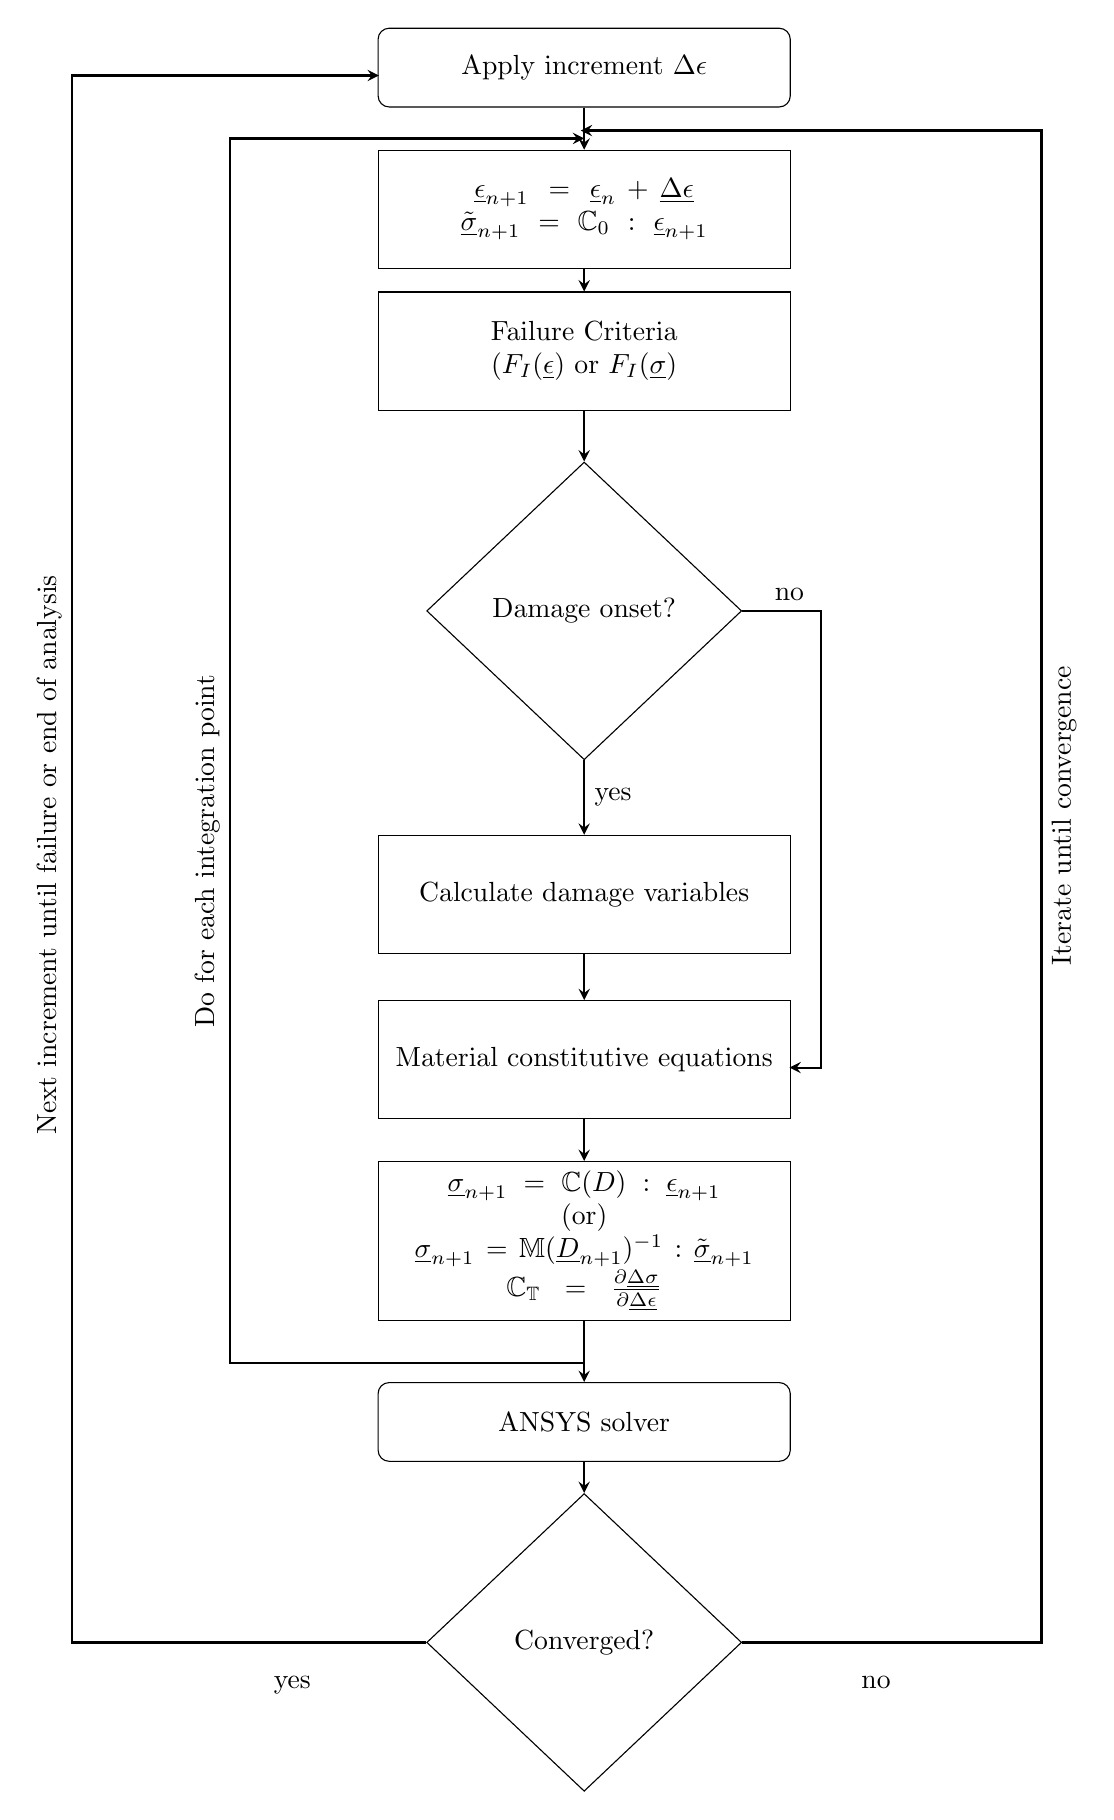
\begin{tikzpicture}[node distance = 1.8cm]

\node(straininc) [startstop] {Apply increment $\Delta\epsilon$};
\node(strainadd) [process, below of = straininc] {$\underline{\epsilon}_{n+1} = \underline{\epsilon}_{n} + \underline{\Delta\epsilon} $ \\ $\underline{\tilde{\sigma}}_{n+1} = \mathbb{C}_{0} : \underline{\epsilon}_{n+1} $};
\node(Failure)   [process, below of = strainadd] {Failure Criteria\\	 $(F_{I}(\underline{\epsilon})$ or $F_{I}(\underline{\sigma})$ };
\node(Damageon)  [decision, below of = Failure, yshift=-1.5cm] {Damage onset?};
\node(Damagecalc) [process, below of = Damageon, yshift=-1.8cm] {Calculate damage variables};
\node(Materialeqn)[process, below of = Damagecalc, yshift=-0.3cm] {Material constitutive equations};
\node(Tangent)[process, below of = Materialeqn, yshift=-0.5cm] { $\underline{\sigma}_{n+1} = \mathbb{C}(D):\underline{\epsilon}_{n + 1}$ \\ (or) \\$\underline{\sigma}_{n+1} = \mathbb{M}(\underline{D}_{n+1})^{-1}:\underline{\tilde{\sigma}}_{n+1}$ \\ $ \mathbb{C_{T}} =\frac{\partial \underline{\Delta \sigma}}{\partial \underline{\Delta \epsilon}}$};
\node(abaqus)[startstop, below of = Tangent, yshift=-0.5cm] {ANSYS solver};
\node(Converge)[decision, below of = abaqus, yshift=-1cm] {Converged?};

\draw [arrow] (straininc) -- (strainadd);
\draw [arrow] (strainadd) -- (Failure);
\draw [arrow] (Failure) -- (Damageon);
\draw [arrow] (Damageon) -- node[anchor = west]{yes} (Damagecalc);
\draw [arrow] (Damagecalc) -- (Materialeqn);
\draw [arrow] (Materialeqn) -- (Tangent);
\draw [arrow] (Tangent) -- (abaqus);
\draw [arrow] (abaqus) -- (Converge);
\draw [arrow] (Damageon.east) node[xshift=0.6cm,anchor = south]{no} -| ++(1,-5.8) -- ++(-0.4,0)  (Materialeqn);

\draw [arrow] (Converge.west)node[xshift=-1.7cm,yshift=-0.3cm,anchor = north]{yes} -| node[xshift=10cm,sloped,above]{Next increment until failure or end of analysis}++(-4.5,19.9) -- ++ (3.9,0) (straininc); 

\draw [arrow] (Converge.east)node[xshift=1.7cm,yshift=-0.3cm,anchor = north]{no} -| node[xshift=10.5cm,sloped,below]{Iterate until convergence} ++(3.8,19.2)-- ++ (-5.85,0)  (straininc); 

\draw [arrow] (0,-16.45)-|node[xshift=6.5cm,sloped,above]{Do for each integration point}++(-4.5,15.55)--(-0,-0.9);
 
\end{tikzpicture}
\end{adjustbox}
\end{center}


\newpage
\fancyhead[RE,RO]{Results and Discussion} 
\chapter{Results and Discussion}
\section{Modelling linear elastic behaviour of orthotropic materials}
\indent\indent\indent Before implementing the damage behaviour in orthotropic materials, their linear elastic behaviour must implemented which describes the phenomena before the damage initiation. As mentioned before orthtoropic materials require 9 independent material constants to model their elastic behaviour. Table (\ref{tab:Material parameters(Integration point studies}) summarises the utilised material parameters. The material parameters presented in table (\ref{tab:Material parameters(Integration point studies}) belongs to an unidirectional glass fiber-reinforced epoxy material obtained from \citep{lapczyk2007progressive}. In this material, the strength in the longitudinal direction ($X_{t}$ and $X_{c}$) is very high compared to the transverse directions ($Y_{t}$ and $Y_{c}$) because the fibers are aligned parallel to the longitudinal direction. 
\begin{figure}[htbp!]
\begin{center}
\includegraphics[width=11cm,height=8cm]{{14.Linear_SvsE.png}}
 \caption{Stress-Strain relation (Standard vs user-defined material routine)}
 \label{fig:Stress-Strain Linear elastic}
 \end{center}
\end{figure}
\FloatBarrier
\indent\indent\indent The constitutive matrix given in the section (\ref{Constitutive matrix}) and Hooke's law help us model the elastic behaviour of the orthotropic materials. The linear elastic behaviour of the orthotropic material is implemented as USERMAT in ANSYS, and in this section, the USERMAT is compared against the standard orthotropic material routine present in ANSYS using a structural example. A bar of length 10 mm and area 1 mm$^2$ (b = 1 mm, t =1 mm) fixed at one end is chosen for the analysis. The bar is constructed using 8 node SOLID 185 elements, and full integration has been used (See Figure. (\ref{fig:Mesh and BCs})) . A displacement of 1 mm is applied at the free end, and the Figure (\ref{fig:Stress-Strain Linear elastic}) compares the stress-strain relation between standard material routine and the implemented USERMAT
\begin{table}
  \begin{center}
   \resizebox{15cm}{4.8cm}{
     \begin{tabular}{l l l} 
     \hline
     \\
      \textbf{Symbol} \;\;& \textbf{Material Parameter} \;& \textbf{Value}\\
      \\
      \hline
      \\
      \vspace*{0.1cm}
      $E_{1}$ & Elastic modulus in longitudinal (1) direction &  55000e6 $N/m^{2}$\\
      \vspace*{0.1cm}
      $E_{2}$ = $E_{3}$  & Elastic modulus in transverse (2 and 3) directions   & 9500e6 $N/m^{2}$ \\
      \vspace*{0.1cm}
      $\nu_{12}$ = $\nu_{13}$  & Poisson's ratio (in-plane)  & 0.33 \\
      \vspace*{0.1cm}
      $\nu_{23}$   & Poisson's ratio (Planes 2-3)  & 0.27 \\
      \vspace*{0.1cm}
      $G_{12}$ = $G_{13}$  & In-plane shear modulus  & 5500e6 $N/m^{2}$ \\
      \vspace*{0.1cm}
      $G_{23}$   & Shear modulus (Planes 2-3)   & 3000e6 $N/m^{2}$ \\
      \vspace*{0.1cm}
      $X_{t}$ &  Tensile strength in longitudinal (1) direction  &  2500e6 $N/m^{2}$\\
      \vspace*{0.1cm}
      $X_{c}$ & Compressive strength in longitudinal (1) direction &  -2000e6 $N/m^{2}$\\
      \vspace*{0.1cm}
      $Y_{t}$ & Tensile strength in transverse (2 and 3) directions &  50e6 $N/m^{2}$\\
      \vspace*{0.1cm}
      $Y_{c}$ & Compressive strength in transverse (2 and 3) directions &  -200e6 $N/m^{2}$\\
      \vspace*{0.1cm}
      $S_{12}$ & In-plane shear strength &  50e6 $N/m^{2}$\\
       \hline
    \end{tabular}
    }
    \caption{Material parameters (Integration point studies)}
    \label{tab:Material parameters(Integration point studies}
  \end{center}
\end{table}
\FloatBarrier

\begin{figure}[htbp!]
\begin{center}
\includegraphics[width=8cm,height=5cm]{{Mesh and BCs.png}}
 \caption{Bar used for analysis: Mesh and BCs}
 \label{fig:Mesh and BCs}
 \end{center}
\end{figure}
\FloatBarrier


\begin{figure}[htbp!]
     \captionsetup[subfigure]{justification=centering}
     \begin{subfigure}[b]{0.4\textwidth}
         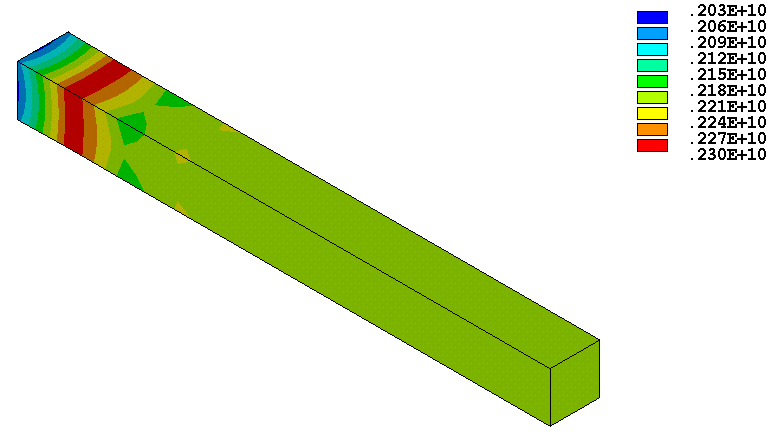
\includegraphics[width=8cm,height=5cm]{15.Ansys_SX.png}
         \caption{$\sigma_{11}$ Component of Stress}
         \label{fig:X Component of Stress}
     \end{subfigure}
     \hspace{1.85cm}
     \begin{subfigure}[b]{0.4\textwidth}
         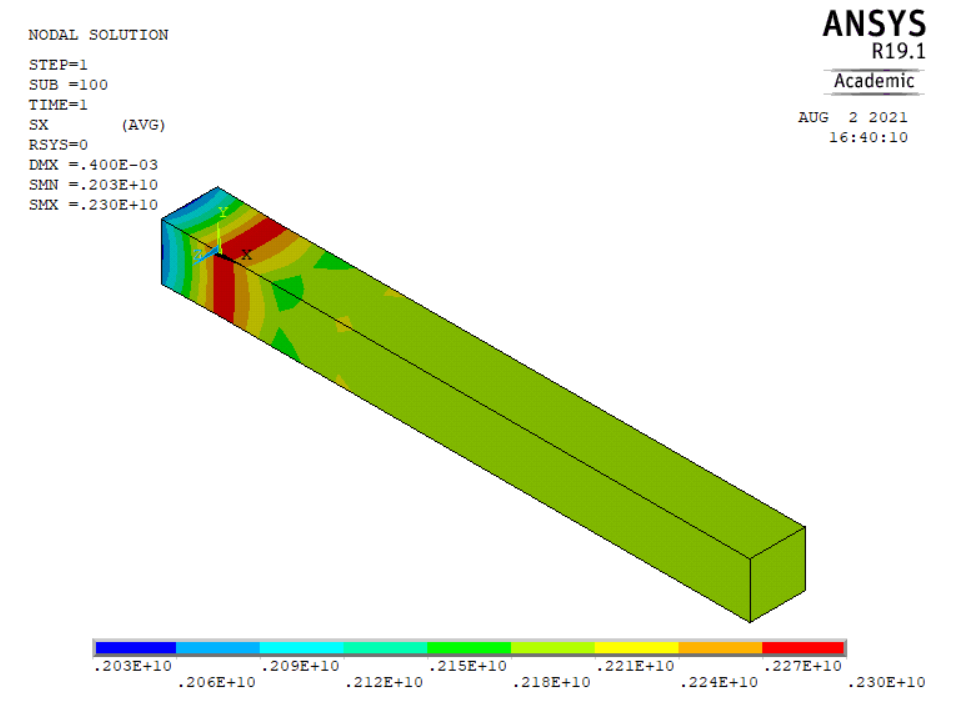
\includegraphics[width=8cm,height=5cm]{18.User_SX.png}
         \caption{$\sigma_{11}$ Component of Stress}
         \label{fig:X Component of Stress2}
     \end{subfigure}
\end{figure}
\FloatBarrier

\begin{figure}[htbp!]\ContinuedFloat     
     \begin{subfigure}[b]{0.4\textwidth}
        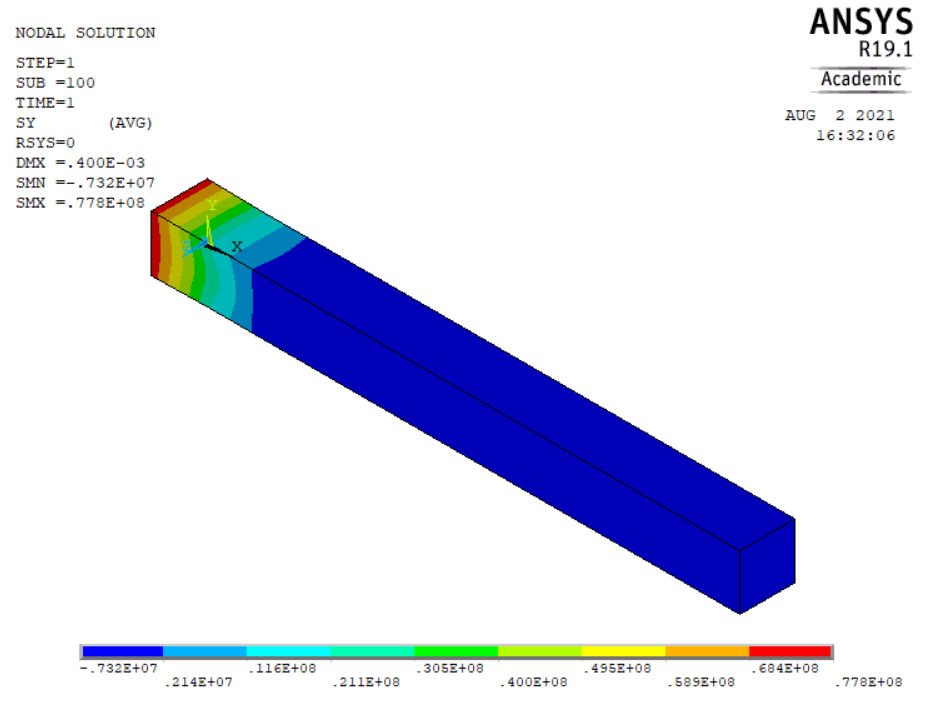
\includegraphics[width=8cm,height=5cm]{16.Ansys_SY.png}
         \caption{ $\sigma_{22}$ Component of Stress}
         \label{fig:Y Component of Stress}
     \end{subfigure}
    \hspace{1.8cm}
      \begin{subfigure}[b]{0.4\textwidth}
         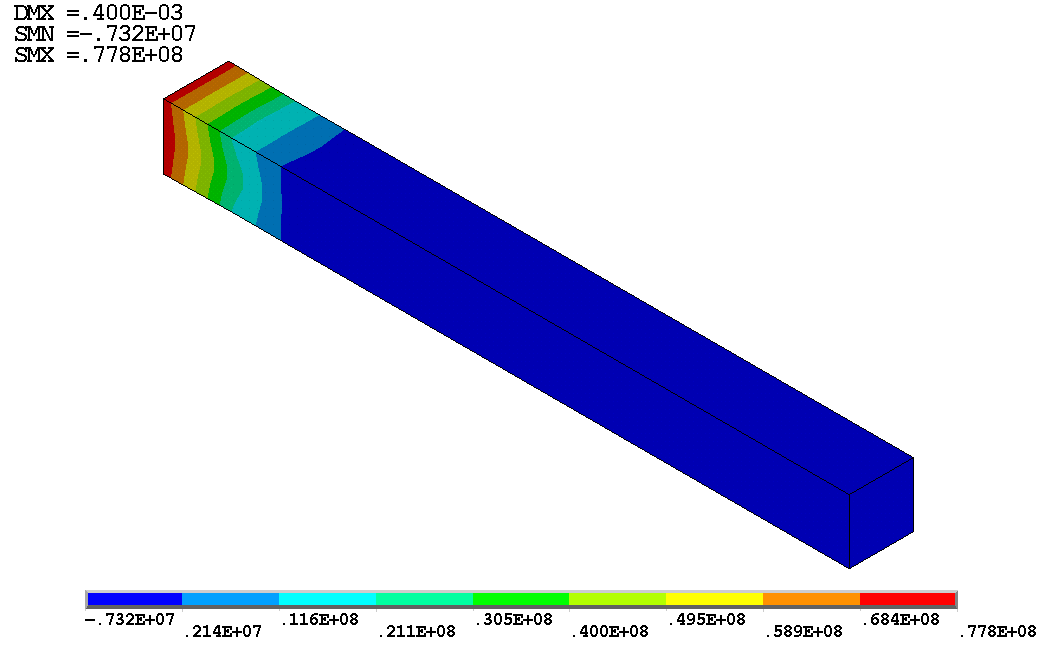
\includegraphics[width=8cm,height=5cm]{19.User_SY.png}
         \caption{ $\sigma_{22}$ Component of Stress}
         \label{fig:Y Component of Stress2}
     \end{subfigure}
\end{figure}
\FloatBarrier
\begin{figure}[htbp!]\ContinuedFloat     
     \begin{subfigure}[b]{0.4\textwidth}
         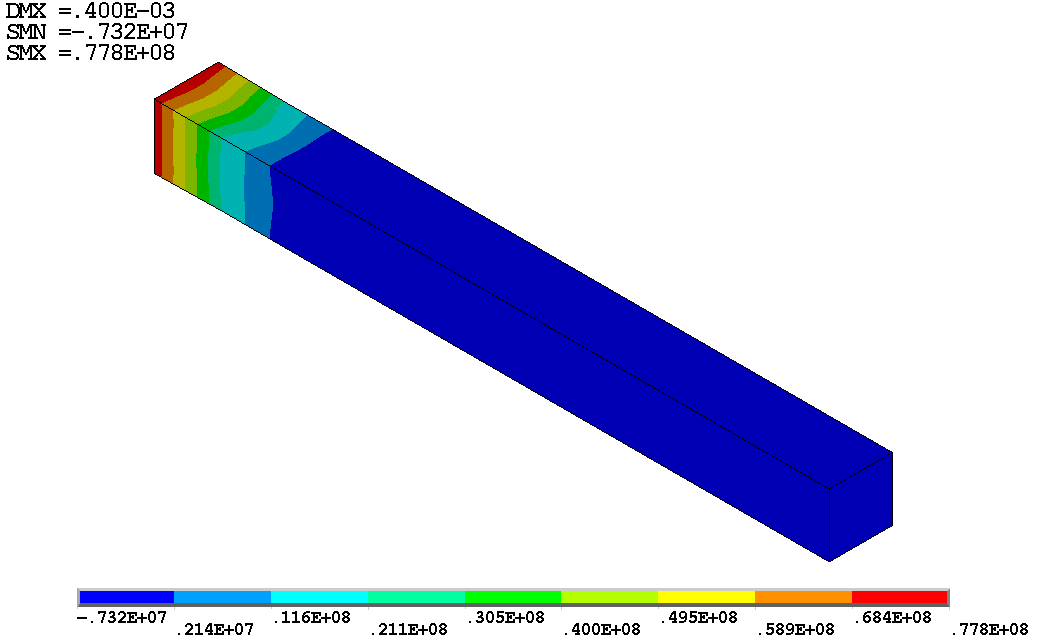
\includegraphics[width=8cm,height=5cm]{17.Ansys_SZ.png}
         \caption{$\sigma_{33}$ Component of Stress}
         \label{fig:Z Component of Stress}
     \end{subfigure}
     \hspace{1.8cm}
     \begin{subfigure}[b]{0.4\textwidth}
         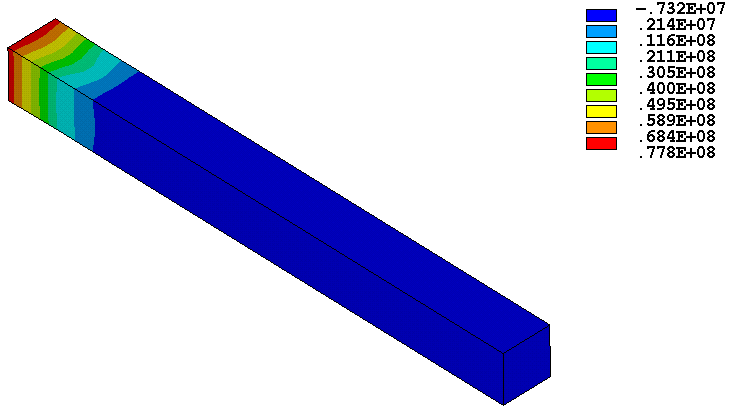
\includegraphics[width=8cm,height=5cm]{20.User_SZ.png}
         \caption{$\sigma_{33}$ Component of Stress}
         \label{fig:Z Component of Stress2}
     \end{subfigure}
        \caption{Contour plots of the stress components $\sigma_{11}$, $\sigma_{22}$ and $\sigma_{33}$ of the bar obtained using standard material routine (Figures a,c,e on the left) and  (Figures b, d, f on the right)}
        \label{fig:USERMAT}     
\end{figure}
\FloatBarrier

Figure (\ref{fig:USERMAT}) shows the contour plots of the normal stresses ($\sigma_{11}$, $\sigma_{22}$ and $\sigma_{33}$ ) computed using standard material routine and USERMAT respectively. The comparison of the stress-strain relation and contour plots between the both the routines confirm that the results obtained are similar and therefore further damage-intiation and evolution processes can now be implemented.
\section{Damage behaviour at integration point level}
\indent\indent\indent The damage models are first developed on the octave and tested using constitutive driver routines \citep{codes}, enabling us to understand the phenomenon at the integration point level. To demonstrate the evolution of damage after damage initiation and the strain-softening, following simple loading cases are investigated at the integration point level.
\begin{itemize}
\item Uniaxial tension
\item Biaxial tension
\item Triaxial tension.
\end{itemize} 
After that, the damage models are implemented as USERMAT and tested in the ANSYS environment using a 3D finite element of unit length. The finite element is subjected to the above loading cases, and the results are compared against the octave implementation
\FloatBarrier
\subsection{Uniaxial tension}
\indent\indent\indent In the case of uniaxial tension, the normal stress is present only in one direction, and all the shear stresses are zero, i.e., only one non-zero component is located on the main diagonal of the stress tensor \citep{ubt}.  In the ANSYS environment, uniaxial tension is achieved by applying a displacement on the finite element in a normal direction (e.g: longitudinal), which increases the strain $\epsilon_{11}$ linearly, and the lateral (transverse) contraction is not constrained. 3D Hashin's quadratic strain criteria (Section(\ref{3D Hashin's quadratic strain criteria })) are used to predict the damage initiation, and the exponential evolution law (Eqn.\ref{exponential damage equation}) is used to calculate the damage evolution. 
\begin{figure}[hbt!]
     \captionsetup[subfigure]{justification=centering}
      \centering
     \begin{subfigure}{0.4\textwidth}
        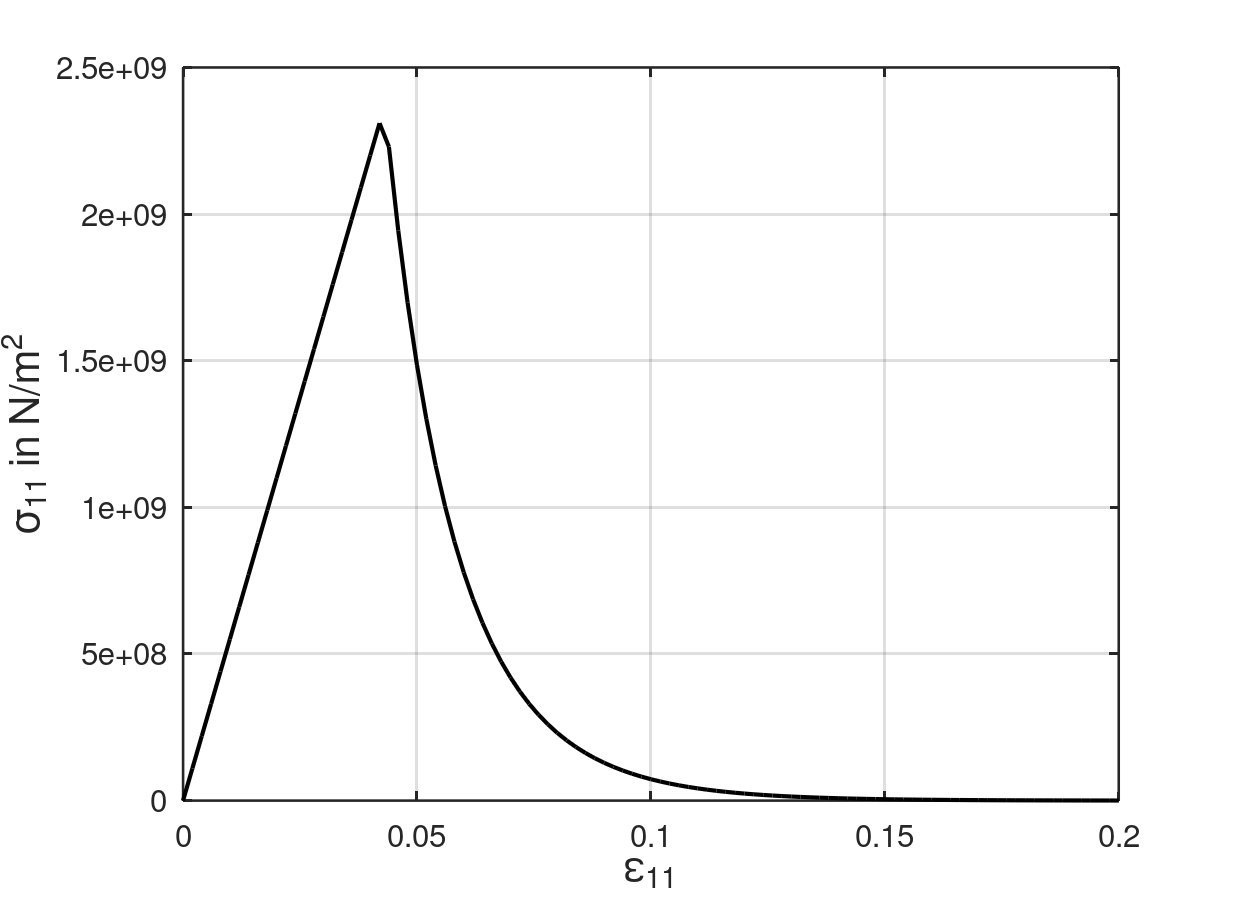
\includegraphics[width=8.3cm,height=6.35cm]{21.StressvsStrain_Ansys.png}
         \caption{$\sigma$ vs $\epsilon$ (USERMAT)}
         \label{fig:Stress-Strain relation in Ansys}
     \end{subfigure}
     \hspace{1.8cm}
     \begin{subfigure}{0.4\textwidth}
         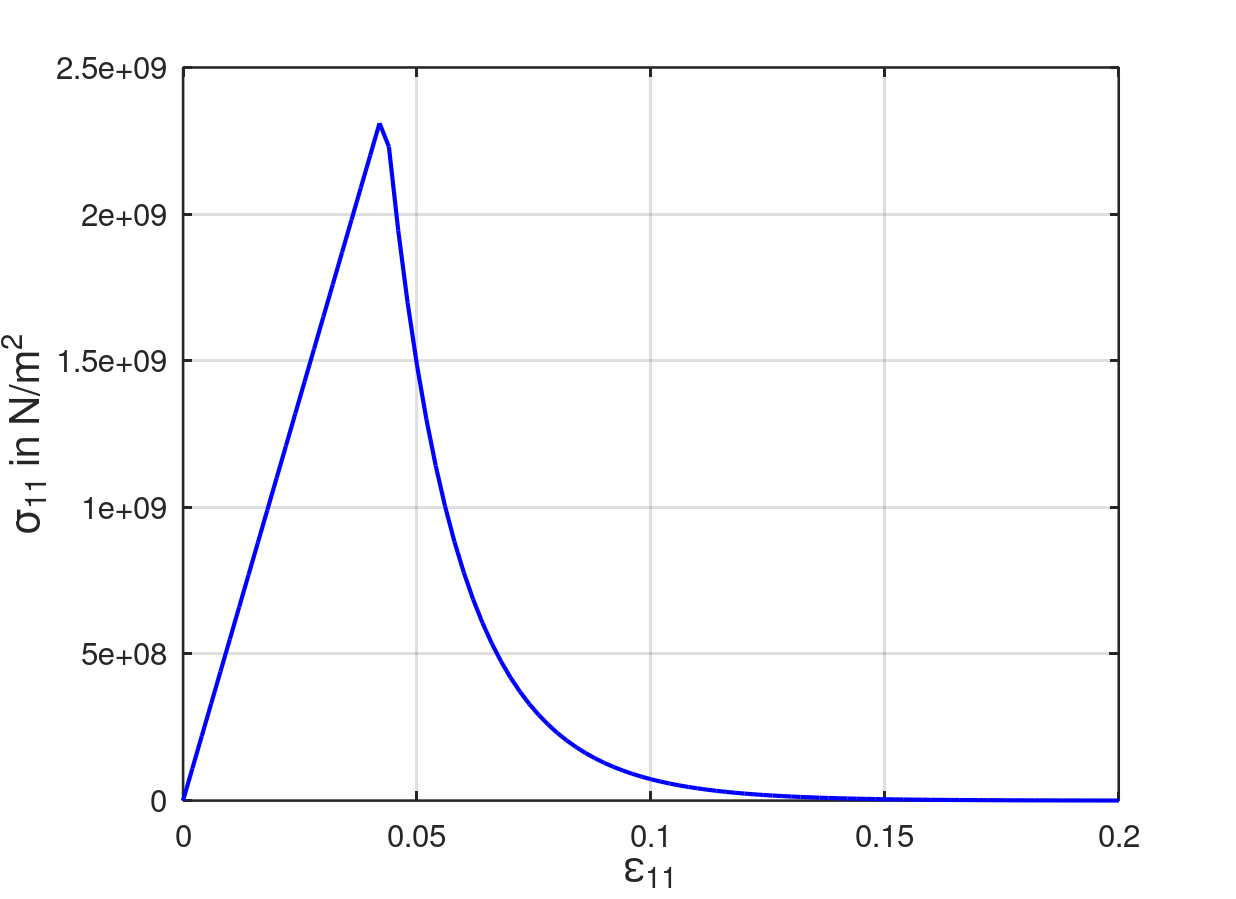
\includegraphics[width=8.3cm,height=6.35cm]{21.StressvsStrain_Octave.png}
         \caption{$\sigma$ vs $\epsilon$ (Octave)}
         \label{fig:Stress-Strain relation Octave}
     \end{subfigure}
   \caption{Evolution of stress for uniaxial tension test in 11 direction}
   \label{fig:Evolution of stress  component for a uniaxial tension test in 11 direction} 
\end{figure}
\FloatBarrier
\begin{figure}[hbt!]
\begin{center}
  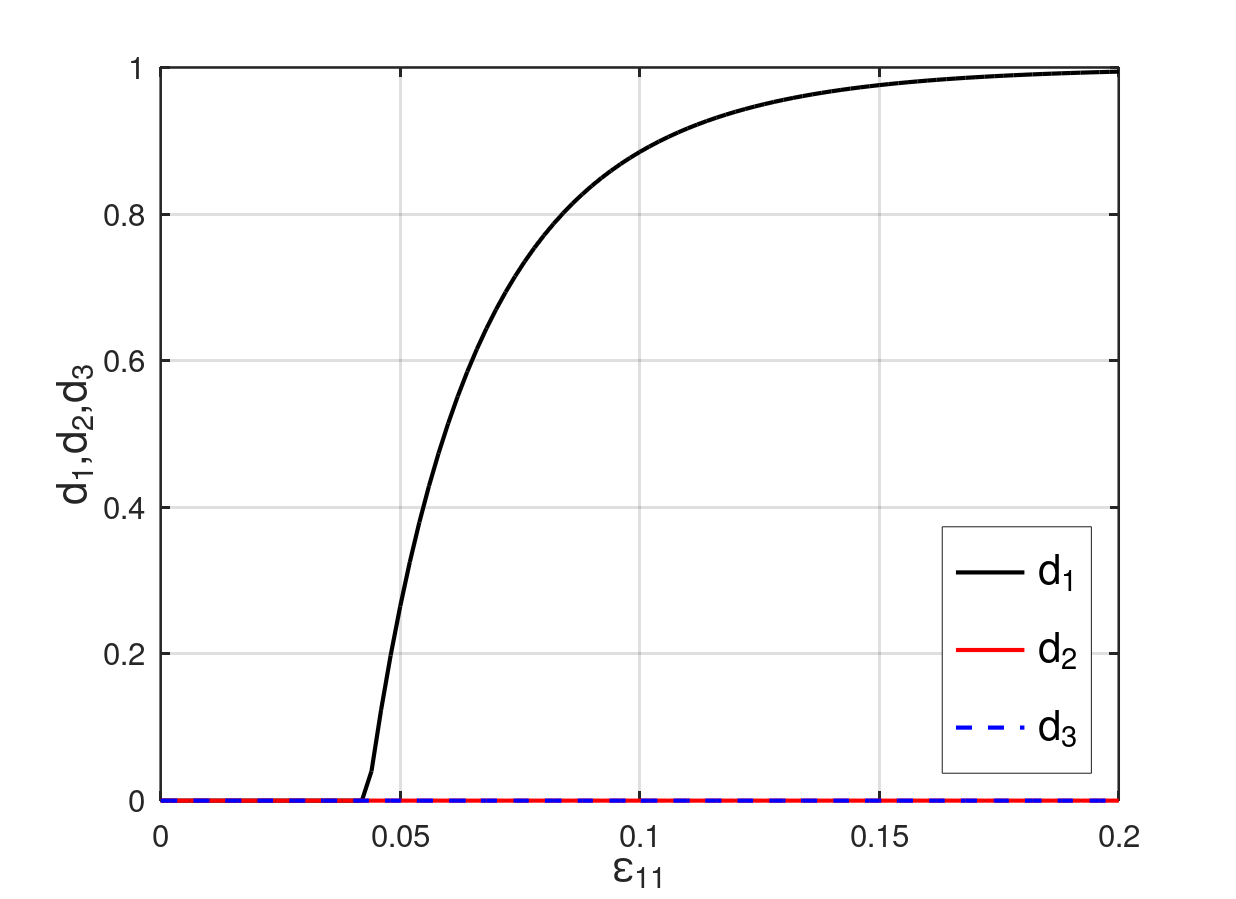
\includegraphics[width=9cm,height=6.3cm]{21.d1,d2,d3.png}
   \caption{Evolution of damage components for uniaxial tension test in 11 direction}
   \label{fig:Evolution of damage in 11 direction} 
 \end{center}    
\end{figure}
\FloatBarrier
\indent\indent\indent The stress-strain behaviour obtained from USERMAT and Octave are presented in Figure (\ref{fig:Stress-Strain relation in Ansys}) and (\ref{fig:Stress-Strain relation Octave}) respectively.  Figure (\ref{fig:Evolution of damage in 11 direction}) shows the evolution of damage variables. The system is linearly elastic until the failure strain, and the damage is zero. Once the strain $\epsilon_{11}$ exceeds the failure strain, the damage $d_{1}$ starts to evolve exponentially, and the stress starts to drop due to the reduction in stiffness in $1$ direction.  The damage variables $d_{2}$ and $d_{3}$ are zero. The comparison between the figures (\ref{fig:Stress-Strain relation in Ansys}) and (\ref{fig:Stress-Strain relation Octave}) suggests that the damage model implemented in octave and as USERMAT in ANSYS are numerically similar.


\subsubsection{Drawbacks of strain based failure criteria}
 Since the lateral contraction is not constrained during uniaxial tension, the transverse directions experience negative strain due to Poisson's effect, i.e., $\epsilon_{22}$ and $\epsilon_{33}$ will be negative. If the compressive strength in the transverse directions 2 and 3 are sufficiently low, the strains  $\epsilon_{22}$ and $\epsilon_{33}$ will exceed the failure strain. This leads to damage evolution without the presence of stress in transverse directions. 
This phenomenon cause convergence issues and the computation stops when the damage evolves without the presence of stress. Figure (\ref{fig:Convergence error}) shows the norm of the residual stress, which does not reach zero (or a below a tolerance value) after 100 iterations of the Newton-raphson, which indicates the failure of the model to converge to a solution when using low compressive strength in the transverse direction ($Y_{c}$ = -180MPa).\\
\indent\indent\indent This problem can be rectified by using stress-based failure criteria. Since damage evolution depends on failure index $F$, the transverse failure indices $F_{t}$ and $F_{z}$ will be zero during uniaxial tension if the stress-based failure criteria are used. This results in zero damage in the transverse direction. The next section presents the results obtained using stress-based damage model and the use of mesh regularization in the damage evolution law.
\begin{figure}[htbp!]
\begin{center}
\includegraphics[width=0.7\textwidth]{{22.Convergence_error.png}}
 \caption{Convergence issue: Residual norm of the stress\; $vs$ \;No of Newton-raphson iterations}
 \label{fig:Convergence error}
 \end{center}
\end{figure}
\FloatBarrier


\subsubsection{Stress-based damage models and mesh regularization}
\indent\indent\indent As mentioned in section (\ref{Mesh Regularisation}), the strain localisation problems result in strong mesh dependency, so fracture energy and characteristic length ($L_{c}$) of the element have been included in the damage evolution law in order to alleviate the problem. So the damage model is modified by changing the failure criteria to maximum stress criteria (\ref{tab:Maximum stress criterion}) and including the damage evolution equations from (\ref{d1}) to (\ref{d3}). The uniaxial tension is conducted again with the changes mentioned above and with very low transverse compression strength ($Y_{c}$ = -180MPa), and the results are presented below.
\begin{figure}[htbp!]
     \captionsetup[subfigure]{justification=centering}
     \begin{subfigure}{0.4\textwidth}
         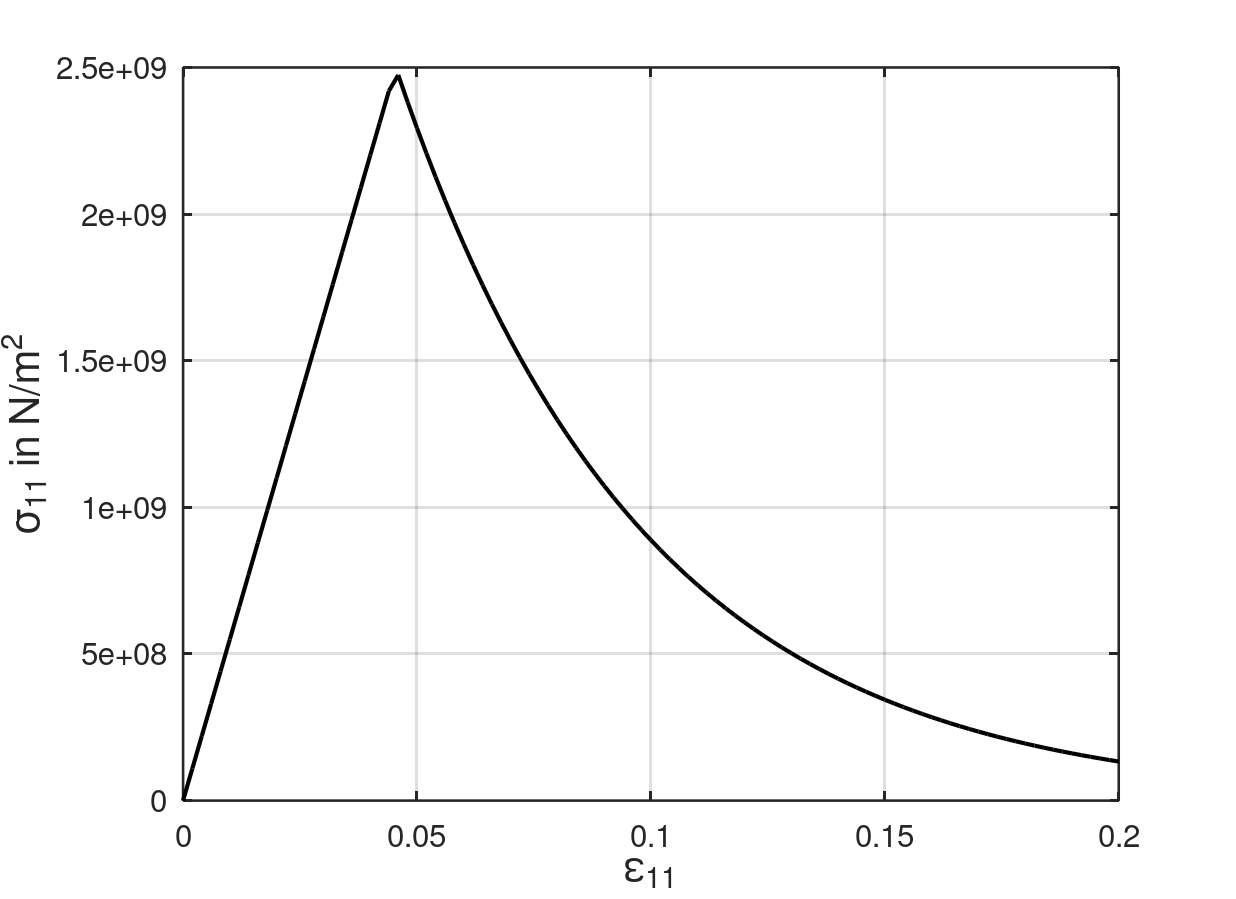
\includegraphics[width=8.3cm,height=8cm,keepaspectratio]{22.StressvsStrain_Ansys.png}
         \caption{$\sigma$ vs $\epsilon$ (USERMAT))}
         \label{fig:Stress-Strain relation in Ansys2}
     \end{subfigure}
     \hspace{1.8cm}
     \begin{subfigure}{0.4\textwidth}
          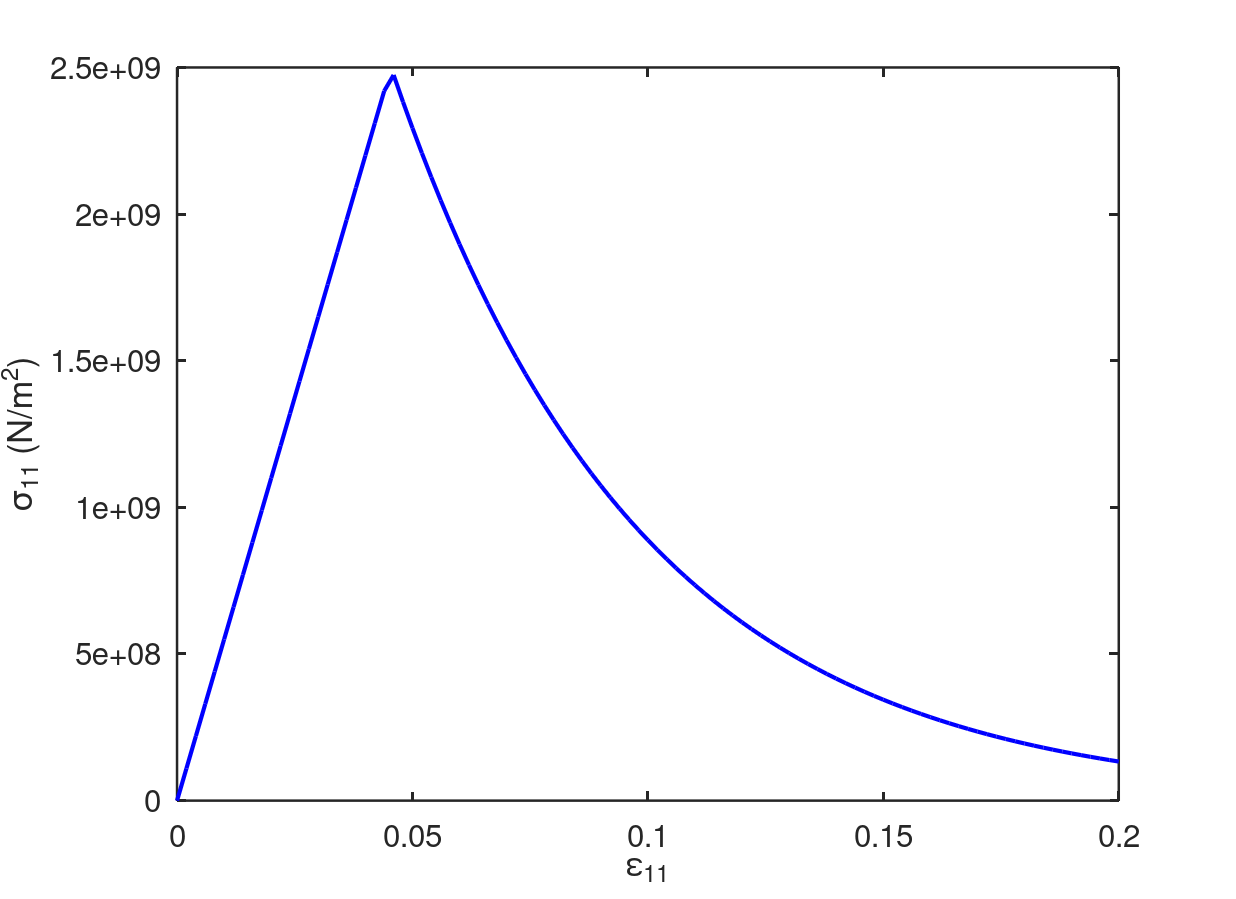
\includegraphics[width=8.3cm,height=8cm,keepaspectratio]{22.StressvsStrain_Octave.png}
         \caption{$\sigma$ vs $\epsilon$ (Octave)}
         \label{fig:Stress-Strain relation Octave2}
     \end{subfigure}
     \caption{Evolution of stress components (Stress-based damage model)}

\end{figure}
\FloatBarrier
\begin{figure}[htbp!]\ContinuedFloat
\begin{center} 
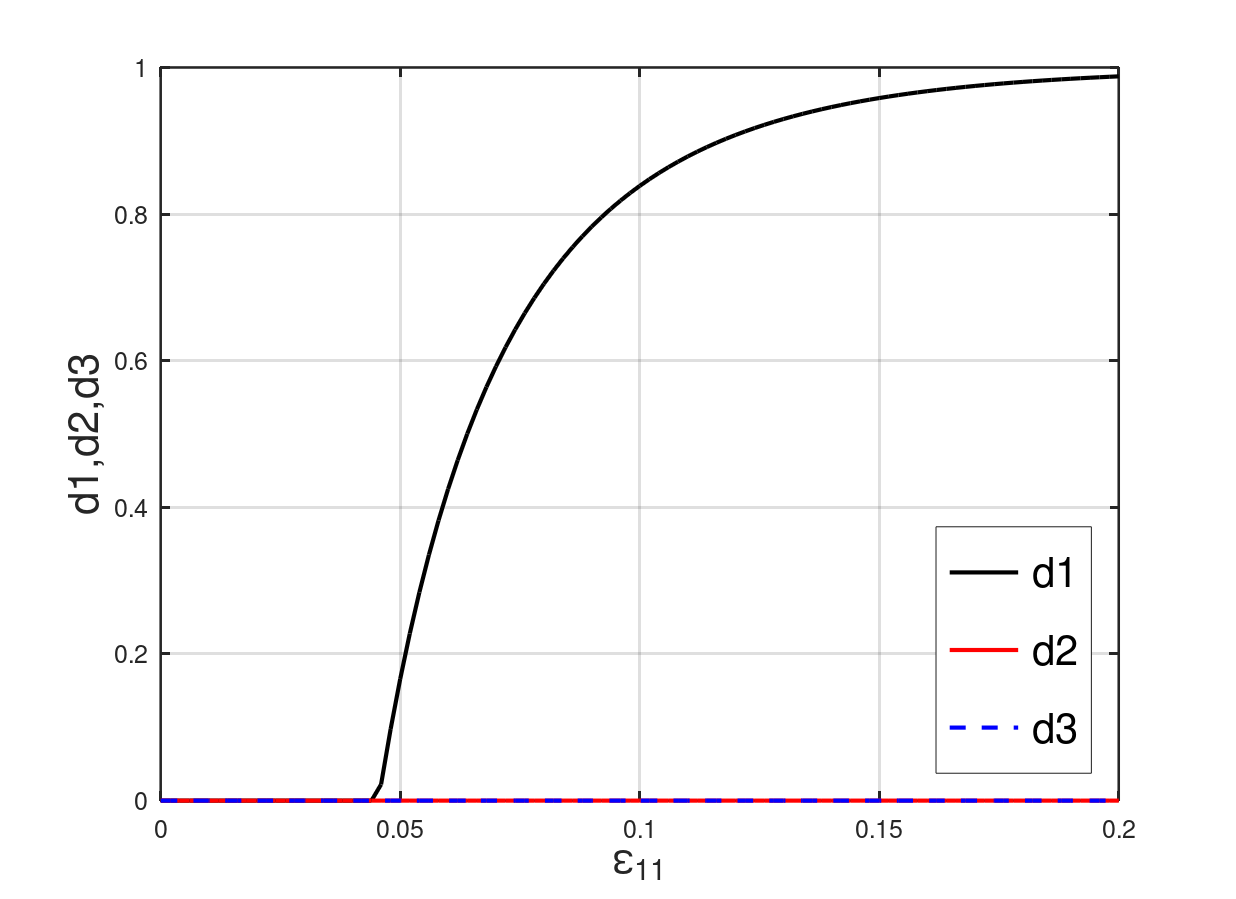
\includegraphics[width=9cm,height=6.3cm]{22.d1,d2,d3.png}
\caption{Evolution of damage components (Stress-based damage model)}
\label{fig:Evolution of stress and damage components 2} 
\end{center}    
\end{figure}
\FloatBarrier
From figure (\ref{fig:Evolution of stress and damage components 2}) it is evident that the damage  $d_{2}$ and $d_{3}$ are zero as a result of stress-based damage failure criteria because the stress components $\sigma_{22}$ and $\sigma_{33}$ are zero under uniaxial tension. While using mesh regularization, the slope of the damage curve is determined by the characteristic length ($L_{c}$), which depends on the volume of the element. The following figure (\ref{fig:Influence of element volume}) shows how the damage evolution is affected by the element volume ($V$),
\begin{figure}[htbp]
\begin{center}
\includegraphics[width=12cm,height=8.5cm]{{22.V_damage.png}}
 \caption{Influence of element volume ($V$) on the damage evolution}
 \label{fig:Influence of element volume}
 \end{center}
\end{figure}
\FloatBarrier


\subsubsection{Discussion of tangent stiffness}
\indent\indent\indent In the case of uniaxial tension, the components of the stress tensor other than $\sigma_{11}$ are zero. Since stress conditions are enforced, the octave driver routine \citep{codes} uses the Newton-raphson method to determine the input strain components other than $\epsilon_{11}$ iteratively. The Newton-raphson method requires a tangent stiffness for computation which can be derived using the equation (\ref{Anisotropic tangent stiffness}) for anisotropic damage. This enables us to test the derived algorithmic tangent stiffness (ATS) before implementing them as USERMAT in ANSYS. The derived algorithmic tangent stiffness is verified by comparing it with the numerical tangent stiffness computed using numerical perturbation. In numerical perturbation, the coefficients of the strain tensor are perturbed by a very small value, i.e.,  $\Delta\epsilon_{kl}^{n+1} = \delta$ (where $\delta<<1$) and the resulting stress perturbations are calculated \citep{codes}. 

\begin{equation}
\Delta\sigma_{ij}^{n+1} \; = \; \sigma_{ij}^{n+1}(\epsilon_{kl}^{n+1}+\delta) - \sigma_{ij}^{n+1}(\epsilon_{kl}^{n+1})
\end{equation}
Then the components of the tangent stiffness tensor can be estimated as
\begin{equation}
 C_T \;  =  \;  \frac{\Delta\sigma_{ij}^{n+1}}{\Delta\epsilon_{kl}^{n+1}}
\end{equation}
Since the material routine must be evaluated for every perturbation of $\epsilon_{kl}$ the routine has to be called six time recursively per load-step iteration. The figure (\ref{fig:Algorithmic tangent})  and (\ref{fig:Numerical perturbation}) shows the strain components $\epsilon_{22}$ and $\epsilon_{33}$ computed using algorithmic and numerical tangent stiffness which are plotted against $\epsilon_{11}$  respectively.
\begin{figure}[htbp!]
     \begin{subfigure}{0.4\textwidth}
         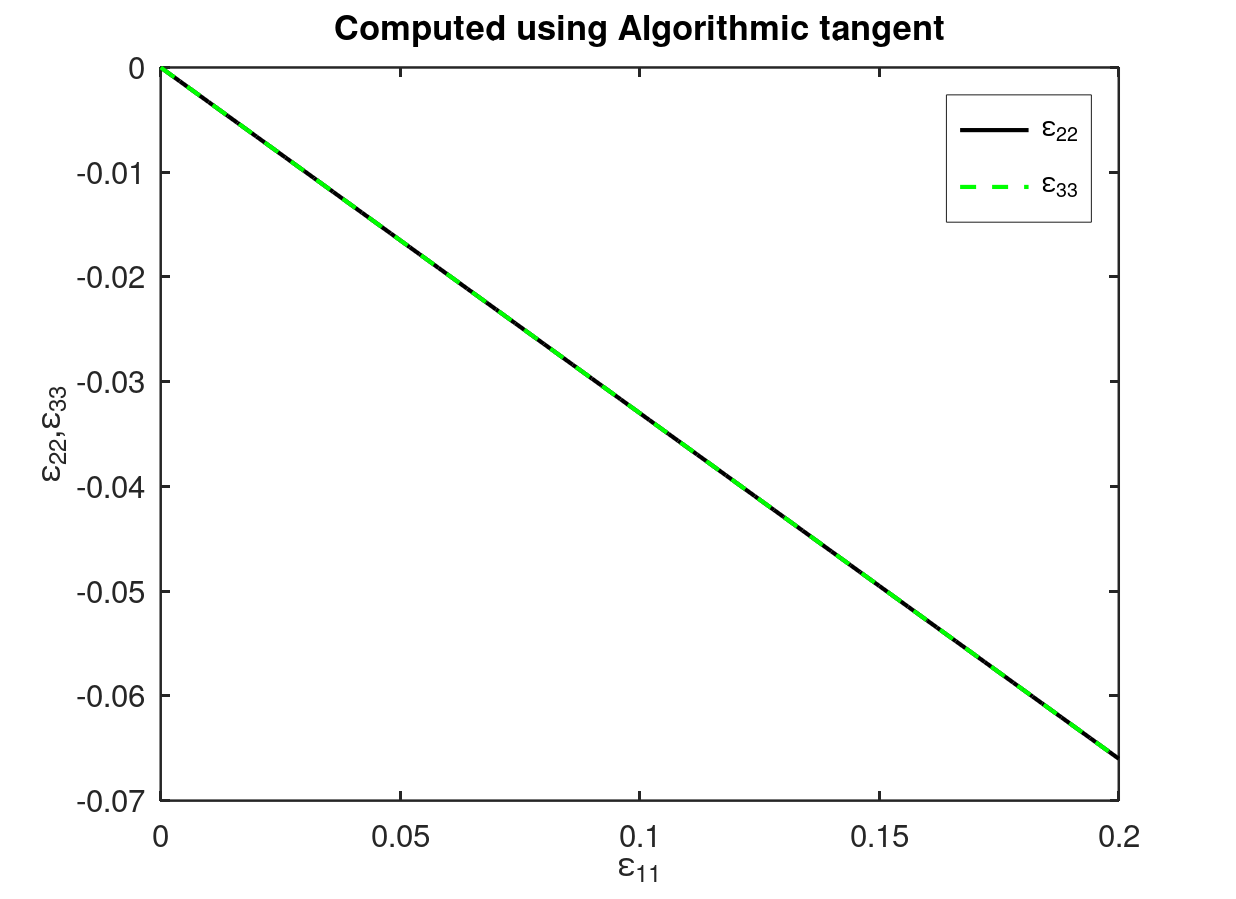
\includegraphics[width=8.3cm,height=8cm,keepaspectratio]{22.e11vse22e33_ATS.png}
         \caption{$\epsilon_{22}, \epsilon_{33}$ vs $\epsilon_{11}$ (Algorithmic tangent)}
         \label{fig:Algorithmic tangent}
     \end{subfigure}  
     \hspace{1.8cm}
     \begin{subfigure}{0.4\textwidth}
         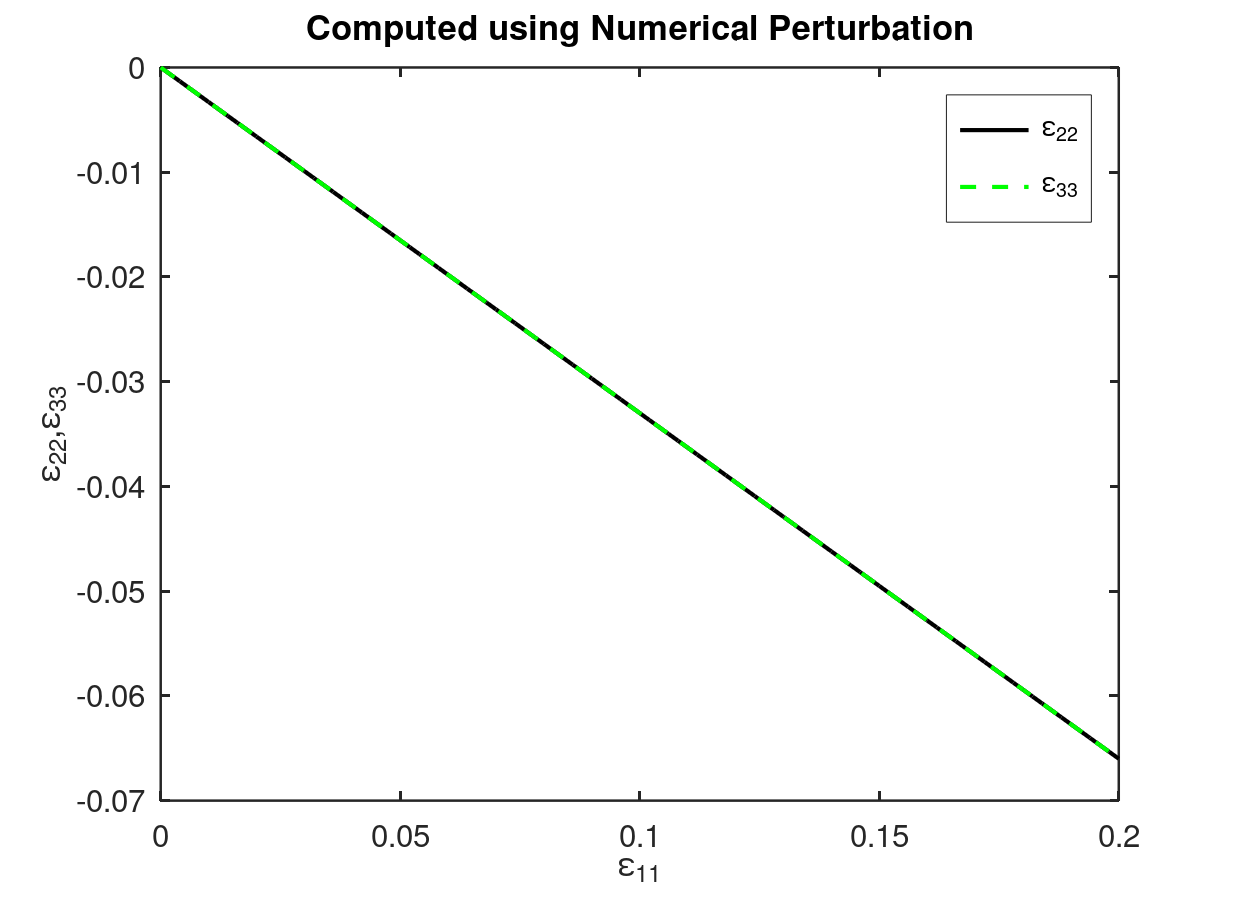
\includegraphics[width=8.3cm,height=8cm,keepaspectratio]{22.e11vse22e33_NT.png}
         \caption{$\epsilon_{22}, \epsilon_{33}$ vs $\epsilon_{11}$ (Numerical perturbation)}
         \label{fig:Numerical perturbation}
     \end{subfigure}
        \caption{The strain components $\epsilon_{22}$ and $\epsilon_{33}$ computed using algorithmic (a) and numerical tangent stiffness (b) under uniaxial tension}
        \label{fig: Algorithmic and numerical tangent stiffness under uniaxial tension}     
\end{figure}
\FloatBarrier
These comparison between above plots clearly indicates that the tangent stiffness computed using algorithmic tangent and numerical perturbation are numerically similar to each other.
\subsection{Biaxial tension}
\indent\indent\indent  In the case of biaxial tension, normal stresses are present only in two normal directions, and all the shear stresses are zero, i.e., only two non-zero components presented located on the main diagonal of the stress tensor \citep{ubt}. In ANSYS, biaxial tension is achieved by applying the same displacements in two normal directions of the finite element ($1$ and $2$ direction), and the contraction in the third direction ($3$) is unconstrained. The following figures show the corresponding stress and damage components obtained from the test.\\
\begin{figure}[hbt!]
     \captionsetup[subfigure]{justification=centering}
     \begin{subfigure}{0.4\textwidth}
         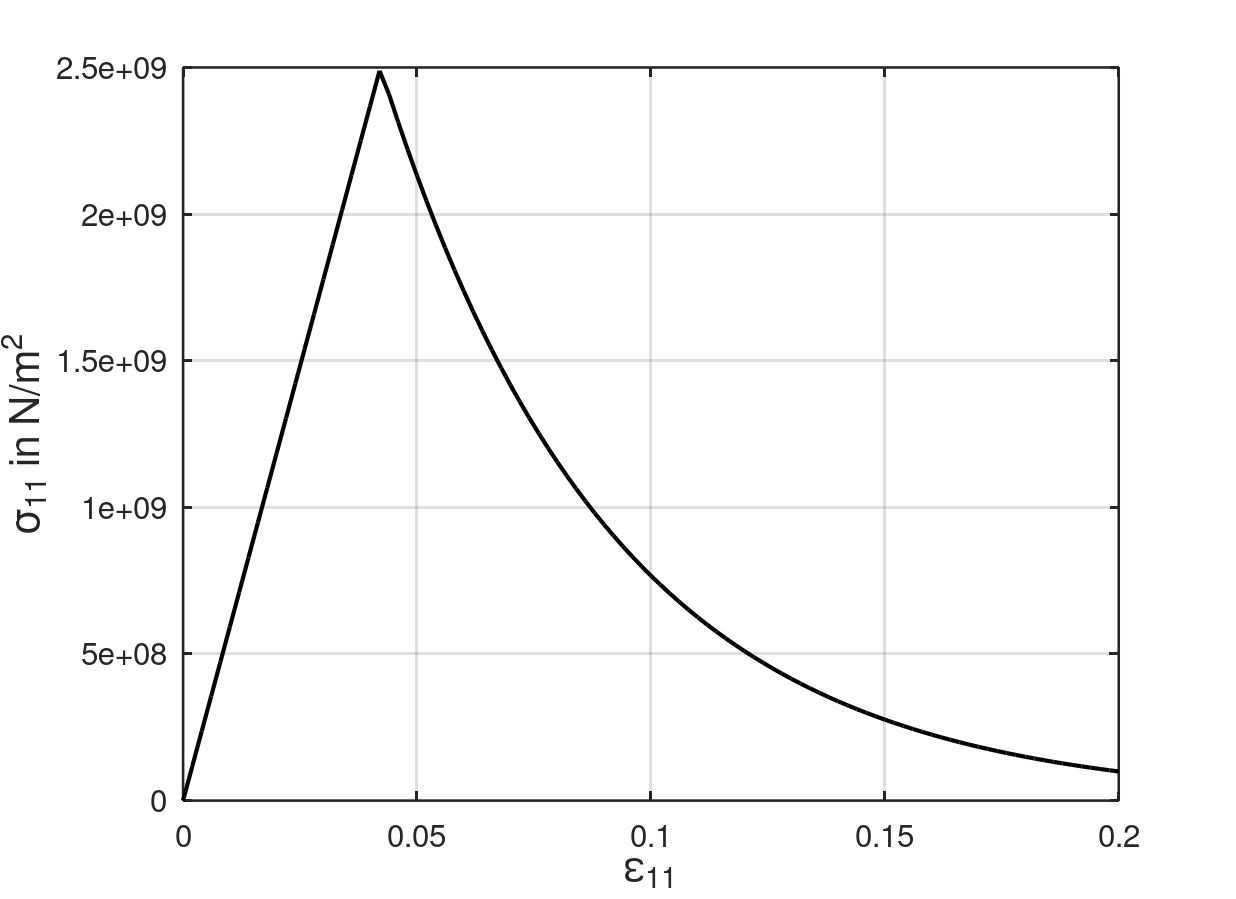
\includegraphics[width=8cm,height=8cm,keepaspectratio]{23.S11vsE11.png}
         \caption{$\sigma_{11}$ vs $\epsilon_{11}$}
         \label{fig:S11vsE11}
     \end{subfigure}
	\hspace{1.5cm}
     \captionsetup[subfigure]{justification=centering}
     \begin{subfigure}{0.4\textwidth}
         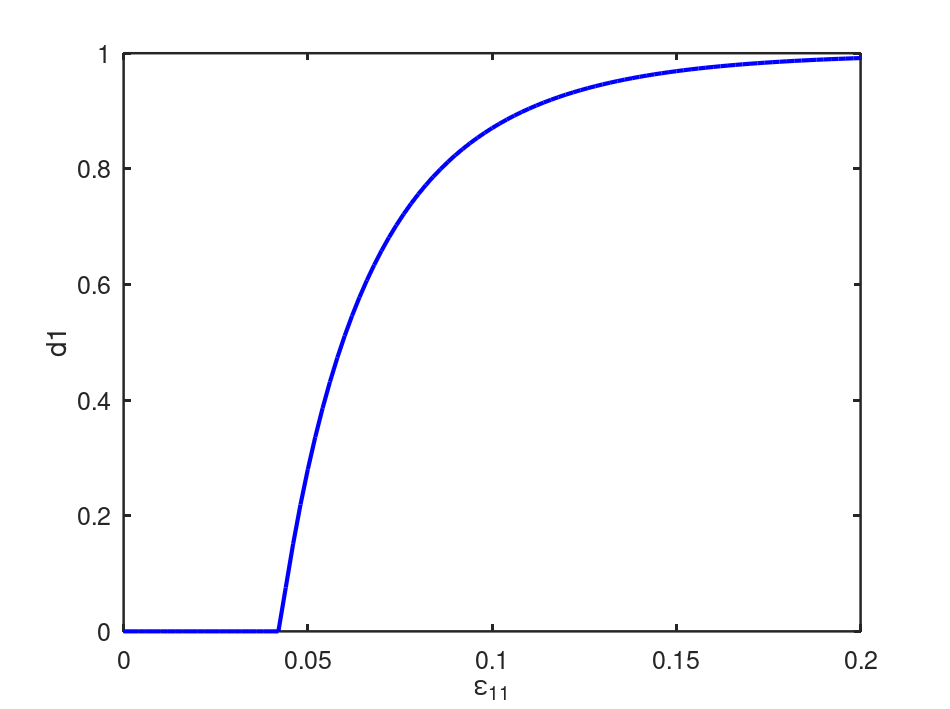
\includegraphics[width=8cm,height=8cm,keepaspectratio]{23.d1.png}
         \caption{Evolution of damage $d_{1}$}
         \label{fig:Evolution of damage d1}
     \end{subfigure}
\end{figure}
\FloatBarrier
\begin{figure}[htbp!]\ContinuedFloat 
     \begin{subfigure}{0.4\textwidth}
         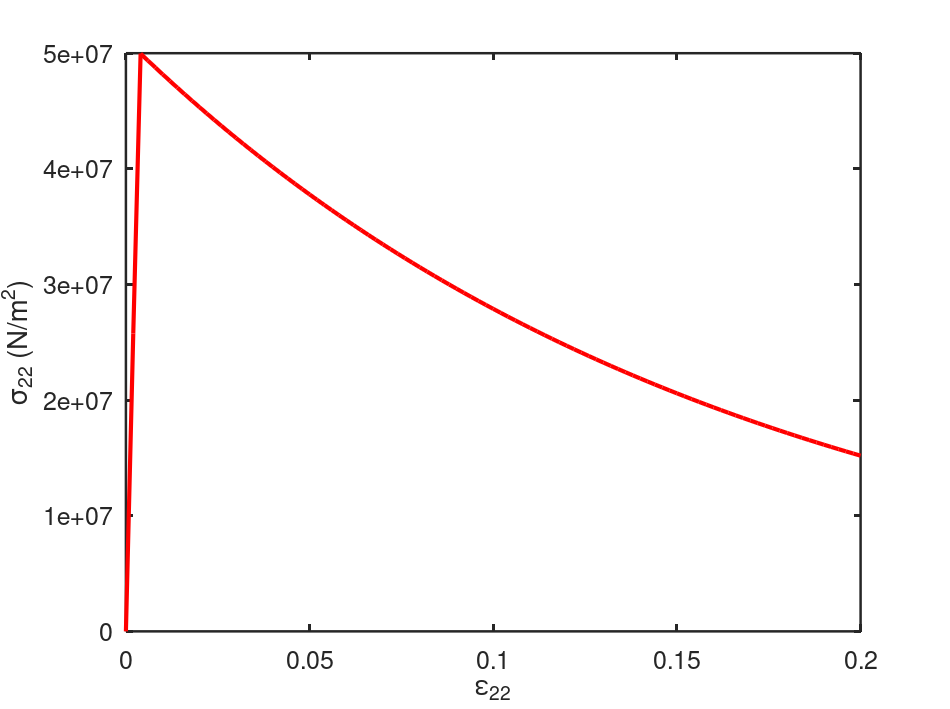
\includegraphics[width=8cm,height=8cm,keepaspectratio]{23.S22vsE22.png}
         \caption{$\sigma_{22}$ vs $\epsilon_{22}$}
         \label{fig:S22vsE22}
     \end{subfigure}
     \hspace{1.8cm}
     \begin{subfigure}{0.4\textwidth}
         \centering
         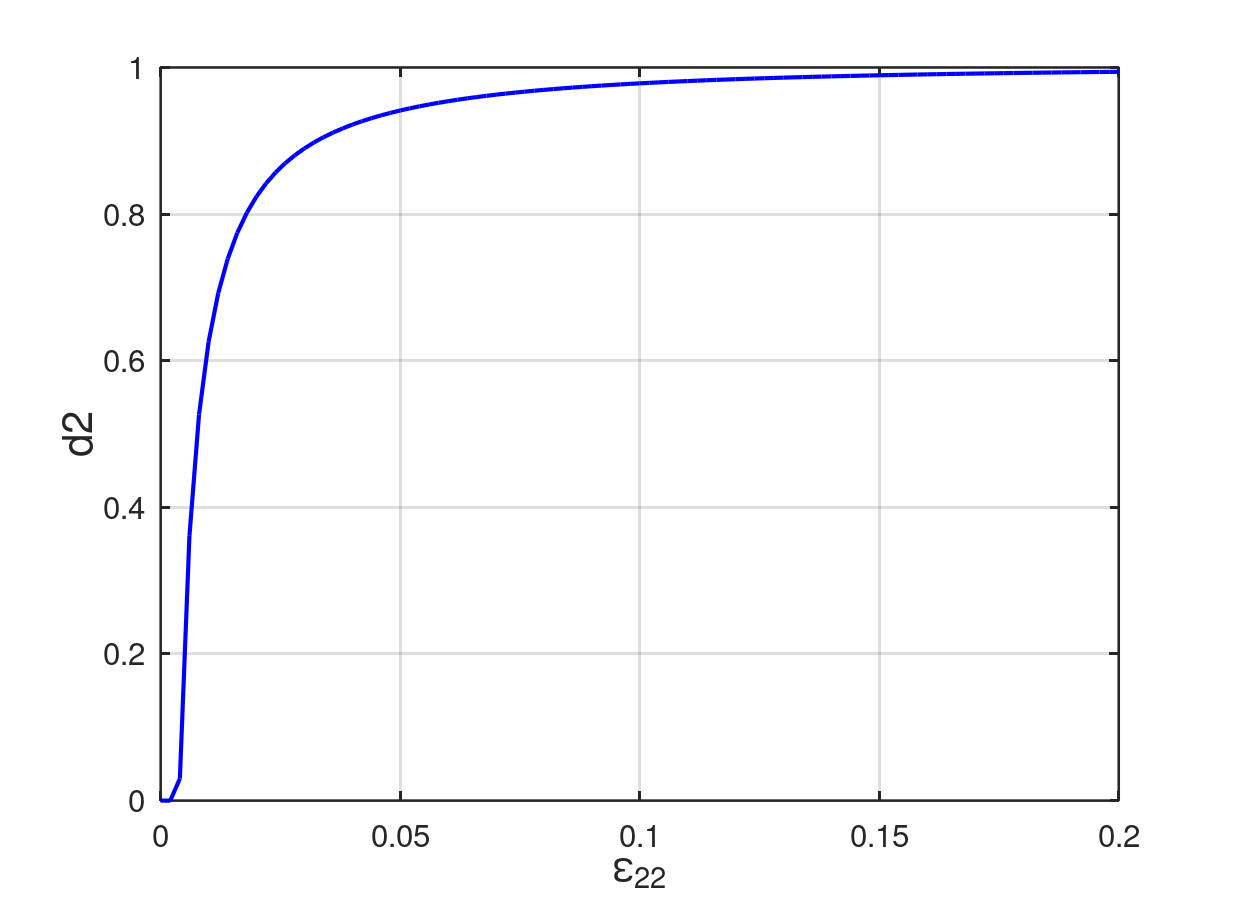
\includegraphics[width=8cm,height=8cm,keepaspectratio]{23.d2.png}
         \caption{Evolution of damage $d_{2}$}
         \label{fig:Evolution of damage d2}
     \end{subfigure}
    
        \caption{Evolution of stress (Figures a, c on the left) and corresponding damage (Figure b, d on the right) components under biaxial tension}
        \label{fig:Evolution of damage under biaxial tension}     
\end{figure} 
\FloatBarrier
Since the tensile strength in transverse direction is very low compared to the longitudinal direction, evolution of damage ($d_{2}$) begins very soon and simultaneously the stress component ($\sigma_{22}$) drops as seen in figures (\ref{fig:S22vsE22}) and (\ref{fig:Evolution of damage d2}).


\subsection{Triaxial tension}
\indent\indent\indent In the case of triaxial tension, the normal stresses are present in all three normal directions, and all the shear stresses are zero, i.e., only diagonal components of the stress tensor are non-zero.  In Ansys, triaxial tension is achieved by applying the same displacement in all three normal directions ($1$, $2$ and $3$ direction) \citep{ubt}. The following figures show the corresponding stress and damage components obtained from the test.\\

\begin{figure}[htbp!]
       \captionsetup[subfigure]{justification=centering}
     \begin{subfigure}{0.4\textwidth}
         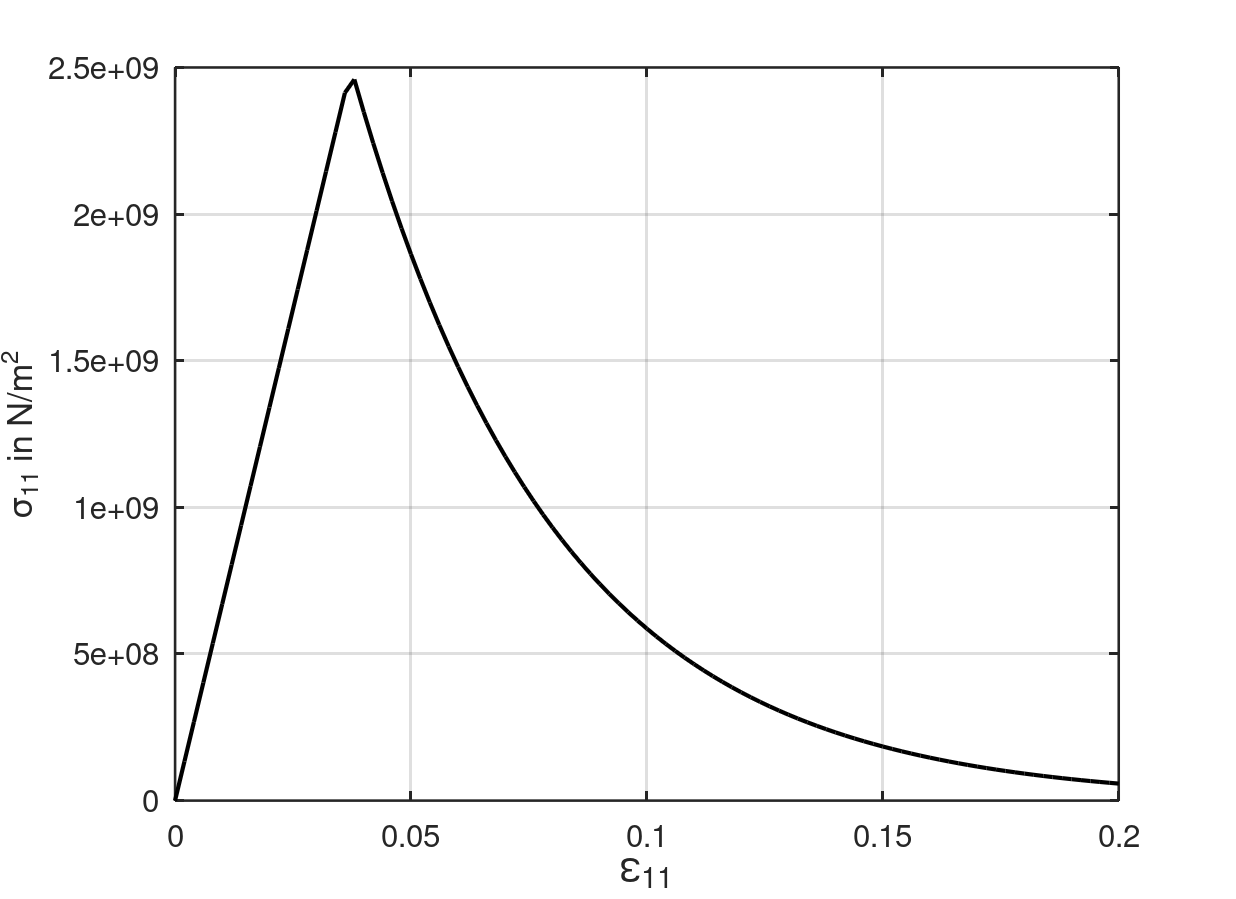
\includegraphics[width=8.5cm,height=6.5cm]{24.S11vsE11.png}
         \caption{$\sigma_{11}$ vs $\epsilon_{11}$}
         \label{fig:S11vsE11 2}
     \end{subfigure}
     \hspace{1.5cm}
     \captionsetup[subfigure]{justification=centering}
     \begin{subfigure}{0.4\textwidth}
         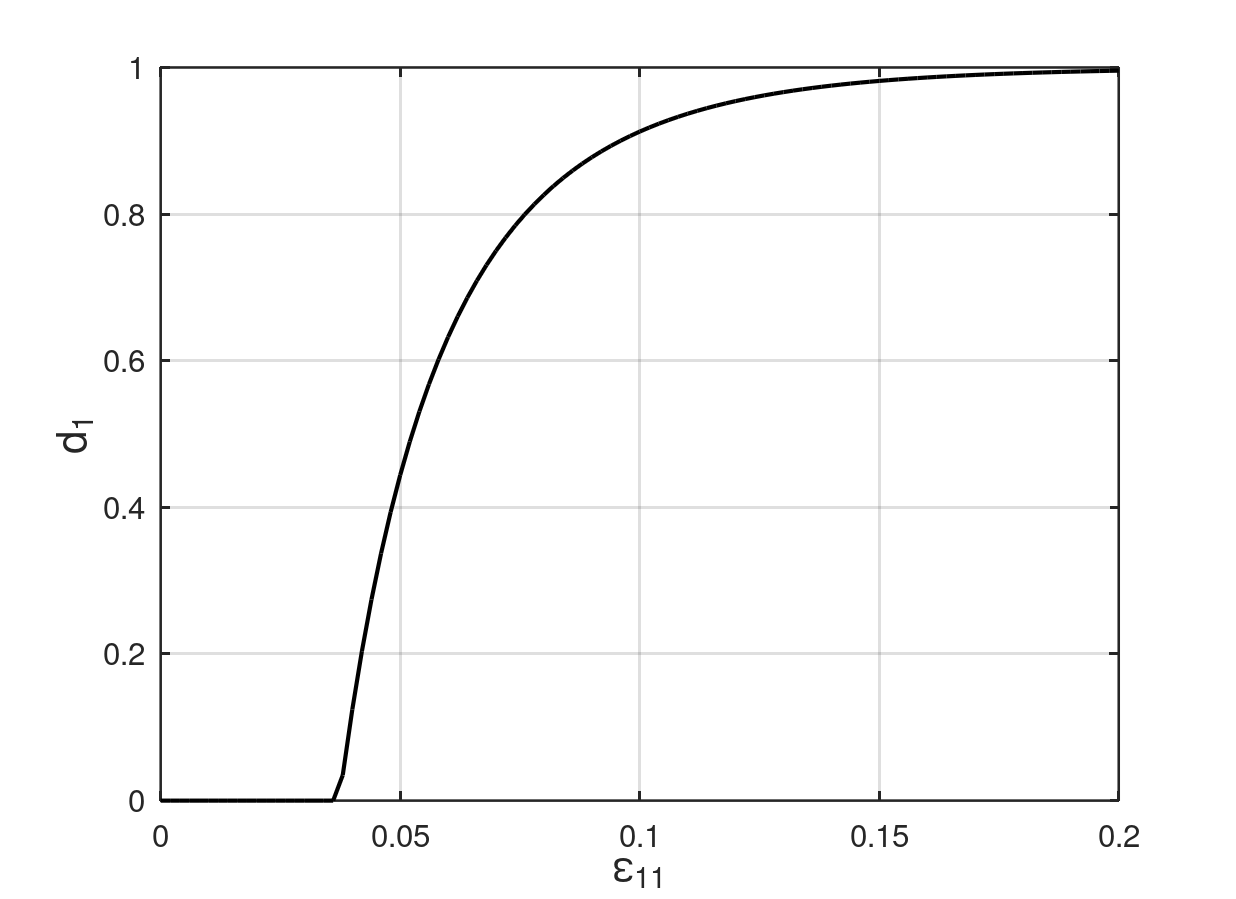
\includegraphics[width=8.5cm,height=6.5cm]{24.d1.png}
         \caption{Evolution of damage $d_{1}$}
         \label{fig:Evolution of damage d1 2}
     \end{subfigure}
\end{figure}
\FloatBarrier
\vspace*{1.8cm}
\begin{figure}[htbp!]\ContinuedFloat 
     \begin{subfigure}{0.4\textwidth}
         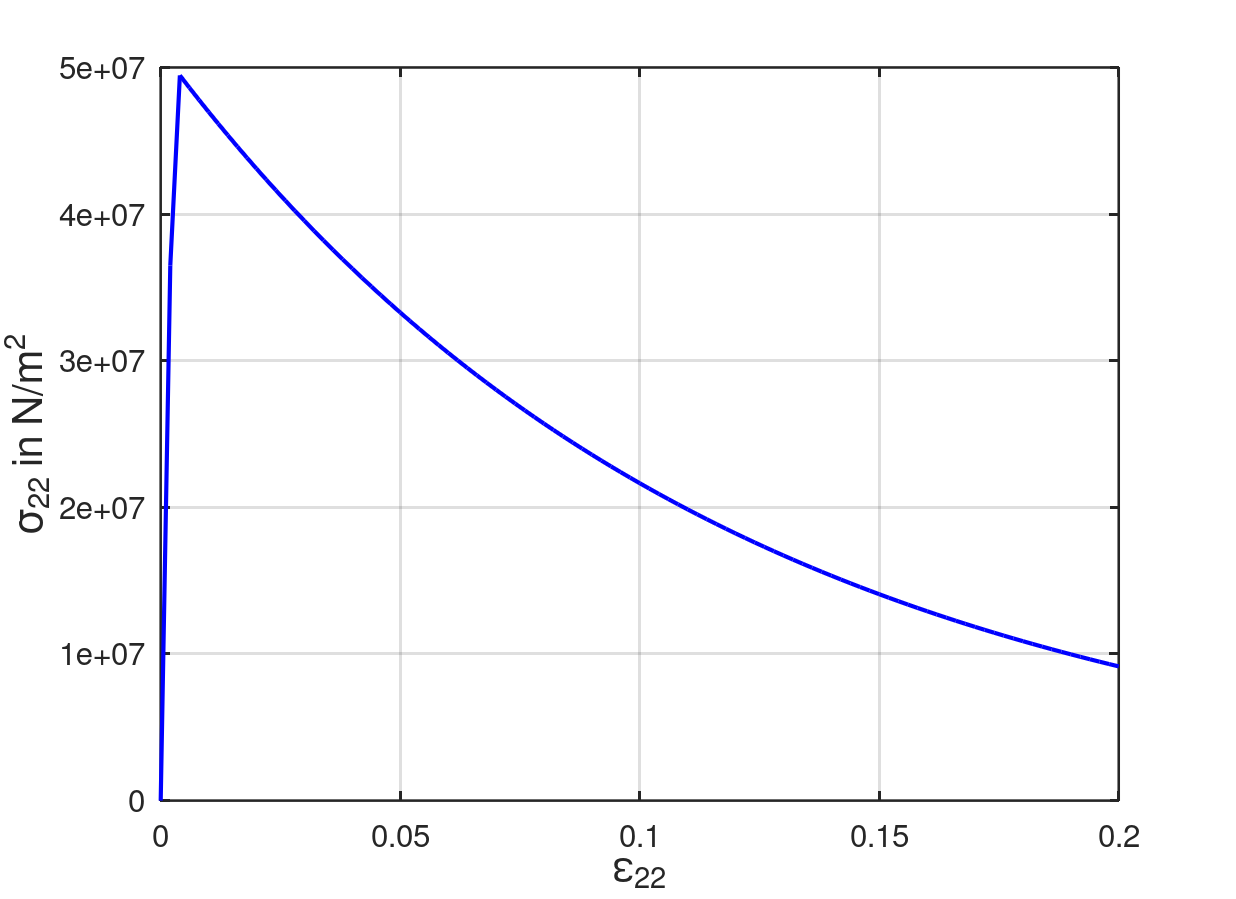
\includegraphics[width=8.5cm,height=6.5cm]{24.S22vsE22.png}
         \caption{$\sigma_{22}$ vs $\epsilon_{22}$}
         \label{fig:S22vsE22 2}
     \end{subfigure}   
     \hspace{1.5cm}
     \begin{subfigure}{0.4\textwidth}
         \centering
         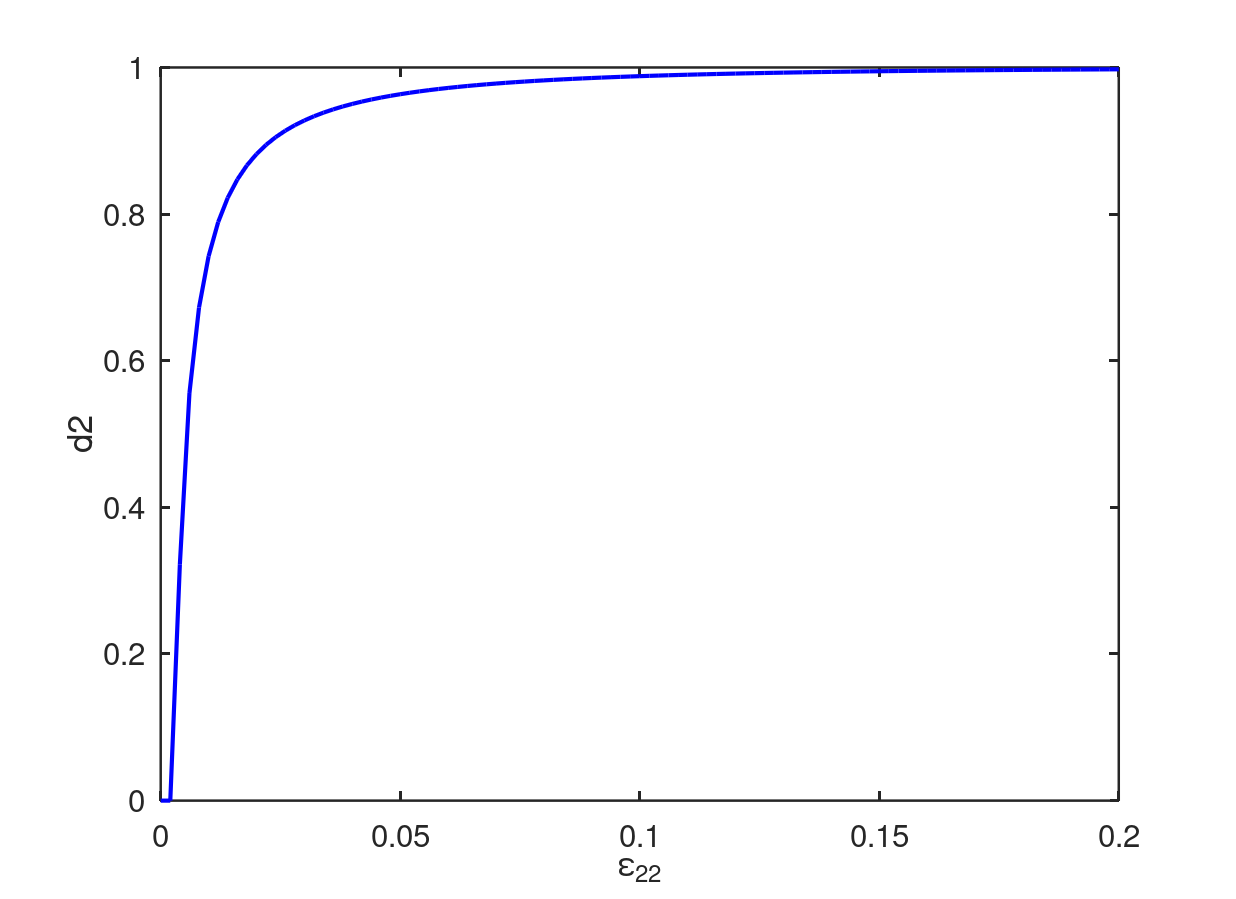
\includegraphics[width=8.5cm,height=6.5cm]{24.d2.png}
         \caption{Evolution of damage $d_{2}$}
         \label{fig:Evolution of damage d2 2}
     \end{subfigure}
\end{figure}
\FloatBarrier
\begin{figure}[htbp!]\ContinuedFloat
     \begin{subfigure}{0.4\textwidth}
         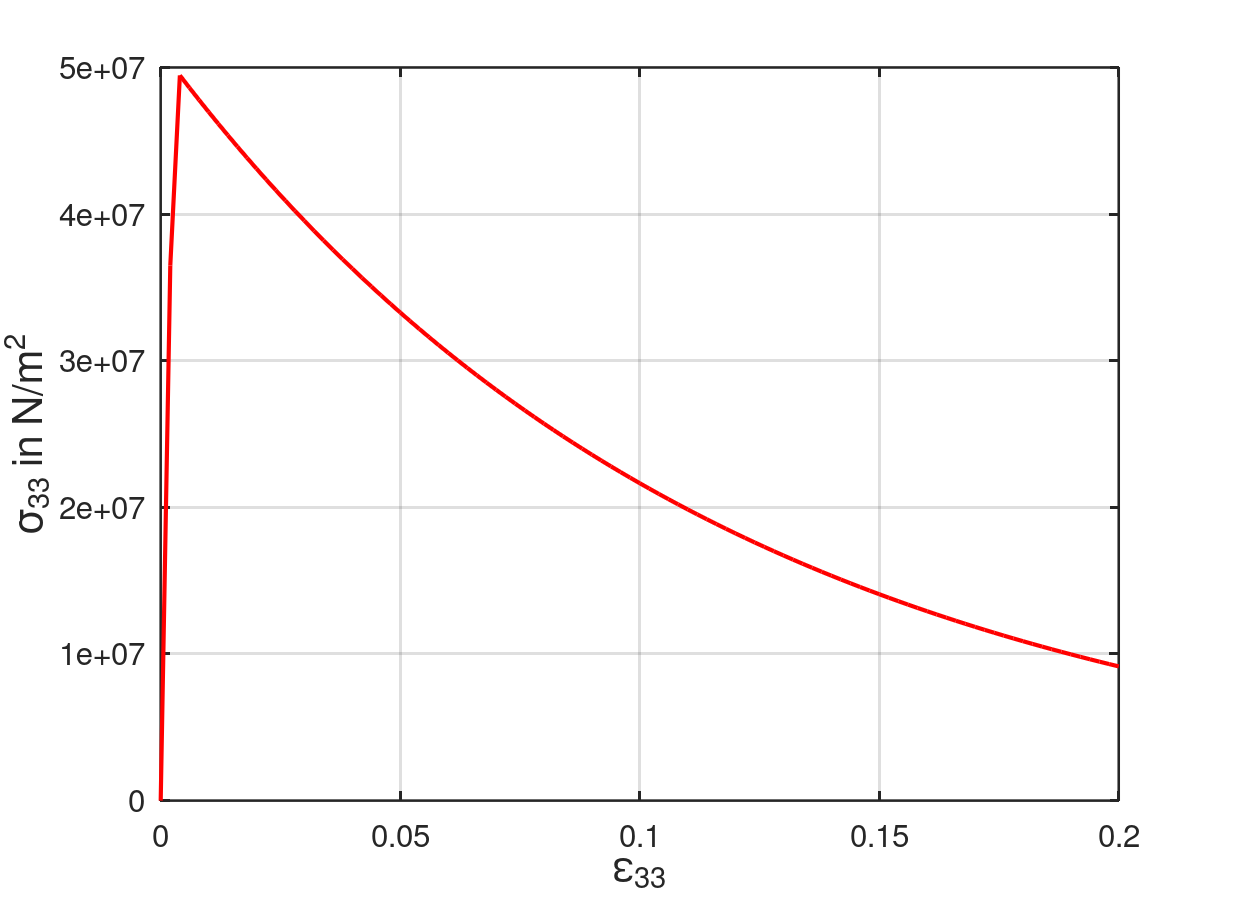
\includegraphics[width=8.5cm,height=6.5cm]{24.S33vsE33.png}
         \caption{$\sigma_{33}$ vs $\epsilon_{33}$}
         \label{fig:S33vsE33}
     \end{subfigure}
     \hspace{1.5cm}
     \begin{subfigure}{0.4\textwidth}
         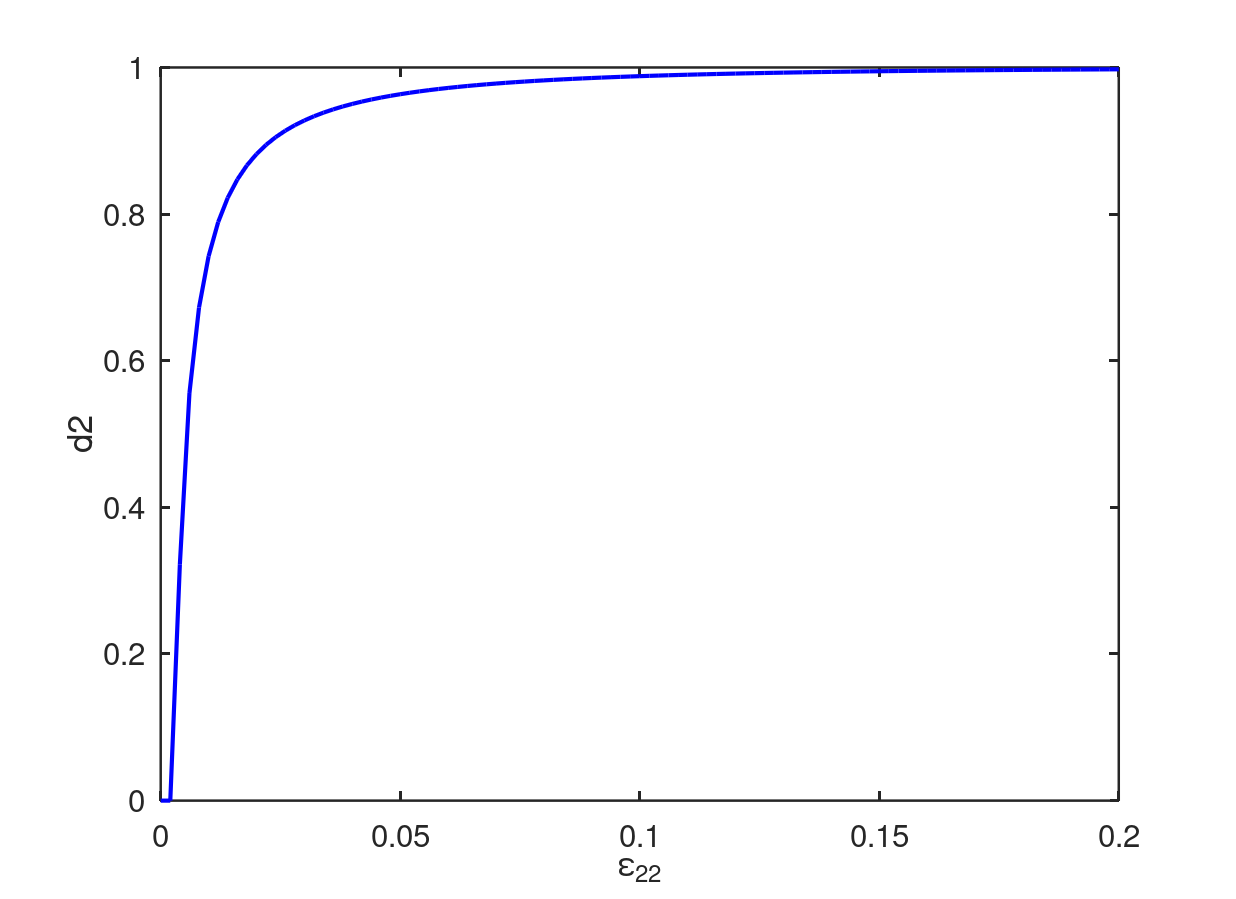
\includegraphics[width=8.5cm,height=6.5cm]{24.d2.png}
         \caption{Evolution of damage $d_{3}$}
         \label{fig:Evolution of damage d3}
     \end{subfigure}     
        \caption{Evolution of stress (Figures a, c, e on the left) and corresponding (Figures b ,d, f on the right) damage components under triaxial tension}
        \label{fig:Evolution of damage under triaxial tension}     
\end{figure}
\FloatBarrier
Since the material properties are the same in transverse $2$ and $3$ direction and the tensile strength is very low compared to the longitudinal $1$ direction, the damage $d_{2}$ and $d_{3}$ evolves simultaneously (Figure (\ref{fig:Evolution of damage d2 2}) and (\ref{fig:Evolution of damage d3})) and very soon as expected. Therefore the stress components $\sigma_{22}$ and $\sigma_{33}$ drop very soon as shown in Figure (\ref{fig:S22vsE22 2}) and (\ref{fig:S33vsE33}) 
\section{Representative structural examples}
\indent\indent\indent The following structural examples are used to test the damage model implemented as a USERMAT in the ANSYS environment
\begin{itemize}
\item Notched tensile specimen (2D - Plane stress)
\item Compact tension (CT) specimen (2D - Plane stress)
\item Plate with hole (3D)
\end{itemize}
Each example is chosen to demonstrate specific features of the damage model. These features include, at first, the capability of the model to represent damage initiation and propagation and secondly, the calculation of multiple damage variables, i.e., the ability to show anisotropic damage development in the composite material when a load is applied, both in 2D and 3D setting. Furthermore, mesh convergence studies are performed to show that the regularization scheme employed gives better results than the model with no regularization. For all the finite element simulations of the above models, linear quadrilateral elements are used (both 2D and 3D) with full Gauss integration. The line search option has been enabled during all the simulations to get good convergence behaviour. The material used for the finite element simulations is T700/2510 carbon fiber/epoxy fabric. The material has fibers in parallel in the longitudinal direction and also fibers woven in the cross-section that provide additional strength in transverse directions. The material has a high modulus and strength in the longitudinal direction compared to the transverse direction. The material properties are obtained from \citep{jiang2018evaluations} and a summary of the material properties are given in the Table (\ref{tab:Material parameters(Representative structural examples)}). \\
\begin{table}[!htbp]
  \begin{center}
    
\resizebox{16cm}{6.5cm}{ 
     \begin{tabular}{l l l} 
     \hline
     \\
      \textbf{Symbol} \;\;& \textbf{Material Parameter} \;& \textbf{Value}\\
      \\
      \hline
      \\
      \vspace*{0.1cm}
      $E_{11}$ & Modulus in longitudinal (1) direction &  55.8 GPa\\
      \vspace*{0.1cm}
      $E_{22}$ = $E_{33}$  & Modulus in transverse (2 and 3) directions   & 54.9 GPa \\
      \vspace*{0.1cm}
      $\nu_{12}$ & Poisson's ratio   & 0.043 \\
      \vspace*{0.1cm}
      $G_{12}$ =  $G_{23}$ = $G_{13}$   &  Shear modulus  & 4.2 GPa \\
      \vspace*{0.1cm}
      $X_{t}$ &  Tensile strength in longitudinal (1) direction & 910.1 MPa\\
      \vspace*{0.1cm}
      $X_{c}$ & Compressive strength in longitudinal (1) direction & -710.2 MPa\\
      \vspace*{0.1cm}
      $Y_{t}$ & Tensile strength in (2 and 3) directions  & 772.2 MPa\\
      \vspace*{0.1cm}
      $Y_{c}$ & Compressive strength in (2 and 3) directions &  -703.3 MPa\\
      \vspace*{0.1cm}
      $S_{12}$ & In-plane strength &  131 MPa\\
      \vspace*{0.1cm}
      $G_{f}^{lt}$ & Tensile fracture energy along longitudinal (1) direction  &  125 KJ/$m^{2}$\\
      \vspace*{0.1cm}
      $G_{f}^{lc}$ & Compressive fracture energy along longitudinal (1) direction  &  250 KJ/$m^{2}$\\
      \vspace*{0.1cm}
      $G_{f}^{tt}$ & Tensile fracture energy along (2 and 3) directions   &  95 KJ/$m^{2}$\\
      \vspace*{0.1cm}
      $G_{f}^{tc}$ & Compressive fracture energy along (2 and 3) directions  & 254 KJ/$m^{2}$\\
      \\
       \hline
    \end{tabular}
    }
     \\
    \caption{Material parameters (Representative structural examples)}
    \label{tab:Material parameters(Representative structural examples)}
  \end{center}
\end{table}
\FloatBarrier
\clearpage
\subsection{Notched tensile specimen}
\indent\indent\indent  The first example demonstrates the model's capability to represent damage initiation and propagation. A notched tensile specimen is widely used for analysis of stress concentration, fatigue etc., Because of the symmetry, only one-quarter of the specimen is modelled in the finite element analysis and the geometry and boundary conditions are shown in the Figure (\ref{fig:NT Specimen}). The meshes consist of plane-stress elements (PLANE 182) with bilinear interpolations for displacements, and 2*2 Gauss integration has been utilized. Three different finite element meshes have been used in the fracture zone with the elements of h = 1 mm, 0.5 mm, 0.25 mm and a total of 500, 840, 1460 elements respectively for the convergence studies (Figure \ref{fig:Considered meshes}).  At first, the longitudinal direction is kept parallel to the loading direction, and the behaviour of the model is analyzed by applying a displacement controlled load ($U_{x}$) in the longitudinal direction (X-direction). The maximum stress criterion (Section \ref{Maximum stress criteria}) has been used to predict the damage initiation.

\begin{figure}[htbp!]
\begin{center}
\includegraphics[width=0.6\textwidth]{{25.Geometry.jpg}}
 \caption{Specimen geometry and boundary conditions. Dimensions are given in mm. Displacement controlled loading $U_{x}$ is applied.}
 \label{fig:NT Specimen}
 \end{center}
\end{figure}
\FloatBarrier
\indent\indent\indent   The force-displacement response for the three different meshes with and without the regularization (Section(\ref{Mesh Regularisation})) schemes have been plotted in Figure (\ref{fig:with regularization})  and (\ref{fig:without regularization}) respectively. The global force-displacement response is characterized by a large linear regime followed by a gradual drop of the load (because of the softening) or a sudden drop in case of no regularization. From Figure (\ref{fig:Convergence study}), it is clearly evident that the model with regularization gives a more stable force-displacement response compared to the model without regularization, where the maximum load capacity is very low, and the load drops significantly with the decrease in mesh size (i.e., increase in the number of elements). The regularization scheme employed cannot fully alleviate the mesh dependency problem because the damage evolution is still dependent on the element volume ($V$) discussed in the Figure. (\ref{fig:Influence of element volume}). But it improves the solution significantly compared to the material model without regularization. 

\begin{figure}[htbp!]
     \captionsetup[subfigure]{justification=centering}
     \begin{subfigure}{0.27\textwidth}
         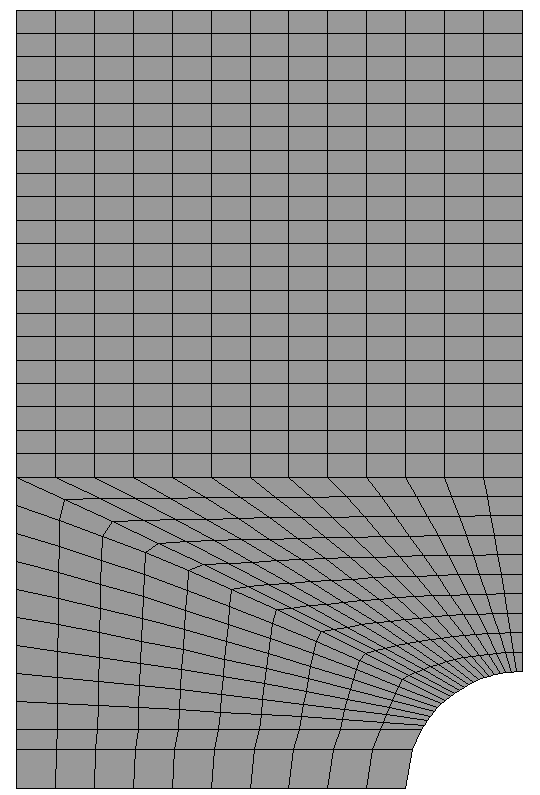
\includegraphics[width=1.19\textwidth]{25.1mm2.png}
         \caption{h=1 mm, n=500 elements}
         \label{fig:1mm}
     \end{subfigure}
     \hfill
     \begin{subfigure}{0.27\textwidth}
         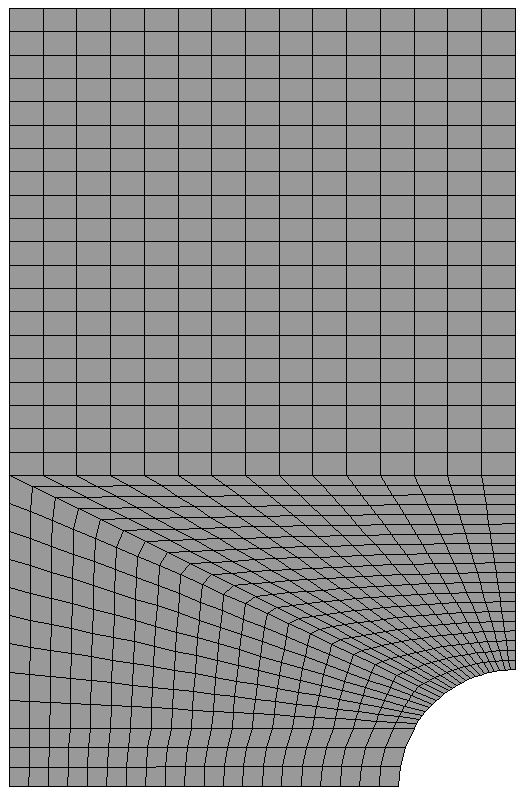
\includegraphics[width=1.16\textwidth]{25.0.5mm2.png}
         \caption{h=0.5 mm, n=840 elements}
         \label{fig:0.5mm}
     \end{subfigure}
     \hfill
     \begin{subfigure}{0.27\textwidth}
         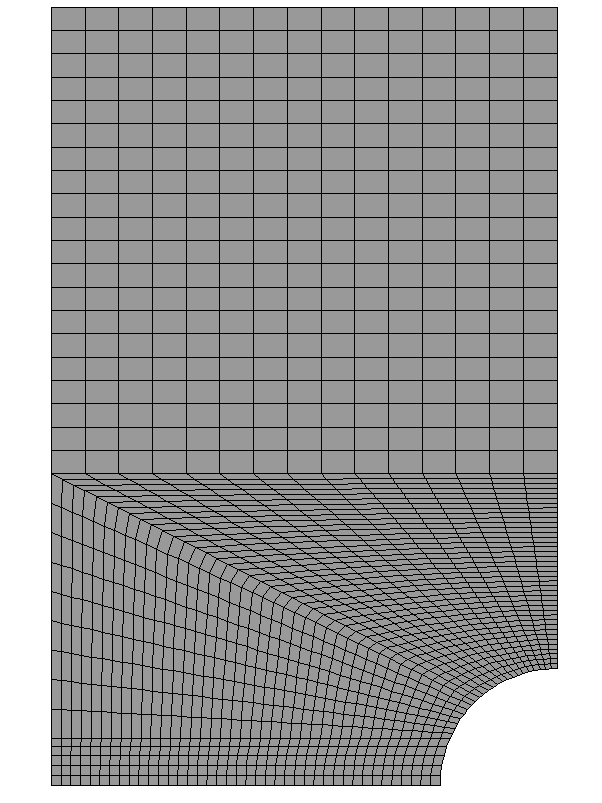
\includegraphics[width=1.14\textwidth]{25.0.25mm2.png}
         \caption{h=0.25 mm, n=1460 elements}
         \label{fig:0.25mm}
     \end{subfigure}
    \caption{Considered meshes (h is the length of the element along fracture zone and n the total number of elements) }
    \label{fig:Considered meshes}
\end{figure}
\FloatBarrier
\begin{figure}[htbp!]
       \begin{subfigure}{0.45\textwidth}
         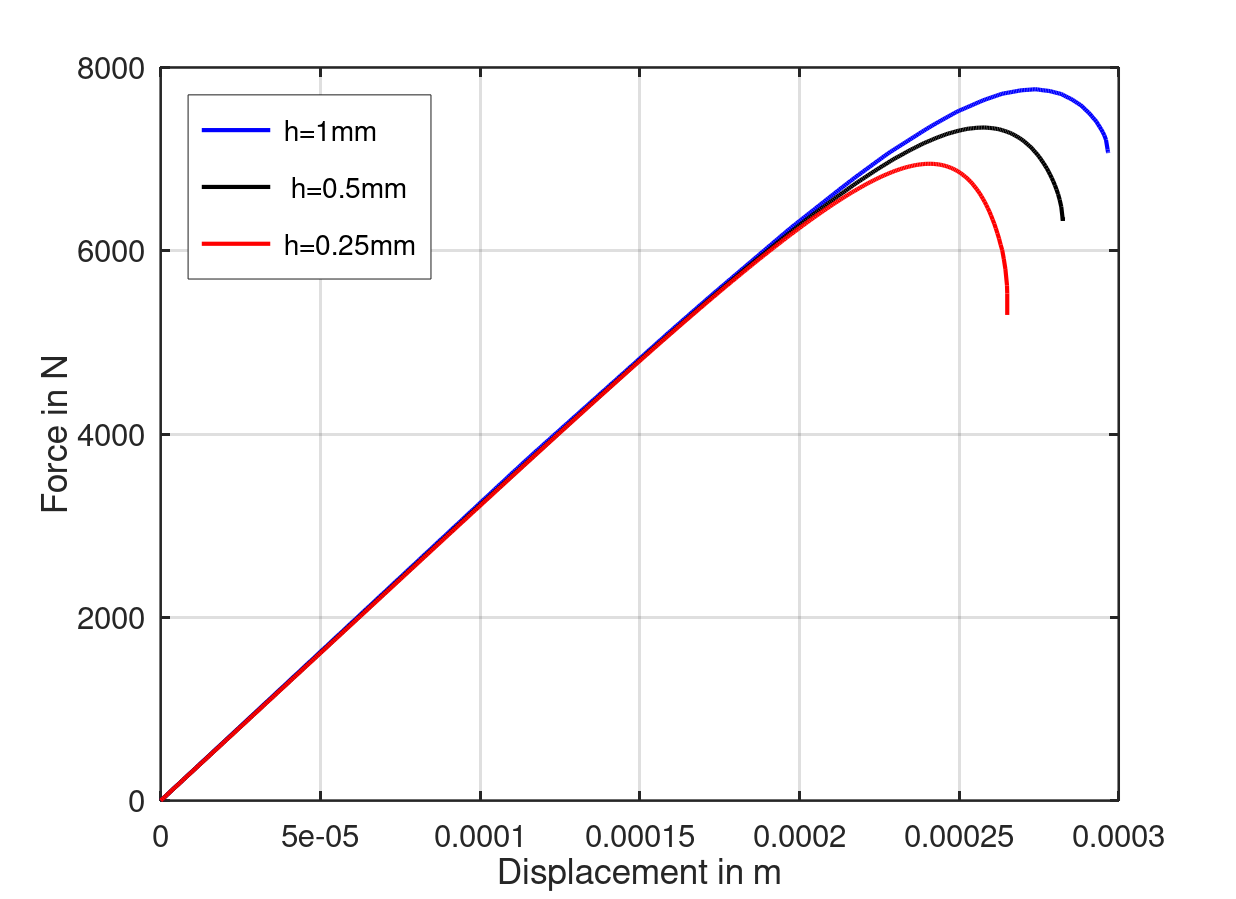
\includegraphics[width=8.5cm,height=7cm]{25.FvsD.png}
         \caption{model with regularization}
         \label{fig:with regularization}
     \end{subfigure}
     \hspace{1.5cm}
     \begin{subfigure}{0.45\textwidth}
         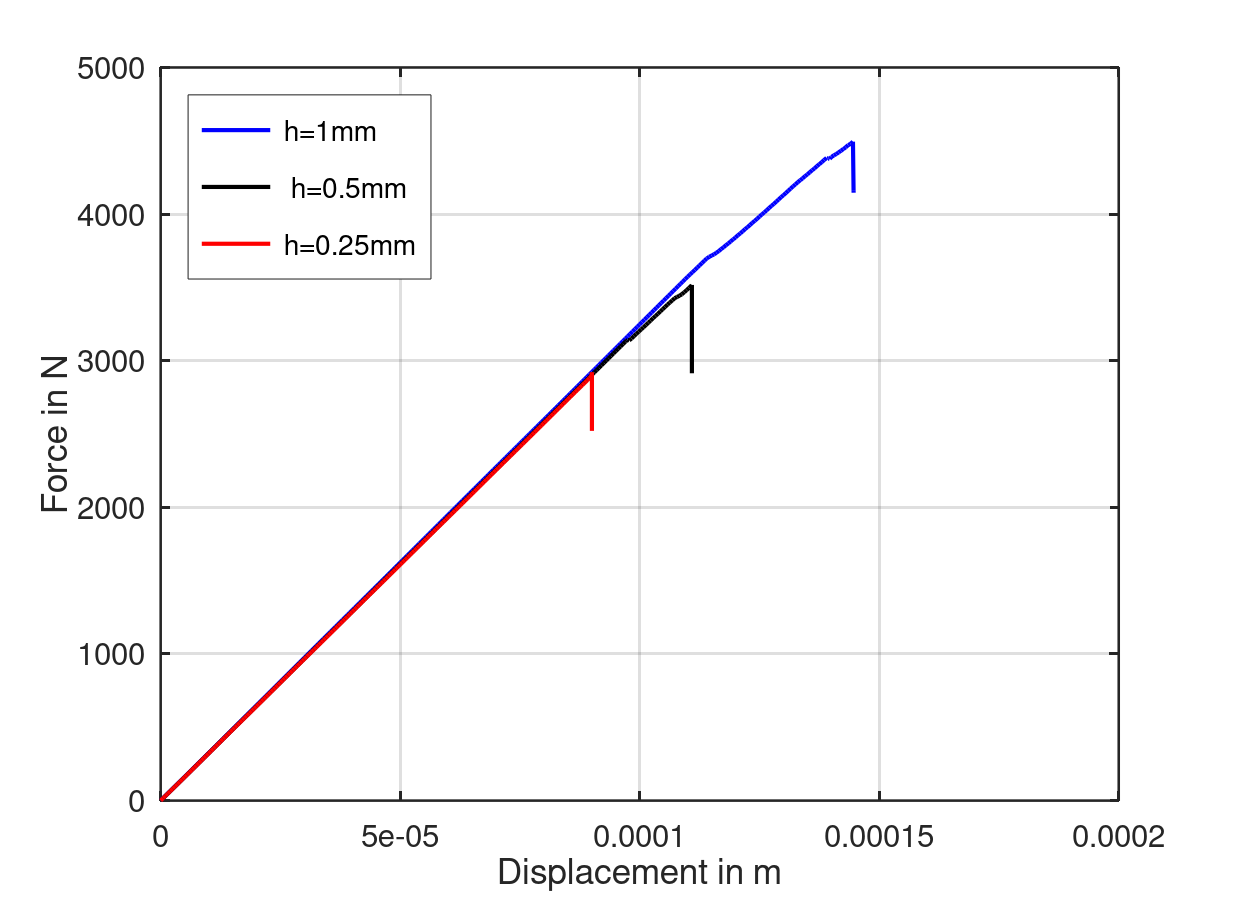
\includegraphics[width=8.5cm,height=7cm]{25.FvsD2.png}
         \caption{model without regularization}
         \label{fig:without regularization}
     \end{subfigure}
    \caption{Convergence study: Global force-displacement response for model with regularization (Figure a on the left) and without regularization (Figure b the right) }
    \label{fig:Convergence study}
\end{figure}
\FloatBarrier
 
\indent\indent\indent The damage distributions at the end of the process have been plotted for the three different meshes in the Figure (\ref{fig:Convergence study for model with and without regularization}). For numerical reasons the maximum damage is limited to a threshold value of $d_{max}$ = 0.999. The improvement in the global response by using regularization schemes has been illustrated by the damage distributions at the end of the loading process. A relatively large portion of the fracture zone takes part in the damage process instead of very few elements (one or two elements) in the case of no regularization. Damage initiates at the tip of the blunt notch and propagates perpendicular to the loading direction. The width of the damage zone is approximately the same in the three discretizations in the case of regularized models, but the number of elements that reach a critical damage value (red) increases with the increase in the number of elements along the fracture zone.

\begin{figure}[htbp!]
     \begin{subfigure}{0.4\textwidth}
         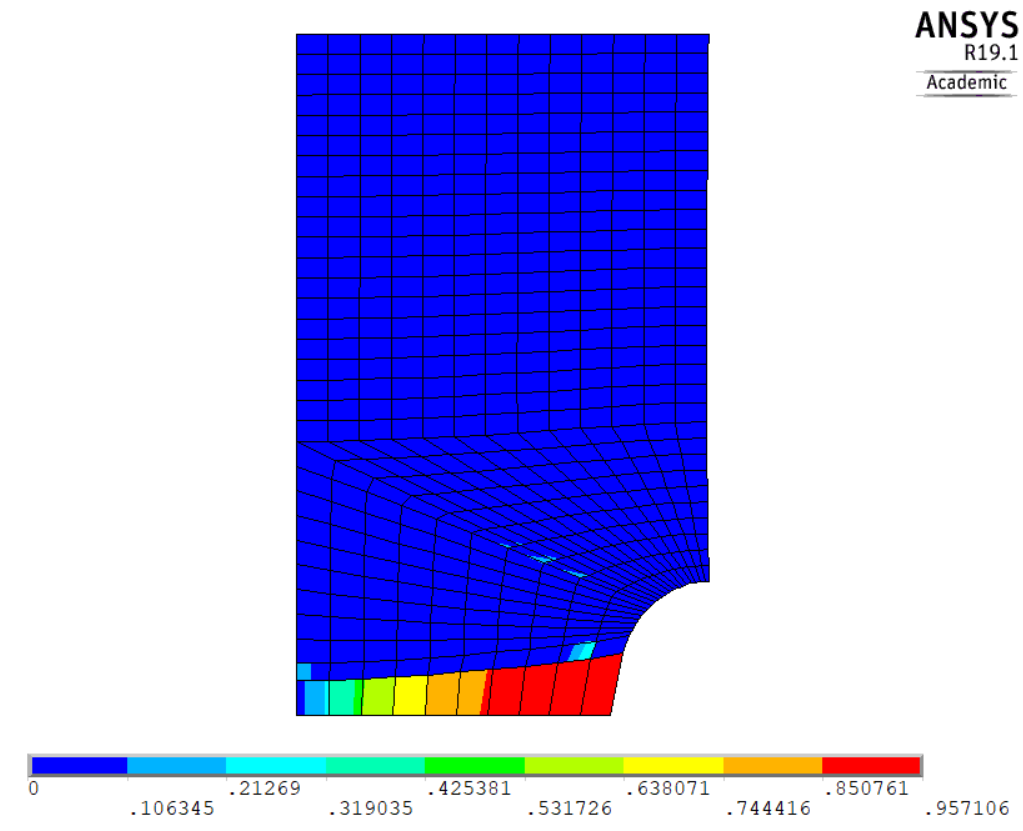
\includegraphics[width=8cm,height=7.2cm,keepaspectratio]{25.d1-1-r.png}
         \caption{h = 1 mm}
         \label{fig:d1-1-r}
     \end{subfigure}
    \hspace{1.8cm}
     \captionsetup[subfigure]{justification=centering}
     \begin{subfigure}{0.4\textwidth}
         \includegraphics[width=8cm,height=7.2cm,keepaspectratio]{25.d1-1-nr.png}
         \caption{h = 1 mm}
         \label{fig:d1-1-nr}
     \end{subfigure}
\end{figure}
\FloatBarrier
\begin{figure}[htbp!]\ContinuedFloat 
     \begin{subfigure}{0.4\textwidth}
         \includegraphics[width=8cm,height=7.2cm,keepaspectratio]{25.d1-0.5-r.png}
         \caption{h = 0.5 mm}
         \label{fig:d1-0.5-r}
     \end{subfigure}   
     \hspace{1.8cm}
     \begin{subfigure}{0.4\textwidth}
         \includegraphics[width=8cm,height=7.2cm,keepaspectratio]{25.d1-0.5-nr.png}
         \caption{h = 0.5 mm}
         \label{fig:d1-0.5-nr}
     \end{subfigure}
\end{figure}
\FloatBarrier
\begin{figure}[htbp!]\ContinuedFloat
     \begin{subfigure}{0.4\textwidth}
         \includegraphics[width=8cm,height=7.2cm,keepaspectratio]{25.d1-0.25-r.png}
         \caption{h = 0.25 mm}
         \label{fig:d1-0.25-r}
     \end{subfigure}
     \hspace{1.8cm}
     \begin{subfigure}{0.4\textwidth}
         \includegraphics[width=8cm,height=7.2cm,keepaspectratio]{25.d1-0.25-nr.png}
         \caption{h = 0.25 mm}
         \label{fig:d1-0.25-nr}
     \end{subfigure}     
        \caption{Convergence study for model with(Figure a,c,e) and without(b,d,f) regularization: Damage contour plots $d_{1}$ at the end of the loading}
        \label{fig:Convergence study for model with and without regularization}     
\end{figure}
\FloatBarrier
Now the transverse direction is kept parallel to the loading direction, and the behaviour of the damage model, i.e., initiation and propagation of damage $d_{2}$, is analysed by applying a tensile load in the transverse direction. The damage ($d_{2}$) at the end of the loading process is shown in the Figure (\ref{fig:Damage contour plots d2})
\\
\begin{figure}[htbp!]
 \centering
     \captionsetup[subfigure]{justification=centering}
     \begin{subfigure}{0.4\textwidth}
      \centering
         \includegraphics[width=8cm,height=7.2cm,keepaspectratio]{25.d2-1.png}
         \caption{h=1mm}
         \label{fig:d2-1}
     \end{subfigure}
     \hspace{1.8cm}
     \begin{subfigure}{0.4\textwidth}
      \centering
         \includegraphics[width=8cm,height=7.2cm,keepaspectratio]{25.d2-0.5.png}
         \caption{h=0.5mm}
         \label{fig:d2-0.5}
     \end{subfigure}
\end{figure}
\begin{figure}[htbp!]\ContinuedFloat
     \centering
     \begin{subfigure}{0.5\textwidth}
        \centering
        \includegraphics[width=8cm,height=7.2cm,keepaspectratio]{25.d2-0.25.png}
         \caption{h=0.25mm}
         \label{fig:d2-0.25}
     \end{subfigure}
    \caption{Damage contour plots $d_{2}$ at the end of the loading (Loading in transverse direction) }
    \label{fig:Damage contour plots d2}
\end{figure}
\FloatBarrier
The damage pattern looks similar to the distribution of damage ($d_{1}$) when loaded in the longitudinal direction. The force-displacement response of both longitudinal and transverse loading for a single mesh type (h = 0.5mm) is compared in the Figure (\ref{fig:Strength}). As expected, the maximum load capacity is high in the longitudinal direction compared to the transverse direction.

\begin{figure}[htbp!]
\begin{center}
\includegraphics[width=0.7\textwidth]{{25.Strength.png}}
 \caption{Comparison of force-displacement response in longitudinal and transverse direction for h = 0.5mm discretization}
 \label{fig:Strength}
 \end{center}
\end{figure}
\FloatBarrier 
 
\subsection{Compact Tension (CT) Specimen}\label{CT specimen}
\indent\indent\indent   This second example demonstrates the model's ability to compute multiple damage variables simultaneously, i.e., show the anisotropic damage development when a load is applied. In the plane stress (2D) setting, two damage variables ($d_{1}$ and $d_{2}$), one in each principal direction, are employed to represent the anisotropic damage development. The Compact Tension test is a standard test for plane fracture of materials and the measurement of fatigue crack growths. Because of the symmetry, only one half of the specimen is modelled, and the geometry and appropriate boundary conditions \citep{peerlings1999enhanced} are given in Figure (\ref{fig:CT Specimen}). The mesh consists of plane stress (PLANE 182) elements with bilinear interpolations for displacements, and 2*2 Gauss integration has been utilized. Just like the notched tensile specimen, three different finite element meshes have been used in the fracture zone with the elements of size h = 1 mm, 0.5 mm and 0.25 mm and a total of 509, 1409, 4811 elements, respectively for the convergence studies (Figure \ref{fig:Considered meshes 2}).  A node is created at the centre of the pinhole, and the innermost nodes of the pinhole contour are connected to this node by rigid coupling option in ANSYS. A displacement controlled load ($U_{x}$) is applied at the central node, and the global force-displacement response can be obtained from this central node.  At first, the longitudinal direction is kept parallel to the loading direction, and the behaviour of the model is analyzed.

\begin{figure}[htbp!]
\begin{center}
\includegraphics[width=0.8\textwidth]{{26.Geometry.jpg}}
 \caption{Specimen geometry and boundary conditions. Dimensions are given in mm. Displacement controlled loading $U_{x}$ is applied}
 \label{fig:CT Specimen}
 \end{center}
\end{figure}
\FloatBarrier  
\indent\indent\indent  The global force-displacement response has been plotted for the three different meshes in Figure (\ref{fig:CT Specimen FvsD}). As expected, the maximum load capacity decreases i.e., reduction in energy dissipation, with the decrease in mesh size (i.e., increase in the number of elements) because of the mesh dependence of the fracture energy-based damage evolution laws. The distributions of the damage variables $d_{1}$ and $d_{2}$ at the end of the loading process for the three different meshes have been plotted in Figure (\ref{fig: Damage contour plots d1 and d2}). The damage $d_{1}$ is caused by tension in the longitudinal direction and $d_{2}$ by tension in the transverse direction. The width of the damage zone for $d_{1}$ is approximately the same in all three discretizations. When the damage $d_{1}$ reaches the maximum threshold value in almost all the distorted elements, the simulations terminates; therefore, the maximum value and distribution of the damage variable $d_{2}$ depends on the size of the elements. From Figures (\ref{fig:d2-1}), (\ref{fig:d2-0.5}) and (\ref{fig:d2-0.25}) it is clearly evident that the maximum value and the width of the damage zone for $d_{2}$ increases with decrease in mesh size.
\begin{figure}[htbp!]
\hspace*{2cm}
  \captionsetup[subfigure]{justification=centering}
\begin{subfigure}{0.4\textwidth}
\begin{center}
\includegraphics[width=10cm,height=4.3cm]{26.h=1mm.png}
 \caption{h=1 mm}
 \label{fig:1mm}
  \end{center}
 \end{subfigure}
\end{figure}

\begin{figure}[htbp!]\ContinuedFloat
\hspace*{2cm}
\begin{subfigure}{0.4\textwidth}
\begin{center}
\includegraphics[width=10cm,height=4.3cm]{26.h=0.5mm.png}
 \caption{h=0.5 mm}
 \label{fig:0.5mm}
  \end{center}
 \end{subfigure}
\end{figure}
\FloatBarrier

\begin{figure}[htbp!]\ContinuedFloat
\hspace*{2cm}
\begin{subfigure}{0.4\textwidth}
\begin{center}
\includegraphics[width=10cm,height=4.3cm]{26.h=0.25mm.png}
 \caption{h=0.25 mm}
 \label{fig:0.25mm}
  \end{center}
 \end{subfigure}
     \caption{Considered meshes (h is the length of the element along fracture zone and n the total number of elements) }
    \label{fig:Considered meshes 2}
\end{figure}
\FloatBarrier


\begin{figure}[htbp!]
\begin{center}
\includegraphics[width=0.75\textwidth]{{26.FvsD.png}}
 \caption{Convergence study: Global force-displacement response for three different meshes}
 \label{fig:CT Specimen FvsD}
 \end{center}
\end{figure}
\FloatBarrier

\begin{figure}[htbp!]
       \captionsetup[subfigure]{justification=centering}
     \begin{subfigure}{0.4\textwidth}
          \includegraphics[width=8.25cm,height=8cm,keepaspectratio]{26.d1-1.png}
         \caption{d1, h = 1mm}
         \label{fig:d1-1}
     \end{subfigure}
    \hspace{2cm}
     \captionsetup[subfigure]{justification=centering}
     \begin{subfigure}{0.4\textwidth}
         \includegraphics[width=8.3cm,height=8cm,keepaspectratio]{26.d2-1.png}
         \caption{d2, h = 1mm}
         \label{fig:d2-1}
     \end{subfigure}
\end{figure}
\FloatBarrier
\begin{figure}[htbp!]\ContinuedFloat 
     \begin{subfigure}{0.4\textwidth}
         \includegraphics[width=8.2cm,height=8cm,keepaspectratio]{26.d1-0.5.png}
         \caption{d1, h = 0.5mm}
         \label{fig:d1-0.5}
     \end{subfigure}   
     \hspace{2cm}
     \begin{subfigure}{0.4\textwidth}
         \includegraphics[width=8.2cm,height=8cm,keepaspectratio]{26.d2-0.5.png}
         \caption{d2, h = 0.5mm}
         \label{fig:d2-0.5}
     \end{subfigure}
\end{figure}
\FloatBarrier
\begin{figure}[htbp!]\ContinuedFloat
     \begin{subfigure}{0.4\textwidth}
         \includegraphics[width=8.2cm,height=8cm,keepaspectratio]{26.d1-0.25.png}
         \caption{d1, h = 0.25mm}
         \label{fig:d1-0.25}
     \end{subfigure}
     \hspace{2cm}
     \begin{subfigure}{0.4\textwidth}
         \includegraphics[width=8.2cm,height=8cm,keepaspectratio]{26.d2-0.25.png}
         \caption{d2, h = 0.25mm}
         \label{fig:d2-0.25}
     \end{subfigure}     
        \caption{Damage distributions at the end of loading in longitudinal direction: Damage contour plots $d_{1}$ and $d_{2}$ }
        \label{fig: Damage contour plots d1 and d2}     
\end{figure}
\FloatBarrier 
\indent\indent\indent Now the transverse direction is kept parallel to the loading direction, and the anisotropic development of damage $d_{1}$ and $d_{2}$ is analysed. In this case, damage $d_{2}$ is the primary damage variable and damage $d_{1}$ is dependent on the mesh size.  The damage distributions ($d_{1}$ and $d_{2}$) for loading in transverse direction and force-displacement comparison of  longitudinal and transverse loading for h = 1mm discretization are shown in figure (\ref{fig:Damage contour plots d1 and d2 transverse direction}) and (\ref{fig:Strength2}) respectively.\\\\

\begin{figure}[htbp!]
      \begin{subfigure}{0.4\textwidth}
         \includegraphics[width=8.3cm,height=8cm,keepaspectratio]{26.d1_tran_1.png}
         \caption{$d_{1}$}
         \label{fig:d1_tran_0.5}
     \end{subfigure}
     \hspace{2cm}
     \begin{subfigure}{0.4\textwidth}
         \includegraphics[width=8.3cm,height=8cm,keepaspectratio]{26.d2_tran_1.png}
         \caption{$d_{2}$}
         \label{fig:d2_tran_0.5}
     \end{subfigure}
        \caption{Damage distributions at the end of loading in transverse direction: Damage contour plots $d_{1}$ and $d_{2}$ (h = 1mm discretization) }
        \label{fig:Damage contour plots d1 and d2 transverse direction}  
\end{figure}
\FloatBarrier
\begin{figure}[htbp!]
\begin{center}
\includegraphics[width=0.7\textwidth]{{26.Strength.png}}
 \caption{Comparison of force-displacement response in longitudinal and transverse direction for h = 1 mm discretization}
 \label{fig:Strength2}
 \end{center}
\end{figure}
\FloatBarrier
\subsubsection{Effect of shear in damage development}
\indent\indent\indent To deeply understand the failure of composite materials, the effect of shear on damage initiation and propagation is studied. The effect of shear stress in each failure mechanism is introduced by the modified Hashin's failure criterion (Section (\ref{Modified Hashin's failure criterion})) where $\alpha$ is the shear contribution factor which ranges from 0 to 1. The effect of shear can be studied by varying this shear contribution factor $\alpha$. 
\begin{figure}[htbp!]
\begin{center}
\includegraphics[width=0.73\textwidth]{{26.FvsD_alphas.png}}
 \caption{Comparison of force-displacement response for different shear co-efficient ($\alpha$) (h= 1mm discretization)}
 \label{fig:FvsD_alphas}
 \end{center}
\end{figure}
\FloatBarrier


The maximum value of $\alpha$ is chosen to be 0.5 to avoid the damage development only due to shear because the shear strength is low compared to other strengths. The global force-displacement response obtained for different $\alpha$ by loading the CT-Specimen in the longitudinal direction is shown in Figure (\ref{fig:FvsD_alphas}). It is evident that by increasing  $\alpha$, the failure index increases, which reduces the maximum load capacity of the CT specimen. 
 

\indent\indent\indent From Figure (\ref{fig:Stress_Comp}), it is clear that the increase in shear contribution has little to no effect in the initiation and distribution of the damage $d_{1}$ because the shear stress component ($\sigma_{12}$) is very low compared to the stress component ($\sigma_{11}$) which is responsible for damage $d_{1}$. However, the shear stress ($\sigma_{12}$) affects the damage $d_{2}$ because its magnitude is significant compared to the stress component ($\sigma_{22}$) which was the only component responsible for damage $d_{2}$ in the case of the maximum stress criterion.

\begin{figure}[htbp!]
\begin{center}
\includegraphics[width=0.75\textwidth]{{26.Stress_Comp.png}}
 \caption{Evolution of stress components during longitudinal tensile loading (h= 1mm discretization)}
 \label{fig:Stress_Comp}
 \end{center}
\end{figure}
\FloatBarrier
\indent\indent\indent The contour plots of damage $d_{2}$ for increasing shear contribution are plotted in Figure (\ref{fig:Damage contour plots alpha d2}). Compared to no shear effect ($\alpha$ = 0), the model with the presence of shear effect has more realistic damage propagation of ($d_{2}$), and the width of the damage zone is significantly larger. For the model with shear effect, the width of the damage zone is almost similar in all the cases, but the maximum damage value and the number of elements reaching critical damage value increase with the increase in $\alpha$.
\begin{figure}[htbp!]
       \captionsetup[subfigure]{justification=centering}
     \begin{subfigure}{0.4\textwidth}
         \includegraphics[width=8.3cm,height=8cm,keepaspectratio]{26.d2-1.png}
         \centering
         \caption{$\alpha$ = 0}
         \label{fig:d2-a_0}
     \end{subfigure}
     \hspace{2cm}
     \captionsetup[subfigure]{justification=centering}
     \begin{subfigure}{0.4\textwidth}
         \includegraphics[width=8.3cm,height=8cm,keepaspectratio]{26.d2_a_0.1.png}
         \caption{$\alpha$ = 0.1}
         \label{fig:d2-a_0.1}
     \end{subfigure}
\end{figure}
\FloatBarrier
\begin{figure}[htbp!]\ContinuedFloat
       \captionsetup[subfigure]{justification=centering}
     \begin{subfigure}{0.4\textwidth}
         \includegraphics[width=8.3cm,height=8cm,keepaspectratio]{26.d2_a_0.2.png}
         \caption{$\alpha$ = 0.2}
         \label{fig:d2-a_0.2}
     \end{subfigure}
    \hspace{2cm}
     \captionsetup[subfigure]{justification=centering}
     \begin{subfigure}{0.4\textwidth}
         \includegraphics[width=8.3cm,height=8cm,keepaspectratio]{26.d2_a_0.3.png}
         \caption{$\alpha$ = 0.3}
         \label{fig:d2-a_0.3}
     \end{subfigure}
\end{figure}
\FloatBarrier
\begin{figure}[htbp!]\ContinuedFloat
       \captionsetup[subfigure]{justification=centering}
     \begin{subfigure}{0.4\textwidth}
         \includegraphics[width=8.3cm,height=8cm,keepaspectratio]{26.d2_a_0.5.png}
         \caption{$\alpha$ = 0.5}
         \label{fig:d2-a_0.5}
     \end{subfigure}
        \caption{Damage distributions at the end of longitudinal loading: Damage contour plots $d_{2}$ for different shear co-efficients ($\alpha$)}
        \label{fig:Damage contour plots alpha d2} 
\end{figure}
\FloatBarrier
\indent\indent\indent In the case of transverse loading, the damage  $d_{2}$ is unaffected because the magnitude of the shear stress ($\sigma_{12}$) is very low compared to the stress ($\sigma_{22}$). However, the damage $d_{1}$ is affected because the magnitude of the shear stress component ($\sigma_{12}$) is similar compared to ($\sigma_{11}$).\\\\

\begin{figure}[htbp!]
\begin{center}
\includegraphics[width=0.75\textwidth]{{26.Stress_Comp2.png}}
 \caption{Evolution of stress components during transverse tensile loading (h= 1mm discretization)}
 \label{fig:Stress_Comp2}
 \end{center}
\end{figure}
\FloatBarrier
\begin{figure}[htbp!]
       \captionsetup[subfigure]{justification=centering}
     \begin{subfigure}{0.4\textwidth}
         \includegraphics[width=8.3cm,height=8cm,keepaspectratio]{26.d1_a_0.png}
         \caption{$\alpha$ = 0}
         \label{fig:d1-a_0}
     \end{subfigure}
    \hspace{2cm}
     \captionsetup[subfigure]{justification=centering}
     \begin{subfigure}{0.4\textwidth}
         \includegraphics[width=8.3cm,height=8cm,keepaspectratio]{26.d1_a_0.5.png}
         \caption{$\alpha$ = 0.5}
         \label{fig:d1-a_0.5}
     \end{subfigure}
             \caption{Damage distributions at the end of transverse loading: Damage contour plots $d_{1}$ for different shear co-efficient ($\alpha$)}
        \label{fig: Damage contour plots alpha d1} 
\end{figure}
\FloatBarrier

\clearpage
\subsection{Plate with hole (3D)}
\indent\indent\indent   This third example demonstrates the model's ability to show the anisotropic damage development for three dimensional (3D) problems. In 3D, three damage variables ($d_{1}$, $d_{2}$ and $d_{3}$) are employed to represent the anisotropic damage development, i.e., one damage variable for each principal material direction. Because of symmetry, only one-eighth of the specimen has been modelled. The geometry and the appropriate boundary conditions are given in Figure (\ref{fig:plate with hole}). Eight node solid elements (SOLID 185) with trilinear interpolations of the displacements and full integration has been used to perform the FE modelling. The thickness has been divided into four elements, and a fine mesh has been used in the region closer to the fracture zone shown in the Figure (\ref{fig:plate with hole mesh}).\\
 

\begin{figure}[htbp!]
\begin{center}
\includegraphics[width=1\textwidth]{{27.Geometry.jpg}}
 \caption{Specimen geometry and boundary conditions. Dimensions are given in mm. Displacement controlled loading $U_{x}$ is applied}
 \label{fig:plate with hole}
 \end{center}
\end{figure}
\FloatBarrier 


\indent\indent\indent The longitudinal direction is kept parallel to the loading direction, and the behaviour of the model is analysed by applying displacement controlled load ($U_{x}$) in the longitudinal direction (X-direction). The strength in transverse directions (2 and 3) are large enough for the damage variables $d_{2}$ and $d_{3}$ not to initiate when a longitudinal tensile load is applied. So to demonstrate the model's capability to show anisotropic damage development the transverse strength has been reduced  (For both tension and compression). The material properties considered for 3D damage model \citep{jiang2018evaluations} are given in the Table. (\ref{tab:Material parameters (3D Damage model)}). The maximum stress criterion (See Section(\ref{Maximum stress criteria})) has been used to predict the damage initiation in the three principal material directions. 



\begin{figure}[htbp!]
	\centering
       \captionsetup[subfigure]{justification=centering}
     \begin{subfigure}{0.5\textwidth}
     	\centering
         \includegraphics[width=9cm,height=10cm,keepaspectratio]{27.Mesh.png}
         \label{fig:plate with hole mesh 1}
     \end{subfigure}
    \hspace{1cm}
     \captionsetup[subfigure]{justification=centering}
     \begin{subfigure}{0.3\textwidth}
     \centering
         \includegraphics[width=8cm,height=8.5cm,keepaspectratio]{27.Mesh2.png}
         \label{fig:plate with hole mesh 2}
         \end{subfigure}
          \caption{Finite element discretization used for 3D damage study}
        \label{fig:plate with hole mesh} 
\end{figure}
\FloatBarrier 


\begin{table}[!htbp]
  \begin{center}
     \resizebox{15cm}{6.5cm}{
     \begin{tabular}{l l l} 
     \hline
     \\
      \textbf{Symbol} \;\;& \textbf{Material Parameter} \;& \textbf{Value}\\
      \\
      \hline
      \\
      \vspace*{0.1cm}
      $E_{11}$ & Modulus in longitudinal (1) direction &  55.8 GPa\\
      \vspace*{0.1cm}
      $E_{22}$ = $E_{33}$  & Modulus in transverse (2 and 3) directions   & 54.9 GPa \\
      \vspace*{0.1cm}
      $\nu_{12}$ =  $\nu_{13}$ & Poisson's ratio   & 0.043 \\
      \vspace*{0.1cm}
      $G_{12}$ =  $G_{23}$ = $G_{13}$   &  Shear modulus  & 4.2 GPa \\
      \vspace*{0.1cm}
      $X_{t}$ &  Tensile strength in longitudinal (1) direction & 910.1 MPa\\
      \vspace*{0.1cm}
      $X_{c}$ & Compressive strength in longitudinal (1) direction & -710.2 MPa\\
      \vspace*{0.1cm}
      $Y_{t}$ & Tensile strength in (2 and 3) directions  & 150 MPa\\
      \vspace*{0.1cm}
      $Y_{c}$ & Compressive strength in (2 and 3) directions &  -200 MPa\\
      \vspace*{0.1cm}
      $S_{12}$ & In-plane strength &  131 MPa\\
      \vspace*{0.1cm}
      $G_{f}^{lt}$ & Tensile fracture energy along longitudinal (1) direction  &  125 KJ/$m^{2}$\\
      \vspace*{0.1cm}
      $G_{f}^{lc}$ & Compressive fracture energy along longitudinal (1) direction  &  250 KJ/$m^{2}$\\
      \vspace*{0.1cm}
      $G_{f}^{tt}$ & Tensile fracture energy along (2 and 3) directions   &  95 KJ/$m^{2}$\\
      \vspace*{0.1cm}
      $G_{f}^{tc}$ & Compressive fracture energy along (2 and 3) directions  & 254 KJ/$m^{2}$\\
      \\
       \hline
    \end{tabular}
    }
    \\
    \caption{Material parameters (3D Damage model)}
    \label{tab:Material parameters (3D Damage model)}
  \end{center}
\end{table}
\FloatBarrier


\indent\indent\indent The global force-displacement response has been plotted for this longitudinal tensile loading in Figure (\ref{fig:plate with hole FvsD1}). The response is similar to the longitudinal loading in the notched tensile specimen, being characterized by a linear regime followed by a gradual drop of the load because of the softening. The softening is observed to initiate when the damage happens in critical number of elements in the fracture zone.
 
\begin{figure}[htbp!]
\begin{center}
\includegraphics[width=0.8\textwidth]{{27.FvsD1.png}}
 \caption{Global force-displacement response for the longitudinal tensile loading }
 \label{fig:plate with hole FvsD1}
 \end{center}
\end{figure}
\FloatBarrier 
\indent\indent\indent The damage distribution ($d_{1}$, $d_{2}$ and $d_{3}$) at the end of the tensile loading is shown in the Figure (\ref{fig:Contour plots of the damage d1,d2,d3}). In order to get a good visualization and understanding both element and nodal solution values of the damage are plotted. The initiation and evolution of damage $d_{1}$ is caused by the normal stress component $\sigma_{11}$ in the longitudinal direction.  The damage $d_{1}$ initiates at the tip of the blunt notch and then propagates perpendicular to the loading direction.\\

\indent\indent\indent From Figures (\ref{fig:d2-lt-e}) and (\ref{fig:d2-lt-n}) it is evident that the damage $d_{2}$ happens at two separate regions, i)\; perpendicular to the loading direction where damage $d_{1}$ already propagated ii)\; right at the blunt notch at the bottom edge of the plate. It has been observed that the damage $d_{2}$ in the region (i)\;happens because of tension in the transverse direction, and in the region (ii)\;the damage is caused by the compression in the transverse direction.  The propagation of damage $d_{3}$ is caused by the normal stress component $\sigma_{33}$ in the thickness direction. The damage $d_{2}$ and $d_{3}$ has much lesser influence on the strength of the specimen compared to the damage $d_{1}$ during longitudinal tensile loading.


\begin{figure}[htbp!]
     \captionsetup[subfigure]{justification=centering}
     \begin{subfigure}[htbp!]{0.4\textwidth}
     \begin{center}
         \includegraphics[width=8.2cm,height=9cm]{27.d1-lt-e.png}
         \caption{Damage $d_{1}$ - Element solution}
         \label{fig:d1-lt-e}
     \end{center}
     \end{subfigure}
     \hspace{1.9cm}
     \begin{subfigure}[htbp!]{0.4\textwidth}
         \includegraphics[width=8.2cm,height=9cm]{27.d1-lt-n.png}
         \caption{Damage $d_{1}$ - Nodal solution}
         \label{fig:d1-lt-n}
     \end{subfigure}
\end{figure}
\FloatBarrier
\vspace*{1.5cm}
\begin{figure}[htbp!]\ContinuedFloat     
     \begin{subfigure}[b]{0.4\textwidth}
        \includegraphics[width=8.2cm,height=9cm]{27.d2-lt-e.png}
         \caption{Damage $d_{2}$ - Element solution}
         \label{fig:d2-lt-e}
     \end{subfigure}
    \hspace{1.9cm}
      \begin{subfigure}[b]{0.4\textwidth}
         \includegraphics[width=8.2cm,height=9cm]{27.d2-lt-n.png}
         \caption{Damage $d_{2}$ - Nodal solution}
         \label{fig:d2-lt-n}
     \end{subfigure}
\end{figure}
\FloatBarrier
\begin{figure}[htbp!]\ContinuedFloat     
     \begin{subfigure}[b]{0.4\textwidth}
         \includegraphics[width=8.2cm,height=9cm]{27.d3-lt-e.png}
         \caption{Damage $d_{3}$ - Element solution}
         \label{fig:d3-lt-e}
     \end{subfigure}
     \hspace{1.9cm}
     \begin{subfigure}[b]{0.4\textwidth}
         \includegraphics[width=8.2cm,height=9cm]{27.d3-lt-n.png}
         \caption{Damage $d_{3}$ - Nodal solution}
         \label{fig:d3-lt-n}
     \end{subfigure}
        \caption{Contour plots of the damage distribution $d_{1}$, $d_{2}$ and $d_{3}$ at the end of longitudinal tensile loading }
        \label{fig:Contour plots of the damage d1,d2,d3}     
\end{figure}
\FloatBarrier

\indent\indent\indent These damage contour plots clearly indicate that the developed 3D model has the ability to show not only the damage development in three principal material directions but also both tension and compression damage happening simultaneously in a specimen when a load is applied.

\newpage
\fancyhead[RE,RO]{Summary and Conclusion} 
\chapter{Summary and Conclusion}
\indent\indent\indent The main aim of this thesis was to develop progressive damage models which can clearly describe the damage mechanism in composite materials when subject to various loading conditions. The models are developed using the framework of continuum damage mechanics (CDM). A second-order orthotropic damage tensor is employed to show the anisotropic damage development. A key issue in damage modelling is the convergence issue that arises due to the mesh dependant behaviour of the strain-softening models. The fracture energy regularization technique has been employed to reduce the mesh sensitivity, which ensures the objectivity of the model by adjusting dissipated energy to each finite element. At first, the damage models are implemented in octave and tested using constitutive driver routines for simple loading cases to verify the numerical implementation and understand the damage behaviour at integration point level, i.e., damage-evolution and strain-softening. During the integration point studies, it has been observed that the failure criteria, which uses strain to predict the damage initiation, cause convergence issues when damage evolves without the presence of stress in the given material direction, i.e. when transverse strength is very low, and a uniaxial tension is applied in the longitudinal direction. So the damage models implemented as user-defined material routines (USERMAT) in ANSYS employs stress-based failure criteria\\ 

\indent\indent\indent The user-defined material routines (USERMAT) are tested using a finite element of unit length in ANSYS to compare against the results from octave implementation. Once verified, representative structural examples (2D and 3D) are used to test the damage models in ANSYS to see how they predict the initiation and evolution of damage under various circumstances. Finite elements of varying sizes are used in the area prone to damage to analyze the mesh sensitivity of the damage models. It has been observed that the employed regularization scheme significantly improves the global response, but it does not fully alleviate the mesh dependency problems which arise due to strain-softening. Therefore a drop in maximum load capacity, i.e., reduction in energy dissipation, is observed in the global force-displacement response when the mesh is refined. Different failure criteria have been employed to see how the damage initiation and failure indices affect the model. It has been observed that the inclusion of the shear effect naturally reduces the maximum load capacity because of the increase in failure index for the same load. In some cases, the shear effect improves the damage behaviour when the magnitude of shear stress is significant compared to the normal stresses in the given material direction. Finally, the implemented damage models employing exponential damage evolution laws have the ability to represent the anisotropic damage development with the help of a second-order damage tensor and the strain-softening, which results from the stiffness degradation in 2D and 3D cases. This work provides a better understanding of the numerical implementation of the anisotropic damage models, which can predict the damage behaviour of complex composite materials.\\

The following changes and developments can be made in future to make this anisotropic damage model an excellent tool to analyze the complex damage phenomena in composite materials used in real-life applications
\begin{itemize}
\item By incorporating complex failure criteria like Linde's failure criteria, Hashin's quadratic failure criteria \citep{jiang2018evaluations} etc., the damage initiation and propagation can be predicted more accurately because of the inclusion of shear effects and quadratic terms.

\item From section (\ref{CT specimen}) (CT-Specimen), it is evident that when most of the distorted elements reach a critical value, the simulation terminates. This has been the case in most of the work done before. But in very few works \citep{jiang2018evaluations}, \citep{sokolinsky2011numerical} an option called element deletion (Available in the FEM software Abaqus) is employed to delete a particular failed element when the damage reaches a critical threshold value. This option can be included in the future to avoid the premature termination of analysis, and the whole crack propagation in the case of CT specimen can be simulated. 

\item Non-local gradient-enhanced damage formulations can be incorporated into the anisotropic damage models to eliminate the mesh dependency problems encountered in this work.  These non-local models use weighted volume averages of the state variables to create spatial interactions, which induces a smoothening effect on the deformation and damage.  Gradient enhanced formulations use higher-order deformation gradients of internal variables to create spatial discretization, eliminating the mesh dependency. Some of the works based on non-local damage models are \citep{peerlings1999enhanced}, \citep{fassin2019gradient}, \citep{geers1998experimental}, \citep{seupel2018efficient}


\end{itemize}





\newpage
\fancyhead[LE,LO]{Chapter 7} 
\fancyhead[RE,RO]{Bibliography} 
\bibliographystyle{plainnat}
\bibliography{reference}

\clearpage
\thispagestyle{empty}
\hfill
\clearpage
	\let\tmp\oddsidemargin
	\let\oddsidemargin\evensidemargin
	\let\evensidemargin\tmp
	\reversemarginpar
\pagenumbering{Roman}
\fancyhead[LE,LO]{Chapter 8} 
\fancyhead[RE,RO]{Appendix} 
\chapter*{Appendix}
\addcontentsline{toc}{chapter}{\textbf{Appendix}}

\renewcommand{\thesection}{\Alph{section}}
\setcounter{page}{\thesavepage}
\section{Stiffness matrix of the damaged material}\label{Stiffness matrix of the damaged material}
\subsection*{Plane stress (2D)}
The stiffness matrix of the damage material for plane-stress problems has the form \\

\begin{equation*}
\mathbb{C}(D) \; = \; \frac{1}{D}
 \begin{bmatrix}
  C_{11}(1 - d_{1}) & C_{12}(1 - d_{1})(1 - d_{2})  & 0 \\
  \\
  C_{21}(1 - d_{2})(1 - d_{1}) & C_{22}(1 - d_{2}) & 0 \\
 \\  
  0 & 0 &  D(1 - d_{3})G_{12} \\
  \\
 \end{bmatrix}
\end{equation*}

where $\mathlarger{D \; = \; 1 - (1 - d_{1})(1 - d_{2}) \nu_{12}\nu_{21}}$ and $\mathlarger{d_{3} \; = \; 1 - (1 - d_{1})(1 - d_{2}) }$



\subsection*{3D}
The stiffness matrix of the damage material for 3D problems has the form \\


$$
\mathbb{C}(D) \; = \; 
\begin{bmatrix}
\;C_{11}^{d} \; & \; C_{12}^{d}\; & \;C_{13}^{d} \; & \;0 \; & \;0 \; &\; 0 \;\\
  \\
 \; C_{21}^{d}\; & \;C_{22}^{d}\;  &\; C_{23}^{d}\; & \;0\; &\; 0\; & \; 0 \;\\
 \\  
 \; C_{31}^{d}\; & \; C_{32}^{d}\; &\; C_{33}^{d}\;  & \;0 \;& \;0 \;& \;0 \;\\
  \\
 \; 0 \; & \; 0 \; & \; 0 \; & \; C_{44}^{d} \;  & \; 0\; &\; 0\; \\
  \\
  \; 0 \; & \; 0 \; & \; 0\; &\; 0\; &\; C_{55}^{d}\; &\; 0\; \\
  \\
 \; 0\; & \;0 \;& \; 0\; &\; 0 \;& 0 \;& C_{66}^{d}\;
 \end{bmatrix}
$$
\\
\\
where \; $C_{ij}^{d}\; = \; (1 - d_{i})(1 - d_{j}), \; i,j \; = \; 1,2,3 $ \\
\\
 $C_{44}^{d}\; = \; (1 - d_{1})(1 - d_{2}), $ \\
 $C_{55}^{d}\; = \; (1 - d_{1})(1 - d_{3}),  $ \\
 $C_{66}^{d}\; = \; (1 - d_{2})(1 - d_{3}) $ \\
 
\definecolor{mygreen}{rgb}{0,0.6,0}
\definecolor{mygray}{rgb}{0.5,0.5,0.5}
\definecolor{mymauve}{rgb}{0.58,0,0.82}
\lstset{
basicstyle=\footnotesize,        % the size of the fonts that are used for the code
  breakatwhitespace=false,         % sets if automatic breaks should only happen at whitespace
  breaklines=false,                 % sets automatic line breaking
  captionpos=b,                    % sets the caption-position to bottom
  commentstyle=\color{black},    % comment style
  extendedchars=true,              % lets you use non-ASCII characters; for 8-bits encodings only, does not work with UTF-8
  keepspaces=true,                 % keeps spaces in text, useful for keeping indentation of code (possibly needs columns=flexible)
  keywordstyle=\color{black},       % keyword style
  language=[95]Fortran,                 % the language of the code
  numbers=left,                    % where to put the line-numbers; possible values are (none, left, right)
  numbersep=3pt,                   % how far the line-numbers are from the code
  numberstyle=\tiny\color{gray}, % the style that is used for the line-numbers
  rulecolor=\color{black},         % if not set, the frame-color may be changed on line-breaks within not-black text (e.g. comments (green here))
  showspaces=false,                % show spaces everywhere adding particular underscores; it overrides 'showstringspaces'
  showstringspaces=false,          % underline spaces within strings only
  showtabs=false,                  % show tabs within strings adding particular underscores
  stepnumber=1,                    % the step between two line-numbers. If it's 1, each line will be numbered
  stringstyle=\color{mymauve},     % string literal style
  tabsize=2,                       % sets default tabsize to 2 spaces
  title=\lstname                   % show the filename of files
}
 
\section{APDL Script}
\indent\indent\indent   The APDL script for simulating uniaxial tension in a unit cube is presented below
\begin{lstlisting}
/CLEAR

L = 1

STRETCH =0.2

/PREP7
!*  

ERESX,NO
ET,1,SOLID185
!*  
KEYOPT,1,2,0
KEYOPT,1,3,0
KEYOPT,1,6,0
KEYOPT,1,8,0
!*  

T1 = 1
TB,USER,1,1,9,9  
TBTEMP,T1
TBDATA,,55000e6,9500e6,9500e6,0.33,0.27,0.33,5500e6,3000e6,5500e6
TB,STATE,1,,7

MAT,1
TYPE,1

BLC4,0,0,L,L,L
ESIZE,,L
VMESH,1

NSEL,S,LOC,X,0
D,ALL,UX
NSEL,ALL

NSEL,S,LOC,Y,0
D,ALL,UY
NSEL,ALL

NSEL,S,LOC,Z,0
D,ALL,UZ
NSEL,ALL

/SOL
!*  
ANTYPE,0
NSUBST,100,10000,100
OUTRES,ERASE
OUTRES,ALL,ALL  
OUTRES,SVAR,ALL,,NSVAR
TIME,1

NSEL,S,LOC,X,L
D,ALL,UX,STRETCH
NSEL,ALL

/SOL
/STATUS,SOLU
SOLVE   


FINISH


\end{lstlisting}


\definecolor{mygreen}{rgb}{0,0.6,0}
\definecolor{mygray}{rgb}{0.5,0.5,0.5}
\definecolor{mymauve}{rgb}{0.58,0,0.82}
\lstset{
basicstyle=\footnotesize,        % the size of the fonts that are used for the code
  breakatwhitespace=false,         % sets if automatic breaks should only happen at whitespace
  breaklines=false,                 % sets automatic line breaking
  captionpos=b,                    % sets the caption-position to bottom
  commentstyle=\color{mygreen},    % comment style
  extendedchars=true,              % lets you use non-ASCII characters; for 8-bits encodings only, does not work with UTF-8
  keepspaces=true,                 % keeps spaces in text, useful for keeping indentation of code (possibly needs columns=flexible)
  keywordstyle=\color{blue},       % keyword style
  language=[95]Fortran,                 % the language of the code
  numbers=left,                    % where to put the line-numbers; possible values are (none, left, right)
  numbersep=3pt,                   % how far the line-numbers are from the code
  numberstyle=\tiny\color{gray}, % the style that is used for the line-numbers
  rulecolor=\color{black},         % if not set, the frame-color may be changed on line-breaks within not-black text (e.g. comments (green here))
  showspaces=false,                % show spaces everywhere adding particular underscores; it overrides 'showstringspaces'
  showstringspaces=false,          % underline spaces within strings only
  showtabs=false,                  % show tabs within strings adding particular underscores
  stepnumber=1,                    % the step between two line-numbers. If it's 1, each line will be numbered
  stringstyle=\color{mymauve},     % string literal style
  tabsize=2,                       % sets default tabsize to 2 spaces
  title=\lstname                   % show the filename of files
}

\newpage
\section{Source code for USERMAT}
\indent\indent\indent  The source code for the anisotropic damage model (in 3D) implemented as user material routine in ANSYS is given below

\begin{lstlisting}

  
        subroutine usermat(
     &                   matId, elemId,kDomIntPt, kLayer, kSectPt,
     &                   ldstep,isubst,keycut,
     &                   nDirect,nShear,ncomp,nStatev,nProp,
     &                   Time,dTime,Temp,dTemp,
     &                   stress,ustatev,dsdePl,sedEl,sedPl,epseq,
     &                   Strain,dStrain, epsPl, prop, coords, 
     &                   var0, defGrad_t, defGrad,
     &                   tsstif, epsZZ,
     &                   var1, var2, var3, var4, var5,
     &                   var6, var7, var8)
	
	
#include "impcom.inc"
#include "ansysdef.inc"
      integer :: matId, elemId, kDomIntPt, kLayer, kSectPt, ldstep,
     &           isubst,keycut, nDirect,nShear,ncomp,nStatev,nProp


      double precision :: Time,    dTime,   Temp,    dTemp,
     &                    sedEl,   sedPl,   epseq,   epsZZ
                  
      double precision :: stress  (ncomp  ), ustatev (nStatev), 
     &                 dsdePl  (ncomp,ncomp), Strain  (ncomp  ), 
     &                 dStrain (ncomp  ), epsPl   (ncomp  ),
     &                 prop    (nProp  ), coords  (3), 
     &                 defGrad (3,3),     defGrad_t(3,3),  
     &                 tsstif  (2) 
	
	
      EXTERNAL         usermat3d
      EXTERNAL         myuserfunc
      integer :: myvar
	
	
	
      double precision :: var0, var1, var2, var3, var4, var5,
     &                    var6, var7, var8

      integer :: iott,wrinqr
      external wrinqr
c
c*************************************************************************
c
      iott = wrinqr(WR_OUTPUT)
      write(iott,*) ' ************************************************'
      write(iott,*) ' * #DEBUG# UserMatLib.dll USERMAT               *'
      write(iott,*) ' ************************************************'
      myvar = 99
      call myuserfunc(myvar)
	
	

	if (ncomp >= 4) then
	
		
		call usermat3d (
     &                   matId, elemId,kDomIntPt, kLayer, kSectPt,
     &                   ldstep,isubst,keycut,
     &                   nDirect,nShear,ncomp,nStatev,nProp,
     &                   Time,dTime,Temp,dTemp,
     &                   stress,ustatev,dsdePl,sedEl,sedPl,epseq,
     &                   Strain,dStrain, epsPl, prop, coords,
     &                   var0, defGrad_t, defGrad,
     &                   tsstif, epsZZ,
     &                   var1, var2, var3, var4, var5,
     &                   var6, var7, var8)


      end if
      return
	end
	

      subroutine usermat3d(
     &                   matId, elemId,kDomIntPt, kLayer, kSectPt,
     &                   ldstep,isubst,keycut,
     &                   nDirect,nShear,ncomp,nStatev,nProp,
     &                   Time,dTime,Temp,dTemp,
     &                   stress,ustatev,dsdePl,sedEl,sedPl,epseq,
     &                   Strain,dStrain, epsPl, prop, coords, 
     &                   var0, defGrad_t, defGrad,
     &                   tsstif, epsZZ,
     &                   var1, var2, var3, var4, var5,
     &                   var6, var7, var8)
	
	
#include "impcom.inc"
#include "ansysdef.inc"
c
      integer :: matId, elemId, kDomIntPt, kLayer, kSectPt, ldstep,
     &           isubst,keycut, nDirect,nShear,ncomp,nStatev,nProp


      double precision :: Time,    dTime,   Temp,    dTemp,
     &                    sedEl,   sedPl,   epseq,   epsZZ
                  
      double precision :: stress  (ncomp  ), ustatev (nStatev), 
     &                 dsdePl  (ncomp,ncomp), Strain  (ncomp  ), 
     &                 dStrain (ncomp  ), epsPl   (ncomp  ),
     &                 prop    (nProp  ), coords  (3), 
     &                 defGrad (3,3),     defGrad_t(3,3),  
     &                 tsstif  (2)
	

	
	
********* USER DEFINED VARIABLES (FOR CALCULATION PURPOSE) **********	
	
      integer :: mcomp, twenty
      double precision :: HALF, ONE, TWO, ZERO,
     &                    THREE
      
      PARAMETER       (ZERO       = 0.d0,
     &                 HALF       = 0.5d0,
     &                 ONE        = 1.d0,
     &                 TWO        = 2.d0,
     &                 THREE      = 3.d0,
     &                 mcomp      = 6
     &                        )
	
      EXTERNAL          vzero, vmove
   
      double precision  dsdeEl(mcomp,mcomp), sigma(mcomp),
     &                  sigi (mcomp), C_T(mcomp,mcomp),
     &                  dsdeEl_d(mcomp,mcomp), T_strain(mcomp),
     &                  id(3,3), C_T_1(mcomp,mcomp),M_inv(mcomp,mcomp),
     &                  C_T_1_a(mcomp), C_T_0(mcomp,mcomp),
     &                  C_T_1_b(mcomp), C_T_2(mcomp,mcomp), 
     &                  C_T_2_a(mcomp),
     &                  C_T_2_b(mcomp),C_T_3(mcomp,mcomp), 
     &                  C_T_3_a(mcomp),
     &                  C_T_3_b(mcomp),sigma_eff(mcomp)
                  

      
      integer             i,j,k,l,n,P,ielem,iiter,key
      double precision    young_x, young_y, young_z,  
     &                    pr_xy, pr_yz, pr_xz, L_c,k1,k2,k3,d1_max,
     &                    xK, yield,G_c_1_t,G_c_1_c,G_c_2_t,G_c_2_c,
     &                    eps_11_f_t,eps_11_f_c,eps_22_f_t,d2_max,
     &                    eps_22_f_c,eps_33_f_t,eps_33_f_c,d3_max,
     &                    eps_12_f,eps_13_f,eps_23_f,sig_11_f_t,
     &                    sig_22_f_t,sig_33_f_t,d1,d2,d3,d1_new,d2_new
      
      double precision    d3_new,F_f,F_m,F_z,term1,term2,g_xy, g_yz, 
     &                    g_xz,delta,pr_yx, pr_zy, pr_zx,xy_yx, yz_zy,
     &                    zx_xz,xyz, E_xyz, sig_11_f_c, sig_22_f_c,
     &                    sig_33_f_c,sig_12_f,sig_23_f,sig_13_f,F_f_new,
     &                    F_m_new,F_z_new,V,term3,G_c_3_t,G_c_3_c

      
      
      double precision    var0, var1, var2, var3, var4, var5,
     &                    var6, var7, var8
	

    V    = ustatev(1)
    d1   = ustatev(2)
    d2   = ustatev(3)
    d3   = ustatev(4)
    F_f  = ustatev(5)
    F_m  = ustatev(6)
    F_z  = ustatev(7) 
      
c *** Receive material properties
	young_x  = prop(1)
	young_y  = prop(2)
	young_z  = prop(3)
	pr_xy    = prop(4)
	pr_yz    = prop(5)
	pr_xz    = prop(6)
	g_xy     = prop(7)
	g_yz     = prop(8)
	g_xz     = prop(9)
      
      
    sig_11_f_t = 910.1e6
    sig_11_f_c = -710.2e6
    sig_22_f_t =  150e6 
    sig_22_f_c = -200e6
    sig_33_f_t = 150e6
    sig_33_f_c = -200e6
    sig_12_f   = 131e6
    sig_13_f   = 131e6
    sig_23_f   = 131e6
    G_c_1_t    = 12.5e4
    G_c_1_c    = 25e4
    G_c_2_t    = 9.5e4
    G_c_2_c    = 25.4e4
    G_c_3_t    = 9.5e4
    G_c_3_c    = 25.4e4
    L_c        = V**(1.0/3.0)
    
   
      
	pr_yx = (young_y * pr_xy) / young_x
	pr_zy = (young_z * pr_yz) / young_y
	pr_zx = (young_z * pr_xz) / young_x
	
	
	xy_yx = pr_xy*pr_yx
	yz_zy = pr_yz*pr_zy 
	zx_xz = pr_zx*pr_xz
	xyz   = TWO*pr_xy*pr_yz*pr_zx
	E_xyz = young_x*young_y*young_z
	
	delta = (ONE - (xy_yx) - (yz_zy) - (zx_xz) - (xyz)) / E_xyz

    tsstif(1) = g_xz
    tsstif(2) = g_yz      

	


     
********* ELASTIC STIFFNESS MATRIX *********
	
	dsdeEl(1,1) = (ONE -yz_zy) / (young_y*young_z*delta)
	dsdeEl(1,2) = (pr_yx + pr_zx*pr_yz) / (young_y*young_z*delta)
	dsdeEl(1,3) = (pr_zx + pr_yx*pr_zy)/(young_y*young_z*delta)
    dsdeEl(1,4) = 0
	dsdeEl(1,5) = 0
	dsdeEl(1,6) = 0
	dsdeEl(2,1) = (pr_yx + pr_zx*pr_yz) /(young_y*young_z*delta)
    dsdeEl(2,2) = (ONE -zx_xz)/(young_x*young_z*delta)
	dsdeEl(2,3) = (pr_zy + pr_zx*pr_xy) /(young_x*young_z*delta) 
    dsdeEl(2,4) = 0
	dsdeEl(2,5) = 0
	dsdeEl(2,6) = 0
	dsdeEl(3,1) = (pr_zx + pr_yx*pr_zy) /(young_y*young_z*delta) 
    dsdeEl(3,2) = (pr_zy + pr_zx*pr_xy) / (young_x*young_z*delta)
    dsdeEl(3,3) = (ONE -xy_yx)/(young_x*young_y*delta)
	dsdeEl(3,4) = 0
	dsdeEl(3,5) = 0
	dsdeEl(3,6) = 0
	dsdeEl(4,1) = 0
	dsdeEl(4,2) = 0 
	dsdeEl(4,3) = 0
	dsdeEl(4,4) = g_xy
	dsdeEl(4,5) = 0
	dsdeEl(4,6) = 0
	dsdeEl(5,1) = 0
	dsdeEl(5,2) = 0 
	dsdeEl(5,3) = 0
	dsdeEl(5,4) = 0
	dsdeEl(5,5) = g_yz
	dsdeEl(5,6) = 0
	dsdeEl(6,1) = 0
	dsdeEl(6,2) = 0 
	dsdeEl(6,3) = 0
	dsdeEl(6,4) = 0
	dsdeEl(6,5) = 0
	dsdeEl(6,6) = g_xz

  
      
    eps_11_f_t = sig_11_f_t / ((ONE -yz_zy) / (young_y*young_z*delta))
    eps_11_f_c = sig_11_f_c / ((ONE -yz_zy) / (young_y*young_z*delta))
    eps_22_f_t = sig_22_f_t / ((ONE -zx_xz) / (young_x*young_z*delta))
    eps_22_f_c = sig_22_f_c / ((ONE -zx_xz) / (young_x*young_z*delta))
    eps_33_f_t = sig_33_f_t / ((ONE -xy_yx) / (young_x*young_y*delta))
    eps_33_f_c = sig_33_f_c / ((ONE -xy_yx) / (young_x*young_y*delta))
    eps_12_f   = sig_12_f / g_xy
    eps_13_f   = sig_13_f / g_xz 
    eps_23_f   = sig_23_f / g_yz

c *** Calculate current strain
      do i=1,ncomp
         T_strain(i) =  Strain(i) + dStrain(i) 
      end do

      
c**** Compute effective stress 
      call vzero(sigma_eff, 6)
      do i=1,ncomp
          do j=1,ncomp
              sigma_eff(i) = sigma_eff(i) + (dsdeEl(i,j)*T_strain(j))        
          end do
      end do        
      


      
c****Failure criteria
 
      if (sigma_eff(1) >= 0) then                    
          F_f_new = sigma_eff(1)/sig_11_f_t          
      else           
          F_f_new = sigma_eff(1)/sig_11_f_c  
      endif
            
      
      if (sigma_eff(2)>= 0)  then         
          F_m_new = sigma_eff(2)/sig_22_f_t     
      else          
          F_m_new = sigma_eff(2)/sig_22_f_c                
      endif
          
      
      if (sigma_eff(3) >= 0 )then      
          F_z_new = sigma_eff(3)/sig_33_f_t           
      else       
          F_z_new = sigma_eff(3)/sig_33_f_c                     
      endif
            
      
c******    To make sure failure indices are greater than or equal to previous step   *******   
      
      if (F_f_new >= F_f) then          
          F_f = F_f_new          
      else          
          F_f = F_f          
      endif
      
      if (F_m_new >= F_m) then          
          F_m = F_m_new          
      else          
          F_m = F_m          
      endif
          
      if (F_z_new >= F_z) then          
          F_z = F_z_new         
      else          
          F_z = F_z          
      endif
 
      
      
      call vzero(sigma,6)
      call vzero(C_T_1_a, 6) 
      call vzero(C_T_2_a, 6)
      call vzero(C_T_3_a, 6) 
      if ((F_f < 1) .AND. (F_m < 1) .AND. (F_z < 1)) then
 
c********    Update stress
        do i=1,ncomp
           sigma(i) = sigma_eff(i)       
        end do 
          

      
      else
          
c*********  Softening parameter  ***********
        if (sigma_eff(1) >= 0) then
          k1 =   (-sig_11_f_t*eps_11_f_t*L_c)/G_c_1_t
        else 
          k1 =   (-sig_11_f_c*eps_11_f_c*L_c)/G_c_1_c
        endif
        
        
        if (sigma_eff(2)  >= 0) then
          k2 =  (-sig_22_f_t*eps_22_f_t*L_c)/G_c_2_t
        else 
          k2 =  (-sig_22_f_c*eps_22_f_c*L_c)/G_c_2_c
        endif
      
        
        if (sigma_eff(3) >= 0) then
          k3 =  (-sig_33_f_t*eps_33_f_t*L_c)/G_c_3_t
        else 
          k3 =  (-sig_33_f_c*eps_33_f_c*L_c)/G_c_3_c
        endif
       
        d1_max = 0.999
        d2_max = 0.999
        d3_max = 0.999
        
c*********   Damage evolution equations    *********** 	  
        if (F_f >= 1) then
      
          d1_new = d1_max*(ONE  - (exp(k1*(F_f - ONE)))/F_f)
          
          if (d1_new > d1) then
              d1 = d1_new
          else
              d1 = d1
          endif          
     
        endif        

      
        if (F_m >= 1) then
      
          d2_new =  d2_max*(ONE  - (exp(k2*(F_m- ONE)))/F_m)
          
          if (d2_new > d2) then
              d2 = d2_new
          else
              d2 = d2
          endif      
      
        endif
      
      
        if (F_z >= 1) then
      
          d3_new = d3_max*(ONE  - (exp(k3*(F_z - ONE)))/F_z)
          
          if (d3_new > d3) then
              d3 = d3_new
          else
              d3 = d3
          endif      
          
        endif 
        

        
        
c*****      Inverse of the damage effect tensor  ********
        
        do i = 1,ncomp
            do j= 1,ncomp
                M_inv(i,j) = ZERO
            end do
        end do
        
        M_inv(1,1)  = (1 - d1)
        M_inv(2,2)  = (1 - d2)
        M_inv(3,3)  = (1 - d3)
        M_inv(4,4)  = sqrt((1 - d1)*(1 - d2))
        M_inv(5,5)  = sqrt((1 - d3)*(1 - d2))
        M_inv(6,6)  = sqrt((1 - d1)*(1 - d3))
        
c*******   Find nominal stress from effective stress ********
        do i=1,ncomp
           do j=1,ncomp
               sigma(i) = sigma(i) + (M_inv(i,j)*sigma_eff(j))        
           end do
        end do        


c********      Degraded stiffness   **********      
        dsdeEl_d(1,1)=(ONE-yz_zy)/(young_y*young_z*delta)*(ONE
     &                -d1)**2
        dsdeEl_d(1,2) = (pr_yx + pr_zx*pr_yz) / (young_y*young_z*delta)
     &              *(ONE - d1)*(ONE - d2)
        dsdeEl_d(1,3) = (pr_zx + pr_yx*pr_zy) / (young_y*young_z*delta)*
     &              (ONE - d1)*(ONE - d3)
        dsdeEl_d(1,4) = 0
        dsdeEl_d(1,5) = 0
        dsdeEl_d(1,6) = 0
        dsdeEl_d(2,1) = (pr_yx + pr_zx*pr_yz) / (young_y*young_z*delta)*
     &              (ONE - d1)*(ONE - d2)
        dsdeEl_d(2,2)=(ONE -zx_xz)/(young_x*young_z*delta)*(ONE - d2)**2
        dsdeEl_d(2,3) = (pr_zy + pr_zx*pr_xy)/(young_x*young_z*delta)*
     &              (ONE - d3)*(ONE - d2)
        dsdeEl_d(2,4) = 0
        dsdeEl_d(2,5) = 0
        dsdeEl_d(2,6) = 0
        dsdeEl_d(3,1) = (pr_zx + pr_yx*pr_zy) /(young_y*young_z*delta)*
     &              (ONE - d3)*(ONE - d1)
        dsdeEl_d(3,2) = (pr_zy + pr_zx*pr_xy) / (young_x*young_z*delta)*
     &              (ONE - d3)*(ONE- d2)
        dsdeEl_d(3,3) = (ONE -xy_yx)/(young_x*young_y*delta)*(ONE
     &                -d3)**2
        dsdeEl_d(3,4) = 0
        dsdeEl_d(3,5) = 0
        dsdeEl_d(3,6) = 0
        dsdeEl_d(4,1) = 0
        dsdeEl_d(4,2) = 0 
        dsdeEl_d(4,3) = 0
        dsdeEl_d(4,4) = g_xy*(ONE - d1)*(ONE - d2)
        dsdeEl_d(4,5) = 0
        dsdeEl_d(4,6) = 0
        dsdeEl_d(5,1) = 0
        dsdeEl_d(5,2) = 0 
        dsdeEl_d(5,3) = 0
        dsdeEl_d(5,4) = 0
        dsdeEl_d(5,5) = g_yz*(ONE - d2)*(ONE - d3)
        dsdeEl_d(5,6) = 0
        dsdeEl_d(6,1) = 0
        dsdeEl_d(6,2) = 0 
        dsdeEl_d(6,3) = 0
        dsdeEl_d(6,4) = 0
        dsdeEl_d(6,5) = 0
        dsdeEl_d(6,6) = g_xz*(ONE - d3)*(ONE - d1)
        
        if ((d1 == ZERO))then
          
          do i=1,mcomp
             do j=1,mcomp
                 C_T_1(i,j) = 0        
             end do
          end do  
          
        else
            
          C_T_1_a =(/-sigma_eff(1),ZERO,ZERO,(HALF*(d2- 1)*sigma_eff(4))
     &    /M_inv(4,4),ZERO,(HALF*(d3 - 1)*sigma_eff(6))/M_inv(6,6)/) 
 
          
c**********   Derivative of d1 with respect to strain (d_d1/d_epsilon)   ***********
 
c**       For Tension          
          if (sigma_eff(1)> 0)  then
              
            term1 = d1_max*(((ONE-k1*F_f)*exp(k1*(F_f - ONE)))/(F_f**2))
          
            C_T_1_b  = (/ (term1*dsdeEl(1,1))/sig_11_f_t,
     &      (term1*dsdeEl(1,2))/sig_11_f_t,(term1*dsdeEl(1,3))
     &      /sig_11_f_t,ZERO,ZERO,ZERO/)

            
c**       For Compression           
          else
              
            term1 = d1_max*(((ONE-k1*F_f)*exp(k1*(F_f - ONE)))/(F_f**2))
          
            C_T_1_b  = (/ (term1*dsdeEl(1,1))/sig_11_f_c,
     &      (term1*dsdeEl(1,2))/sig_11_f_c,(term1*dsdeEl(1,3))
     &      /sig_11_f_c,ZERO,ZERO,ZERO/)
            
          endif
      
          do i = 1,mcomp
              do j = 1,mcomp
                  C_T_1(i,j) = C_T_1_a(i)*C_T_1_b(j)
              end do
          end do
       
        endif
            
        

        if ((d2 == ZERO)) then
          
          do i=1,mcomp
             do j=1,mcomp
                 C_T_2(i,j) = 0        
             end do
          end do 
      
        else 
            
          C_T_2_a =(/ZERO,-sigma_eff(2),ZERO,(HALF*(d1- 1)*sigma_eff(4))
     &    /M_inv(4,4),(HALF*(d3 - 1)*sigma_eff(5))/M_inv(5,5),ZERO /) 
          
c******     Derivative of d2 with respect to strain (d_d2/d_epsilon)
      
c****      For Tension           
          if (sigma_eff(2)> 0)  then
              
            term2 = d2_max*(((ONE-k2*F_m)*exp(k2*(F_m - ONE)))/(F_m**2))
          
            C_T_2_b  = (/ (term2*dsdeEl(2,1))/sig_22_f_t, 
     &     (term2*dsdeEl(2,2))/sig_22_f_t,(term2*dsdeEl(2,3))
     &     /sig_22_f_t,ZERO,ZERO,ZERO/) 
     
c**       For Compression                       
          else                                         
              
            term2 = d2_max*(((ONE-k2*F_m)*exp(k2*(F_m - ONE)))/(F_m**2))
          
            C_T_2_b  = (/ (term2*dsdeEl(2,1))/sig_22_f_c, 
     &     (term2*dsdeEl(2,2))/sig_22_f_c,(term2*dsdeEl(2,3))
     &     /sig_22_f_c,ZERO,ZERO,ZERO/) 
            
          endif

              
          do i = 1,mcomp
              do j = 1,mcomp
                  C_T_2(i,j) = C_T_2_a(i)*C_T_2_b(j)
              end do
          end do              
              
        endif      
      
      
        if ((d3 == ZERO))then
      
              do i=1,ncomp
                 do j=1,ncomp
                     C_T_3(i,j) = 0        
                 end do
              end do 
          
        else 
            
          C_T_3_a = (/ZERO,ZERO,-sigma_eff(3), ZERO,
     &    (HALF*(d2 - 1)*sigma_eff(5))/M_inv(5,5),(HALF*(d1 - 1)
     &    *sigma_eff(6))/M_inv(6,6) /) 
          
c*****     Derivative of d3 with respect to strain (d_d3/d_epsilon)
          
c****     For Tension 
          if (sigma_eff(3) > 0) then
              
            term3 = d3_max*(((ONE-k3*F_z)*exp(k3*(F_z - ONE)))/(F_z**2))  
              
            C_T_3_b  = (/ (term3*dsdeEl(3,1))/sig_33_f_t,
     &    (term3*dsdeEl(3,2))/sig_33_f_t,(term3*dsdeEl(3,3))/sig_33_f_t,
     &    ZERO,ZERO,ZERO/)   
              
c****     For Compression              
          else 
              
            term3 = d3_max*(((ONE-k3*F_z)*exp(k3*(F_z - ONE)))/(F_z**2))  
              
            C_T_3_b  = (/ (term3*dsdeEl(3,1))/sig_33_f_c,
     &    (term3*dsdeEl(3,2))/sig_33_f_c,(term3*dsdeEl(3,3))/sig_33_f_c,
     &    ZERO,ZERO,ZERO/)  
            
          endif
          
          do i = 1,mcomp
              do j = 1,mcomp
                  C_T_3(i,j) = C_T_3_a(i)*C_T_3_b(j)
              end do
          end do 
          
        endif


        do i = 1,ncomp
            do j= 1,ncomp
                C_T(i,j) = ZERO
            end do
        end do
c*********   Tangent stiffness  
        do i=1,ncomp
           do j=1,ncomp
              C_T(i,j)   =  dsdeEl_d(i,j) +  C_T_1(i,j) + C_T_2(i,j) +
     &        C_T_3(i,j) 
           end do
        end do
      
            
      endif
      

      ustatev(2) = d1
      ustatev(3) = d2
      ustatev(4) = d3
      ustatev(5) = F_f
      ustatev(6) = F_m
      ustatev(7) = F_z

      call vzero(stress,6)
c *** Update stress i
      do i=1,ncomp
         stress(i) = sigma(i)
      end do
      
      
 

      

      
      if ((F_f < 1) .AND. (F_m < 1) .AND. (F_z < 1)) then
          
          do i=1,ncomp
              do j=1,ncomp
                  dsdePl(i,j) = dsdeEl(i,j)        
              end do
          end do 
      
      else
          
          do i=1,ncomp
              do j=1,ncomp
                  dsdePl(i,j) = C_T(i,j)        
              end do
          end do 
          
      endif  
      
      
      
      return
      end
	
\end{lstlisting}

              
              
              
              
              
              
              
              
              
              
              
              
              
              
              
              
              
              
              
              
              
              
              
              
              
              
              
              
              
              
              

      

      
      
      
      
      
      
      
      
      
      
      
      
      
      
      
      
      
      
      
      
      
      
      
      
      
      
      
      
      
      
      
      
      
      
      
      
      
      
      
      
      
      
      
      
      
      
      
      
      
      
      
      
      
      
      
      
      
      
      
      
      
      
      
      
      
      
      
      
      
      
      
      
      
      
      
      
      
      
      
      
      
      
      
      
      
      
      
      
      
      
      
      
      
      
      
      
      
      
      
      
      
      
      
      
      
      
      
      
      
      
      
      
      
      
      
      
      
      
      
      
      
      
      
      
      
      
      
      
      
      
      
      
      
      
      
      
      
      
      
      
      
      
      
      
      
      
      
      
      
      
      
      
      
      
      
      
      
      
      
      
      
      
      
      
      
      
      
      
      
      
      
      
      
      
      
      
      
      
      
      
      
      
      
      
      
      
      
      
      
      
      
      
      
      
      
      
      
      
      
      
      
      
      
      
      
      
      
      
      
      
      
      
      
      
      
      
      
      
      
      
      
      
      
      
      
      
      
      
      
      
      
      
      
      
      
      
      
      
      
      
      
      
      
      
      
      
      
      
      
      
      
      
      
      
      
      
      
      
      
      
      
      
      
      
      
      
      
      
      
      
      
      
      
      
      
      
      
      
      
      
      
      
      
      
      
      
      
      
      
      
      
      
      
      
      
      
      
      
      
      
      
      
      
      
      
      
      
      
      
      
      
      
      
      
      
      
      
      
      
      
      
      
      
      
      
      
      
      
      
      
      
      
      
      
      
      
      
      
      
      
      
      
      
      
      
      
      
      
      
      
      
      
      
      
      
      
      
      
      
      
      
      
      
      
      
      
      
      
      
      
      
      
      
      
      
      
      
      
      
      
      
      
      
      
      
      
      
      
      
      
      
      
      
      
      
      
      
      
      
      
      
      
      
      
      
      
      
      
      
      
      
      
      
      
      
      
      
      
      
      
      
      
      
      
      
      
      
      
      
      
      
      
      
      
      
      
      
      
      
      
      
      
      
      
      
      
      
      
      
      
      
      
      
      
      
      
      
      
      
      
      
      
      
      
      
      
      
      
      
      
      
      
      
      
      
      
      
      
      
      
      
      
      
      
      
      
      
      
      
      
      
      
      
      
      
      
      
      
      
      
      
      
      
      
      
      
      
      
      
      
      
      
      
      
      
      
      
      
      
      
      
      
      
      
      
      
      
      
      
      
      
      
      
      
      
      
      
      
      
      
      
      
      
      
      
      
      
      
      
      
      
      
      
      
      
      
      
      
      
      
      
      
      
      
      
      
      
      
      
      
      
      
      
      
      
      
      
      
      
      
      
      
      
      
      
      
      
      
      
      
      
      
      
      
      
      
      
      
      
      
      
      
      
      
      
      
      
      
      
      
      
      
      
      
      
      
      
      
      
      
      
      
      
      
      
      
      
      
      
      
      
      
      
      
      
      
      
      
      
      
      
      
      
      
      
      
      
      
      
      
      
      
      
      
      
      
      
      
      
      
      
      
      
      
      
      
      
      
      
      
      
      
      
      
      
      
      
      
      
      
      
      
      
      
      
      
      
      
      
      
      
      
      
      
      
      
      
      
      
      
      
      
      
      
      
      
      
      
      
      
      
      
      
      
      
      
      
      
      
      
      
      
      
      
      
      
      
      
      
      
      
      
      
      
      
      
      
      
      
      
      
      
      
      
      
      
      
      
      
      
      
      
      
      
      
      
      
      
      
      
      
      
      
      
      
      
      
      
      
      
      
      
      
      
      
      
      
      
      
      
      
      
      
      
      
      
      
      
      
      
      
      
      
      
      
      
      
      
      
      
      
      
      
      
      
      
      
      
      
      
      
      
      
      
      
      
      
      
      
      
      
      
      
      
      
      
      
      
      
      
      
      
      
      
      
      
      
      
      
      
      
      
      
      
      
      
      
      
      
      
      
      
      
      
      
      
      
      
      
      
      
      
      
      
      
      
      
      
      
      
      
      
      
      
      
      
      
      
      
      
      
      
      
      
      
      
      
      
      
      
      
      
      
      
      
      
      
      
      
      
      
      
      
      
      
      
      
      
      
      
      
      
      
      
      
      
      
      
      
      
      
      
      
      
      
      
      
      
      
      
      
      
      
      
      
      
      
      
      
      
      
      
      
      
      
      
      
      
      
      
      
      
      
      
      
      
      
      
      
      
      
      
      
      
      
      
      
      
      
      
      
      
      
      
      
      
      
      
      
      
      
      
      
      
      
      
      
      
      
      
      
      
      
      
      
      
      
      
      
      
      
      
      
      
      
      
      
      
      
      
      
      
      
      
      
      
      
      
      
      
      
      
      
      
      
      
      
      
      
      
      
      
      
      
      
      
      
      
      
      
      
      
      
      
      
      
      
      
      
      
      
      
      
      
      
      
      
      
      
      
      
      
      
      
      
      
      
      
      
      
      
      
      
      
      
      
      
      
      
      
      
      
      
      
      
      
      
      
      
      
      
      
      
      
      
      
      
      
      
      
      
      
      
      
      
      
      
      
      
      
      
      
      
      
      
      
      
      
      
      
      
      
      
      
      
      
      
      
      
      
      
      
      
      
      
      
      
      
      
      
      
      
      
      
      
      
      
      
      
      
      
      
      
      
      
      
      
      
      
      
      
      
      
      
      
      
      
      
      
      
      
      
      
      
      
      
      
      
      
      
      
      
      
      
      
      
      
      
      
      
      
      
      
      
      
      
      
      
      
      
      
      
      
      
      
      
      
      
      
      
      
      
      
      
      
      
      
      
      
      
      
      
      
      
      
      
      
      
      
      
      
      
      
      
      
      
      
      
      
      
      
      
      
      
      
      
      
      
      
      
      
      
      
      
      
      
      
      
      
      
      
      
      
      
      
      
      
      
      
      
      
      
      
      
      
      
      
      
      
      
      
      
      
      
      
      
      
      
      
      
      
      
      
      
      
      
      
      
      
      
      
      
      
      
      
      
      
      
      
      
      
      
      
      
      
      
      
      
      
      
      
      
      
      
      
      
      
      
      
      
      
      
      
      
      
      
      
      
      
      
      
      
      
      
      
      
      
      
      
      
      
      
      
      
      
      
      
      
      
      
      
      
      
      
      
      
      
      
      
      
      
      
      
      
      
      
      
      
      
      
      
      
      
      
      
      
      
      
      
      
      
      
      
      
      
      
      
      
      
      
      
      
      
      
      
      
      
      
      
      
      
      
      
      
      
      
      
      
      
      
      
      
      
      
      
      
      
      
      
      
      
      
      
      
      
      
      


\end{document}
